%%%%%%%%%%%%%%%%%%%%%%%%%%%%%%%%%%%%%%%%%%%%%%%%%%%%%%%%%%%%%%%%%%%%%%%%%%%%%%%
% Author:  Reinaldo Castro González
% 
% Este documento está basado en la tesis del M.Sc. Carlos Salazar
%
% Según la plantilla desarrollada por el Dr. Pablo Alvarado
%
% Escuela de Ingeniería Electrónica
% Instituto Tecnológico de Costa Rica
%
% Tesis de Licenciatura
% 
% Phone:   +506 2550 2106
% Fax:     +506 2591 6629
% email:   palvarado@ietec.org
%
% $Id: main.tex 1513 2010-08-15 01:25:24Z palvarado $
%
%%%%%%%%%%%%%%%%%%%%%%%%%%%%%%%%%%%%%%%%%%%%%%%%%%%%%%%%%%%%%%%%%%%%%%%%%%%%%%%

% \documentclass is book
\documentclass[12pt,twoside,letterpaper]{book}

\usepackage[utf8]{inputenc}
\usepackage{ifthen}                     % provide if-then-else operators
\usepackage{listings}
%\usepackage{verbatim}
\usepackage{paralist} %fancy list of figures
\usepackage{multirow}
\usepackage{mathtools}
\usepackage{lscape}
\usepackage[shortlabels]{enumitem}
\usepackage[defaultlines=4,all]{nowidow}

\DeclareGraphicsExtensions{.png,.pdf,.jpg}
% --------------------------------------------------------------------------
% Global variables required in document formatting
% --------------------------------------------------------------------------
%
% BOOK MODE
%
\newboolean{bookmode}                  % boolean used to control book format
% Ensure that only one of the next two lines is active:
\setboolean{bookmode}{true}           % turn book mode on
%\setboolean{bookmode}{false}           % turn book mode off

%
% DRAFT MODE
%
\newboolean{draftmode}                  % boolean used to control draft-mode
% Ensure that only one of the next two lines is active:
\setboolean{draftmode}{true}            % turn draft mode on
%\setboolean{draftmode}{false}           % turn draft mode off
% --------------------------------------------------------------------------
%
% GENERAL AUTHOR, TITLE AND KEYWORDS
%
% Nombre del Estudiante
\newcommand{\scriptAuthor}{Reinaldo Castro González}

% Título de la tesis
\newcommand{\scriptTitle}{Desarrollo de un flujo de diseño para circuitos integrados digitales que genere un archivo GDS correcto para la fabricación del proyecto SiRPA en una tecnología CMOS de 0.13 micrómetros.} 

% Keywords
\newcommand{\scriptKeywords}{palabras, clave, ...}

% Descripción de la editorial
\newcommand{\boxeditorial}{%
}

% Para el PDF (cambiar si se desea otras cosas a lo indicado arriba
\newcommand{\pdfAuthor}{\scriptAuthor}
\newcommand{\pdfTitle}{\scriptTitle} 
\newcommand{\pdfKeywords}{\scriptKeywords}

% --------------------------------------------------------------------------

% include all packages and define all required general macros
%%%%%%%%%%%%%%%%%%%%%%%%%%%%%%%%%%%%%%%%%%%%%%%%%%%%%%%%%%%%%%%%%%%%%%%%%%%%%%%
% Author:  Pablo Alvarado
%
% Escuela de Electrónica
% Instituto Tecnológico de Costa Rica
%
% Phone:   +506 550 2106
% Fax:     +506 591 6629
% email:   palvarado@ietec.org
%
% $Id: macros.tex 1497 2010-08-09 17:04:26Z palvarado $
%
%%%%%%%%%%%%%%%%%%%%%%%%%%%%%%%%%%%%%%%%%%%%%%%%%%%%%%%%%%%%%%%%%%%%%%%%%%%%%%%

% Configuration of the exercises package, which is used to collect all
% problems and answers in the document.
\usepackage[exercisedelayed,answerdelayed,lastexercise]{exercise}
\renewcounter{Exercise}[chapter]
\renewcommand{\ExerciseName}{Problema}
\renewcommand{\theExercise}{\thechapter.\arabic{Exercise}}
\newcommand{\ExerciseLabel}{Exercise.\theExercise}
\renewcommand{\ExerciseHeader}%
{\textbf{\ExerciseName\ \theExercise.\ \ExerciseHeaderTitle\ }}
\renewcommand{\AnswerHeader}%
{\textbf{\ExerciseName\ \theExercise.\ }}


\usepackage{ifpdf}

% Command to change between draft or release mode:
\newcommand{\ifdraft}[2]{\ifthenelse{\boolean{draftmode}}{#1}{#2}}
% Command to change between draft or release mode:
\newcommand{\ifbook}[2]{\ifthenelse{\boolean{bookmode}}{#1}{#2}}

% include all required packages here
\usepackage[spanish,english]{babel}     % supports english, but default is 
                                        % spanish...
\newcommand*{\SelectSpanish}{%          % well, the last line indeed selects
  \hyphenrules{spanish}%                % english over spanish, but with this
  \languageshorthands{spanish}%         % command we turn it around.
  \captionsspanish                      % The reason: hyperref has some
  \datespanish                          % problems with the spanish babel,
}                                       % so we use some trick here so that it
\AtBeginDocument{\SelectSpanish}        % thinks it is english.

\usepackage{makeidx}                    % to create index file

\ifdraft{%
  %\usepackage[refpage]{nomencl}        % Use to easily administrate the list
 \usepackage{nomencl}                   % of symbols
}{%
 \usepackage{nomencl}
}
%\usepackage{times}                     % replace latex pk fonts with ps type I
                                        % don't forget to use dvips -D600 -Pcmz
                                        % to ensure Type I fonts!
\usepackage{amsmath}
\usepackage{amssymb,amstext}            % AMS-math and symbols package
\usepackage{mathrsfs}                   % Calygraphic fonts for transforms
\usepackage{array}                      % extensions to tabular environment
\usepackage{longtable}                  % supports extraordinary long tables
\usepackage{tabularx}                   % supports tables with fixed width
\usepackage{afterpage}                  % put something only after the page
\usepackage{multirow}                   % supports multiple row grouping in 
                                        % tables
\usepackage{multicol}                   % multiple columns environments
\usepackage{paralist}                   % a few enumeration settings

\usepackage[hang,%
            small,%
            bf]{caption}                % nicer figure captions
%\usepackage{sty/ftcap}                 % switch \abovecaptionskip and
%                                       % \belowcaptionskip for tables, in 
%                                       % order to avoid the caption to be
%                                       % too near to the table itself
% locally added packages
\usepackage{float}                      % really place figures "here" (H)
\usepackage{booktabs}                   % book type tabulars

% the own style with options depending on the draft mode
\ifdraft{%
\usepackage[todo]{sty/tecStyle}         % some command definitions
                                        % options [todo] todo-index
}{%
\usepackage{sty/tecStyle}               % some command definitions
                                        % options [todo] todo-index
}

%% fix the title for examples
\renewcommand{\examplelistname}{Índice de ejemplos}
\renewcommand{\examplename}{Ejemplo}

\renewcommand{\lstlistingname}{Código}% Listing -> Algorithm
%\renewcommand{\lstlistlistingname}{List of \lstlistingname s}% List of Listings -> List of Algorithms


\usepackage{url}                        % allows linebreaks at certain
                                        % characters or combinations of 
                                        % characters for URLs

\usepackage[nottoc]{tocbibind}          % Fix the hyperrefs to TOC,TOF, etc.
                                        % and ensure that they appear all in 
                                        % the Table of Contents

\usepackage{color}                      % Support for colors
\definecolor{dkred}{rgb}{0.5,0,0}       %   dark red
\definecolor{dkgreen}{rgb}{0,0.3,0}     %   dark green
\definecolor{dkblue}{rgb}{0,0.0,0.5}    %   dark blue
\definecolor{dkgray}{gray}{0.4}         %   dark gray
\definecolor{dkmagenta}{rgb}{0.3,0.0,0.3} % dark magenta
\definecolor{ltyellow}{rgb}{1.0,1.0,0.7}  % light yellow

\newcommand{\bG}[1]{\textcolor{dkgreen}{\textbf{#1}}}
\newcommand{\bR}[1]{\textcolor{dkred}{\textbf{#1}}}
\newcommand{\bB}[1]{\textcolor{dkblue}{\textbf{#1}}}
\newcommand{\bM}[1]{\textcolor{dkmagenta}{\textbf{#1}}}
\newcommand{\bY}[1]{\textcolor{dkyellow}{\textbf{#1}}}
\newcommand{\bC}[1]{\textcolor{dkcyan}{\textbf{#1}}}

% For pdflatex
% - The hyperref package should always be loaded last, since it has to
%   overwrite some of the commands.
% - The package subfigure caused that the pagebackrefs and index refs were set
%   incorrectly.

\ifpdf
%
% final / draft document options
\usepackage[pdftex,final]{graphicx}     % for inserting pdf-graphics.
                                        % options final / draft
\ifdraft{%

\usepackage[pdftex,%
            pdftitle={\pdfTitle},%
            pdfauthor={\pdfAuthor},%
            pdfsubject={Notas de Clase},%
            pdfkeywords={\pdfKeywords},%
            naturalnames=true,
            linktocpage,
            hyperindex,
            colorlinks,
            urlcolor=dkred,          %\href to external url
            filecolor=dkmagenta,     %\href to local file
            linkcolor=dkred,         %\ref and \pageref
            citecolor=dkgreen,       %\cite
            pagecolor=dkred,
            pagebackref,
            plainpages=false,
            pdfpagelabels,
            pdfpagemode=UseOutlines, % means use bookmarks (None,UseOutlines)
            % bookmarksopen=false,   % would show the whole hierarchy if true
            bookmarksnumbered=true,
            pdfpagelayout=OneColumn, % SinglePage,OneColumn,TwoColumnLeft,...
            pdfview=FitH, % FitB,FitBH,FitBV,Fit,FitH,FitV
            pdfstartview=FitH, % FitB,FitBH,FitBV,Fit,FitH,FitV
            ]{hyperref}
}{%
\usepackage[pdftex,%
            pdftitle={\pdfTitle},%
            pdfauthor={\pdfAuthor},%
            pdfsubject={Notas de clase},%
            pdfkeywords={\pdfKeywords},%
            naturalnames=true,
            linktocpage,hyperindex,
            colorlinks,
            urlcolor=dkred,          %\href to external url
            filecolor=dkmagenta,     %\href to local file
            linkcolor=dkred,         %\ref and \pageref
            citecolor=dkgreen,       %\cite
            pagecolor=dkred,
            % pagebackref,           % only in draft modus should this be on.
            plainpages=false,
            pdfpagelabels,
            pdfpagemode=UseOutlines, % means use bookmarks (None,UseOutlines)
            % bookmarksopen=false,   % open the whole hierarchy if true!
            bookmarksnumbered=true,
            pdfpagelayout=OneColumn, % SinglePage,OneColumn,TwoColumnLeft,...
            pdfview=FitH, % FitB,FitBH,FitBV,Fit,FitH,FitV
            pdfstartview=FitH, % FitB,FitBH,FitBV,Fit,FitH,FitV
            ]{hyperref}
}

%
% Ensure that the links of the images point to the top of the images and not
% to the caption
%
\usepackage[figure]{hypcap}

% %
% % Ensure that pdfLaTeX do the same spacing as LaTeX
% %
\pdfadjustspacing=1 
% %
\else   % i.e. if not pdf

\usepackage[active]{srcltx}             % insert links into the dvi to jump
\usepackage[dvips,final]{graphicx}      % for inserting eps-graphics.
                                        % options final / draft
                                        % into the sources directly.
\ifdraft{%
\usepackage[ps2pdf,%
            pdftitle={\pdfTitle}%
            pdfauthor={\pdfAuthor},%
            pdfsubject={Notas de clase},%
            pdfkeywords={\pdfKeywords},%
            % plainpages=false,
            linktocpage,
            hyperindex,
            pagebackref,
            % pdfpagelabels,
            pdfpagemode=UseOutlines,
            pdfstartview=FitH]{hyperref}
}{%
\usepackage[ps2pdf,%
            pdftitle={\pdfTitle}%
            pdfauthor={\pdfAuthor},%
            pdfsubject={Notas de clase},%
            pdfkeywords={\pdfKeywords},%
            % plainpages=false,
            linktocpage,
            hyperindex,
            % pagebackref,
            % pdfpagelabels,
            pdfpagemode=UseOutlines,
            pdfstartview=FitH]{hyperref}
}

%\usepackage[ps2pdf]{hyperref}

\fi  % end of if pdf or not

\usepackage{sty/algorithmic}            % algorithmic environment


\usepackage{rotating}                   % allow block rotation


%%%%%%%%%%%%%%%%%%%%%%%%%%%%%%%%%%%%%%%%%%%%%%%%%%%%%%%%%%%%%%%%%%%%%%%%%%%%%%%

%\sloppy

%
% Some own font definitions
%
\DeclareMathAlphabet{\mathpzc}{OT1}{pzc}{m}{it}
\DeclareMathAlphabet{\mathpss}{OT1}{cmss}{m}{sl}

%
% page layout
%

\usepackage{vmargin}
\setpapersize{USletter}

\ifbook{%
% left,top,right,bottom,headheight,headsep,footheight,footsep
%
% For the book legal-paper printing (two pages per legal paper)
\setmarginsrb{31mm}{8mm}{20mm}{7mm}{15pt}{15pt}{7mm}{9mm}
}{%
% For letter-paper printing
\setmarginsrb{33mm}{8mm}{23mm}{7mm}{15pt}{15pt}{7mm}{12mm}
}
%\setlength{\headheight}{15pt}         % fancy headers wanted this

%
% Fraction of Float Object / Text
%

\renewcommand{\topfraction}{0.95}       % how much of top of page should be 
                                        % allowed to be float object?
\renewcommand{\bottomfraction}{0.95}    % how much of bottom of page should be
                                        % allowed to be float object?
\renewcommand{\textfraction}{0.05}      % how much of page must be text?

\usepackage{fancyhdr}                   % fancy page headers

\usepackage{lastpage}

%
% header and footer layout (needs package fancyhdr)
%
\newcommand{\copyrightfooter}{\tiny{\copyright 2005-2010 --- P.~Alvarado %
    \qquad Uso exclusivo ITCR}}
%
\newcommand{\draftfoot}%
  {\ifdraft{\textcolor{dkblue}{\tiny\textsl{Borrador: \today}}{}}
           {}
}

\pagestyle{fancy}
\renewcommand{\chaptermark}[1]{\markboth{{\small
    \thechapter\hspace*{1mm}#1}}{}}
\renewcommand{\sectionmark}[1]{\markright{{\small
    \thesection\hspace*{1mm}#1}}{}}
\lhead[{\small\textbf\thepage}]{\fancyplain{}%
        {{\slshape \small\nouppercase{\leftmark}}}}
\chead[]{}
\rhead[\fancyplain{}%
        {{\slshape \small\nouppercase{\rightmark}}}]{{\small\textbf\thepage}}
\lfoot[]{\draftfoot}
\ifbook{%
  \cfoot[]{}
}{
  \cfoot[\copyrightfooter]{\copyrightfooter}
}
\rfoot[\draftfoot]{}
\renewcommand{\headrulewidth}{0.5pt}
\renewcommand{\footrulewidth}{0pt}

%
% Caption style for tables
% Requires the packages caption2 and ftcap
% (caption2 required this, but is obsolete now:)
%
%\newcaptionstyle{tablecaptionstyle}{%
%  \renewcommand\captionlabelfont{\normalsize\bf}
%  \renewcommand\captionfont{\normalsize}
%  \usecaptionstyle{hang}%
%}

% For caption v3:
\captionsetup[table]{position=top,format=hang,textfont={normalsize},labelfont={normalsize,bf}}

\newcommand{\tablecaption}[2][foo]{%
  \ifthenelse{\equal{#1}{foo}}{%
    %\captionstyle{tablecaptionstyle}%
    \caption{#2}%
  }
  {%
    %\captionstyle{tablecaptionstyle}%
    \caption[#1]{#2}%
  }
}
\addto\extrasspanish{\renewcommand{\tablename}{Tabla}}
\addto\extrasspanish{\renewcommand{\listtablename}{\'Indice de tablas}}

%
% paragraph layout
%
\renewcommand{\baselinestretch}{1.1}    % line spacing
\parindent0em                           % indentation width of first line
\parskip1.3ex                           % space between paragraphs

%
% document consists of
% chapter - section - subsection - subsubsection - paragraph - subparagraph
%
\setcounter{secnumdepth}{2}             % depth of section numbering
\setcounter{tocdepth}{2}                % depth of table of contents

%
% prepares index from entries like \index{word} or \index{group!word}.
% don't forget to call "makeindex filename" for final index generation.
%
\makeindex                            %% for package makeidx.sty
%\newindex{default}{idx}{ind}{Index}  %% for package index.sty

\newcommand{\octave}{GNU/Octave}


%
% prepares notation or nomenclature 
%
%\makeglossary
\makenomenclature

%%% Local Variables: 
%%% mode: latex
%%% TeX-master: "main"
%%% End: 


% allow equations to be splitted (breaked) into several pages
\allowdisplaybreaks[3]

% --------------------------------------------------------------------------
\begin{document}
  % where to look for graphics
  \graphicspath{{./}{./fig/}}

  \pagenumbering{alph}
  % fix some terms not activated due to the bug of hyperref with spanish.
  \renewcommand{\tablename}{Tabla}
  \renewcommand{\listtablename}{\'Indice de tablas}
  \renewcommand{\examplesolution}{Solución}
  \pagestyle{empty}

  %% ---------------------------------------------------------------------------
%% titlepage.tex
%%
%% Title page
%%
%% $Id: titlepage.tex 1452 2010-07-07 00:55:16Z palvarado $
%% ---------------------------------------------------------------------------

\thispagestyle{empty} 

\begin{center}

Tecnológico de Costa Rica

\par\vspace{1ex}

Escuela de Ingeniería Electrónica

\par\vspace{20mm}


\includegraphics[width=20mm]{TEC}

\par\vspace*{\fill}

{\large\bf{\scriptTitle}}

\par\vspace*{\fill}

Informe de Proyecto de Graduación para optar por el título de

Ingeniero en Electrónica con el grado académico de Licenciatura

\par\vspace{20mm}

\scriptAuthor

\vspace*{\fill}

\ifdraft{%
{Borrador de \today}
}{
Versión de \today
}
\end{center}
\newpage 
\cleardoublepage 


%%% Local Variables: 
%%% mode: latex
%%% TeX-master: "main"
%%% End: 
                                 % Titlepage
  \thispagestyle{empty}

\rule{10mm}{0pt}

\vfill

Declaro que el presente Proyecto de Graduación ha sido realizado enteramente
por mi persona, utilizando y aplicando literatura referente al tema e
introduciendo conocimientos propios.

En los casos en que he utilizado bibliografía he procedido a indicar las
fuentes mediante las respectivas citas bibliográficas.  En consecuencia,
asumo la responsabilidad total por el trabajo de graduación realizado y por
el contenido del correspondiente informe final.



\vspace*{8mm}

\begin{flushright}
  \scriptAuthor\par
  Cartago, \today\par
  Céd: 1-0123-0456
\end{flushright}

\cleardoublepage

%%% Local Variables: 
%%% mode: latex
%%% TeX-master: "main"
%%% End: 

  \chapter*{Resumen}
\thispagestyle{empty}

El resumen es la síntesis de lo que aparecerá en el tesis. Tiene que ser lo
suficientemente consiso y claro para que alguien que lo lea sepa qué esperar
del resto de la tesis si la leyera completamente. Puede concluir con palabras
clave, que son los temas principales tratados en el documento. El resumen queda
fuera de la numeración del resto de secciones.

No se acostumbra utilizar referencias bibliográficas, tablas, o figuras
en el resumen.

\bigskip

\textbf{Palabras clave:} \scriptKeywords

\clearpage
\chapter*{Abstract}
\thispagestyle{empty}

The same as before, but in English.

\bigskip

\textbf{Keywords:} word 1, word 2, 

\cleardoublepage

%%% Local Variables: 
%%% mode: latex
%%% TeX-master: "main"
%%% End: 

  \vspace*{0.4\textheight}
{\hfill{\Large{\emph{a mis queridos padres}}}}

  \chapter*{Agradecimientos}
\thispagestyle{empty}

A mis padres que han sido el pilar fundamental en mi vida, ustedes son los responsables de que sea la persona que soy. Gracias por sus sabios consejos y apoyo incondicional.

A mi hermano Rolando, quien ha sido un gran apoyo en todos mis proyectos, siempre un ejemplo para mí, y mi modelo a seguir mientras crecía.

A mi primo Miguel por ser mi paño de lágrimas siempre que necesité dinero para continuar con mis proyectos, gracias por brindarme tu apoyo en todas mis metas.

Al Ing. Dr. Alfonso Chacón Rodríguez por toda la colaboración que me brindó, no sólo para que este proyecto se consolidase, sino por toda su ayuda para que pudiese continuar estudiando en esta institución. Gracias por sus consejos, sus duras lecciones y amistad.

Finalmente a los Ingenieros: Dr.  Juan Agustín Rodríguez quien sentó las bases para poder llevar a cabo este proyecto, al M.Sc. Carlos Salazar y M.Sc. Ronny Gracía, quienes colaboraron en la supervisión para que este proyecto fuese exitoso.







\vspace*{1cm}

\scriptAuthor

Cartago, \today

\cleardoublepage

%%% Local Variables: 
%%% mode: latex
%%% TeX-master: "paMain"
%%% End: 


  %----------------------------------------------------------------------------
  \frontmatter
  %----------------------------------------------------------------------------
  \pagestyle{fancy}

  \pdfbookmark[1]{Indice General}{Indice General}

  \parskip0ex                           % space between paragraphs

  \tableofcontents                                      % Table of contents
  \listoffigures                                        % List of figures
  \listoftables                                         % List of tables

\ifdraft{%
  % todo's                                              % TODOs
  \listoftodo
}{}

  %% ---------------------------------------------------------------------------
%% paNotation.tex
%%
%% Notation
%%
%% $Id: notation.tex 1467 2010-07-24 16:47:17Z palvarado $
%% ---------------------------------------------------------------------------

\newcommand{\nms}{\negmedspace}

%%
% Commands required for the nomenclature groups
%
% There are following prefix forms:
%  a   abbreviation    \syma[key]{symbol}{description}
%  g   general         \symg[key]{symbol}{description}
%%

\newcommand{\nmstyle}[1]{\large\item[\textbf{#1}]\normalsize}

\renewcommand{\nomgroup}[1]{%
  \ifthenelse{\equal{#1}{A}}{\nmstyle{Abreviaciones}\normalsize}{%
  \ifthenelse{\equal{#1}{G}}{\bigskip\nmstyle{Notación general}\normalsize}%
  }
}

\newcommand{\syma}[3][foo]{%
  \ifthenelse{\equal{#1}{foo}}%
  {\nomenclature[A#2\ ]{#2}{#3}}{\nomenclature[A#1\ ]{#2}{#3}}}
\newcommand{\symg}[3][foo]{%
  \ifthenelse{\equal{#1}{foo}}%
  {\nomenclature[G#2\ ]{#2}{#3}}{\nomenclature[G#1\ ]{#2}{#3}}}

%%
% Command definitions for localized symbol format definition
%%
\renewcommand{\Re}{\operatorname{Re}}
\renewcommand{\Im}{\operatorname{Im}}

\newcommand{\prt}[1]{\ensuremath{\mathcal{#1}}}         %% partitioning
\newcommand{\img}[1]{\ensuremath{\mathcal{#1}}}         %% image as a set
\newcommand{\reg}[1][R]{\ensuremath{\mathcal{#1}}}      %% region
\newcommand{\pred}[1]{\ensuremath{\mathrm{#1}}}         %% predicate
\newcommand{\operat}[2]{\mathcal{#1}\left\{#2\right\}}
\newcommand{\transf}[1]{\mathscr{#1}}
\newcommand{\fourier}[1]{\transf{F}\left\{#1\right\}}
\newcommand{\ifourier}[1]{\transf{F}^{-1}\left\{#1\right\}}
\newcommand{\laplace}[1]{\transf{L}\left\{#1\right\}}
\newcommand{\ulaplace}[1]{\transf{L}_u\left\{#1\right\}}
\newcommand{\blaplace}[1]{\transf{L}_b\left\{#1\right\}}
\newcommand{\ilaplace}[1]{\transf{L}^{-1}\left\{#1\right\}}
\newcommand{\ztrans}[1]{\transf{Z}\left\{#1\right\}}
\newcommand{\iztrans}[1]{\transf{Z}^{-1}\left\{#1\right\}}
\newcommand{\zutrans}[1]{\transf{Z}_u\left\{#1\right\}}
\newcommand{\exceq}{\ensuremath{\overset{!}{=}}}

\newcommand{\signum}{\operatorname{signum}}
\newcommand{\vct}[1]{\ensuremath{\underline{\mathbf{#1}}}}
\newcommand{\mat}[1]{\ensuremath{\mathbf{#1}}}
\newcommand{\vctmu}{\vct{\boldsymbol{\mu}}}
\newcommand{\vctzeta}{\vct{\boldsymbol{\zeta}}}
\newcommand{\vctpi}{\vct{\boldsymbol{\pi}}}
\newcommand{\vctvarphi}{\vct{\boldsymbol{\varphi}}}
\newcommand{\raum}[1]{\ensuremath{\mathbb{#1}}}
\newcommand{\matSigma}{\mat{\boldsymbol{\Sigma}}}
\newcommand{\matLambda}{\mat{\boldsymbol{\Lambda}}}
\newcommand{\matPsi}{\mat{\boldsymbol{\Psi}}}
\newcommand{\matPhi}{\mat{\boldsymbol{\Phi}}}
\newcommand{\row}[2]{\ensuremath{\mathbf{\underline{#1}_{#2(\cdot)}}}}
\newcommand{\col}[2]{\ensuremath{\mathbf{\underline{#1}_{(\cdot) #2}}}}
\newcommand{\seq}[1]{\ensuremath{#1}}
\newcommand{\set}[1]{\ensuremath{\mathcal{#1}}}
\newcommand{\gset}[1]{\ensuremath{#1}} %% set for greek symbols
\newcommand{\front}[1]{\widehat{\set{#1}}}
\newcommand{\setlambda}{\set{\boldsymbol{\lambda}}}
\newcommand{\klass}[1]{\ensuremath{\mathpss{#1}}}
\newcommand{\graph}[1]{\ensuremath{\mathsf{#1}}}
\newcommand{\lab}[1]{\ensuremath{\mathpss{L}(#1)}}
\newcommand{\myfrac}[2]{{\footnotesize #1/#2}}
\newcommand{\ifthenspc}{\rule{3mm}{0mm}}
\newcommand{\point}[1]{\ensuremath{\mathsf{#1}}}
\newcommand{\estim}[1]{\ensuremath{\hat{#1}}}
\newcommand{\numset}[1]{\ensuremath{\mathbb{#1}}}
\newcommand{\tuple}[1]{\ensuremath{\left\langle#1\right\rangle}}
\newcommand{\conj}[1]{\ensuremath{{{#1}^{\ast}}}}
\newcommand{\base}[1]{\set{#1}}
\newcommand{\zeron}[1]{\ensuremath{\underset{\uparrow}{#1}}}
\newcommand{\sysT}{\ensuremath{\mathcal{T}}}
\newcommand{\sys}[1]{\ensuremath{\sysT\left[#1\right]}}
\newcommand{\sen}{\operatorname{sen}} % sinus in spanish (seno)
\newcommand{\senh}{\operatorname{senh}} % sinus hiperbolicus in spanish (seno)
\newcommand{\arcsen}{\operatorname{arcsen}} % arcus sinus hiperbolicus in spanish (arcoseno)
\newcommand{\sgn}{\operatorname{sgn}} % signus
\newcommand{\roc}{\text{ROC: }}

\newcommand{\code}[1]{\texttt{#1}}
\newcommand{\conv}{\ensuremath{\ast}}
\newcommand{\cconv}{\ensuremath{\;\,\text{\footnotesize{N}}\!\!\!\!\!\!\bigcirc}}
\newcommand{\Ln}{\operatorname{Ln}}
\newcommand{\sa}{\operatorname{sa}}
\newcommand{\senc}{\operatorname{senc}}
\newcommand{\si}{\operatorname{si}}


%% Natural, Integer and Real Numbers
\newcommand{\setA}{\ensuremath{\mathbb{A}}}
\newcommand{\setB}{\ensuremath{\mathrm{I\negthinspace B}}}
\newcommand{\setC}{\ensuremath{\mathbb{C}}}
\newcommand{\setD}{\ensuremath{\mathrm{I\negthinspace D}}}
\newcommand{\setE}{\ensuremath{\mathrm{I\negthinspace E}}}
\newcommand{\setF}{\ensuremath{\mathrm{I\negthinspace F}}}
\newcommand{\setG}{\ensuremath{\mathbb{G}}}
\newcommand{\setH}{\ensuremath{\mathrm{I\negthinspace H}}}
\newcommand{\setI}{\ensuremath{\mathbb{I}}}
\newcommand{\setJ}{\ensuremath{\mathbb{J}}}
\newcommand{\setK}{\ensuremath{\mathrm{I\negthinspace K}}}
\newcommand{\setL}{\ensuremath{\mathrm{I\negthinspace L}}}
\newcommand{\setM}{\ensuremath{\mathrm{I\negthinspace M}}}
\newcommand{\setN}{\ensuremath{\mathrm{I\negthinspace N}}}
\newcommand{\setO}{\ensuremath{\mathbb{O}}}
\newcommand{\setP}{\ensuremath{\mathrm{I\negthinspace P}}}
\newcommand{\setQ}{\ensuremath{\mathbb{Q}}}
\newcommand{\setR}{\ensuremath{\mathrm{I\negthinspace R}}}
\newcommand{\setS}{\ensuremath{\mathbb{S}}}
\newcommand{\setT}{\ensuremath{\mathbb{T}}}
\newcommand{\setU}{\ensuremath{\mathbb{U}}}
\newcommand{\setV}{\ensuremath{\mathbb{V}}}
\newcommand{\setW}{\ensuremath{\mathbb{W}}}
\newcommand{\setX}{\ensuremath{\mathbb{X}}}
\newcommand{\setY}{\ensuremath{\mathbb{Y}}}
\newcommand{\setZ}{\ensuremath{\mathbb{Z}}}


%%
% Multimap symbols
%
\newcommand{\ttoF}{\,\circ\!\negthickspace\longrightarrow\negthickspace\!\negthickspace\bullet\,}
\newcommand{\Ftot}{\,\bullet\negthickspace\!\negthickspace\longleftarrow\!\negthickspace\circ\,}
\newcommand{\ttoZ}{\ttoF}
\newcommand{\Ztot}{\Ftot}
\newcommand{\ttoZu}{\overset{z_u}{\ttoF}}
\newcommand{\Zutot}{\overset{z_u}{\Ftot}}
\newcommand{\vttoF}{\text{\begin{sideways}$\Ftot$\end{sideways}}}
\newcommand{\vFtot}{\text{\begin{sideways}$\ttoF$\end{sideways}}}
\newcommand{\vttoZ}{\vttoF}
\newcommand{\vZtot}{\vFtot}
\newcommand{\ttoDF}{\underset{N}{\ttoF}}
\newcommand{\DFtot}{\underset{N}{\Ftot}}

\newcommand{\thisis}[2]{\underset{#1}{\underbrace{#2}}}

%%% Local Variables:
%%% mode: latex
%%% TeX-master: "paMain"
%%% End:
                                    % Notation
  %% ---------------------------------------------------------------------------
%% paNotation.tex
%%
%% Notation
%%
%% $Id: paNotation.tex,v 1.15 2004/03/30 05:55:59 alvarado Exp $
%% ---------------------------------------------------------------------------

\cleardoublepage
\renewcommand{\nomname}{Lista de símbolos y abreviaciones}
\markboth{\nomname}{\nomname}
\renewcommand{\nompreamble}{\addcontentsline{toc}{chapter}{\nomname}%
\setlength{\nomitemsep}{-\parsep}
\setlength{\itemsep}{10ex}
}

%%
% Símbolos en la notación general
% (es posible poner la declaración en el texto
%%

% \symg[t]{$\sys{\cdot}$}{Transformación realizada por un sistema}
% \symg[yscalar]{$y$}{Escalar.}
% \symg[zconjugado]{$\conj{z}$}{Complejo conjugado de $z$}
% \symg[rcomplexreal]{$\Re(z)$ o $z_{\Re}$}{Parte real del número complejo $z$}
% \symg[icompleximag]{$\Im(z)$ o $z_{\Im}$}{Parte imaginaria del número
%                                         complejo $z$}
% \symg[jimaginario]{$j$}{$j=\sqrt{-1}$}
% \symg[xvector]{$\vct{x}$}{Vector. \newline\hspace{1mm}%
%   $\vct{x}=\left[ x_1 \; x_2 \; \ldots \; x_n \right]^T =
%   \begin{bmatrix}
%     x_1 \\ x_2 \\ \vdots \\ x_n
%   \end{bmatrix}$}

% \symg[amatrix]{$\mat{A}$}{Matriz. \newline\hspace{1mm}%
%   $\mat{A} =
%   \begin{bmatrix}
%     a_{11} & a_{12} & \cdots & a_{1m}\\
%     a_{21} & a_{22} & \cdots & a_{2m}\\
%     \vdots & \vdots & \ddots & \vdots\\
%     a_{n1} & a_{n2} & \cdots & a_{nm}\\
%   \end{bmatrix}$}

% \symg[C]{$\setC$}{Conjunto de los números complejos.}

%%
% Algunas abreviaciones
%%

\syma{DCILab}{Laboratorio de Diseño de Circuitos Integrados}
\syma{RIS}{Redes Inalámbricas de Sensores}
\syma{FPGA}{Arreglo de Compuertas Programables}
\syma{SiRPA}{Sistema de Reconocimiento de Patrones Acústicos}
\syma{HDL}{Lenguaje de Descripción de Hardware}
\syma{SoC}{Sistema integrado en un chip}
\syma{ASIC}{Circuito Integrado de Aplicación Específica}
\syma{MOSIS}{Servicios de Implementación, Metal, Óxido, Semiconductor}
\syma{EDA}{Automatización de Diseño Electrónico}
%\syma{Script}{Archivo que contiene un conjunto de órdenes e instrucciones, que implementan una función de forma programática.}
\syma{ICs}{Circuitos Integrados}
\syma{CBIC}{Circuito Integrado basado en celdas estándar}
\syma{IP Core}{Bloque de propiedad intelectual}
\syma{GL, GLD, GLN}{Gate level description/netlist: metodología para describir hardware asociando la codificación a nivel de compuertas y registros de una tecnología en particular}
\syma{RTL}{Sub-dependencia de los lenguajes de descripción de hardware usada para la descripción de lógica secuencial. Comúnmente usada para referirse a la codificación en un lenguaje de descripción de hardware}
\syma{STA}{Análisis de tiempo estático. Corresponde a la metodología mediante la cual se analiza el desempeño de un diseño en términos de sincronía de señales.}
\syma{ICT}{Instituto Costarricense de Turismo}
\syma{ITCR}{Instituto Tecnológico de Costa Rica}
\syma{FPU}{Unidad de punto flotante}
\syma{HMM}{Modelos Ocultos de Marcov}
\syma{TCL}{Tool Command Language, lenguaje de comandos de herramientas, acrónimo para referir al lenguaje interpretado "tickle"}
\printnomenclature[20mm]

%%% Local Variables:
%%% mode: latex
%%% TeX-master: "paMain"
%%% End:
                                    % Abbreviation

  \parskip1.3ex                           % space between paragraphs

  %----------------------------------------------------------------------------
  \mainmatter
  %----------------------------------------------------------------------------
  % where to look for graphics
  \graphicspath{{./}{./fig/}}

  % Main files
  %% ---------------------------------------------------------------------------
%% intro.tex
%%
%% Introduction
%%
%% $Id: intro.tex 1477 2010-07-28 21:34:43Z palvarado $
%% ---------------------------------------------------------------------------

\chapter{Introducción}
\label{chp:intro}
\section{Entorno de la tesis}

Costa Rica es uno de los países que se encuentran a la vanguardia en materia de conservación ambiental, esto debido al sistema de áreas protegidas, cerca del 25\% del territorio nacional cuenta con alguna categoría de protección. Las políticas nacionales de protección no sólo abogan por preservar la flora y fauna local sino también por mantener un desarrollo sostenible garantizando la perpetuidad de los recursos naturales. \cite{website:sinac}

Los recursos naturales son, innegablemente, el medio fundamental para el crecimiento integral de las sociedades modernas. Estos se encuentran implícitos en todas las actividades humanas y son indispensables para sostener el estilo de vida del ciudadano moderno, desde su nutrición, materia prima para la manufactura de la tecnología que emplea, los servicios que recibe, entre otros. \cite{website:inbio}

Por otra parte la riqueza natural representa una gran fuente de ingresos económicos para el país, debido al turismo. Según el informe del ICT, durante el primer trimestre del 2015 al país arribaron por todas las vías de ingreso un total de 811,379 personas, para el primer trimestre del 2016 arribaron un total de 919,624 lo que representa un incremento del 13.3\%. \cite{website:ict}

No obstante al marco jurídico en materia ambiental y los programas de protección ambiental hacia la flora y fauna, Costa Rica tiene serios problemas de caza furtiva y tala indiscriminada, pues los programas de conservación y la legislación actual son insuficientes para velar por la correcta protección de los recursos naturales (i.e. flora, fauna, minerales, etc), en mayor medida debido a la carencia de los fondos y personal necesarios para ejercer con más rigurosidad las políticas de conservación y penalización. De forma ilustrativa según el Sistema Nacional de Áreas de Conservación, en el 2014 eran necesarios, aproximadamente, 300 funcionarios dedicados al control y protección de las áreas protegidas (i.e. guardabosques) y el Estado era incapaz de hacer las contrataciones por falta de presupuesto. \cite{website:sinac}

Dado el dilema expuesto, estatalmente, se han puesto en marcha diversas estrategias para enfrentar la problemática; sin embargo, aumentar el recurso humano no es la opción más rentable para el Estado, siendo probable que una densidad mayor de guardabosques tampoco sea la solución. Partiendo de estas premisas se ha optado por un cambio de visión en camino a resolver el problema. Se considera que la posible solución resida en el uso de tecnología para facilitar la labor de los guardabosques.

Esta propuesta de solución tecnológica consiste en la implementación de una \textit{RIS} \footnote{\textit{RIS}: Acrónimo en español para Red Inalámbrica de Sensores} para vigilar de forma remota las zonas protegidas. Una \textit{RIS} no es otra cosa que una serie de dispositivos autónomos distribuidos en un área de interés, utilizando elementos de instrumentación (i.e. sensores) para monitorear condiciones físicas o ambientales. Cada miembro de la red corresponde a un nodo \cite{website:ni}. Se considera que si la \textit{RIS} no es la solución más viable, es una solución muy eficiente ya que las \textit{RIS} son capaces de medir parámetros, almacenarlos, procesarlos y enviarlos entre sí, lo cual permite ejecutar muchas de las labores realizables por un guardabosques. Como consideración especial, debe tenerse en cuenta que en un bosque no hay un acceso fácil a fuentes de alimentación eléctrica, por lo que es imperativo que la \textit{RIS} tenga un bajo consumo energético.

En respuesta a esta restricción, se presenta el proyecto: "Sonidos Ilegales" \cite{website:dcilab} de la Escuela de Ingeniería Electrónica del \textit{ITCR} \footnote{Instituto Tecnológico de Costa Rica} el cual refiere a la implementación de un sistema de reconocimiento de sonidos de motosierras, disparos de armas de fuego, como indicadores indirectos de actividades de tala y caza ilegales en zonas protegidas. Este proyecto consiste en el diseño de un sistema de hardware \textit{SoC} \footnote{SoC: Single on Chip. Sistema integrado en un chip} de bajo consumo energético el cual lleva a cabo las operaciones de procesamientos mencionas de la \textit{RIS}. \cite{website:inv_esc_electro, sirpa_SoC} 

El funcionamiento de una \textit{RIS} consiste en la obtención de muestras de señales
acústicas del medio, que en este caso se trata de un bosque. Seguidamente, los datos son iprocesados aplicando reconocimiento de patrones. En caso de encontrar un estado de alarma: disparo o motosierra, se activara el bloque de transmisión de información donde posteriormente la persona a cargo de la protección de la zona (el guardabosques), recibirá una notificación donde se le indicará el tipo de suceso y en cual nodo de la red se hizo de detección. En la figura \ref{nodoRIS} se muestra un diagrama de bloques de un nodo de la RIS que permite, a groso modo, entender el funcionamiento de la misma. \nocite{Carlosthesis}

\begin{figure}[h]
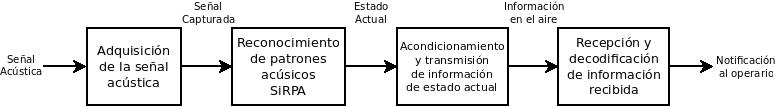
\includegraphics[width=\textwidth]{Nodo_RIS.jpeg}
\centering
\caption{Procesamiento realizado por cada nodo miembro de la RIS \cite{Jordanthesis}}
\label{nodoRIS}
\end{figure}


Interiorizando en la unidad de procesamiento, específicamente en el bloque denominado \textit{SiRPA} \footnote{SiRPA, es el acrónimo en español para Sistema de Reconocimiento de Patrones Acústicos}, este sigue una estructura estándar de un sistema de reconocimiento de patrones, el cual se compone de un bloque de preprocesado, una etapa de identificación/extracción de características fundamentales y un bloque de clasificación.

El preproceso consiste en acondicionar la señal analógica, en síntesis se refiere a normalizar y digitalizar la señal acústica. El bloque de identificación está compuesto por una batería de filtros, un estimador de energía, un reductor de dimensiones y un árbol clasificador. En el banco de filtros el espectro de la señal acústica se separa en 8 bandas distintas y luego se estima la energía a cada banda.

Mediante una transformación lineal, el reductor de dimensiones proyecta la salida del estimador de energía, que se encuentra en un espacio de ocho dimensiones, a un espacio de tres dimensiones. Según lo predice la \textit{maldición de dimensionalidad}, el conjunto de símbolos necesarios para describir de manera adecuada las observaciones realizadas es tres órdenes de magnitud superior si se emplea un espacio de ocho dimensiones en comparación a uno de tres. También tiene relación respecto a. \cite{NeuralNetworks, Jordanthesis}

El árbol binario o generador de símbolos, permite ubicar el centroide mas cercano a un patrón de entrada de tres dimensiones, para ello se utiliza la distancia L1 o Manhattan. Consecuentemente, los símbolos discretos se generan asociando estos, a las trayectorias continuas en el espacio del vector tridimensional de entrada, que describe la señal acústica en un determinado instante. El árbol binario genera un alfabeto de 32 símbolos discretos. \cite{IEEE_Panama, TDS, Jcardenas, EmbededTech}

Por último, encontramos la etapa de clasificación, encargada de calcular la probabilidad de que un conjunto de símbolos de entrada, formen parte de una señal acústica, de acuerdo con las categorías: bosque, motosierra o disparo. En este bloque, se utiliza un clasificador basado en la técnica de modelos ocultos de Markov (HMM). En la figura \ref{sirpa} se muestra un diagrama de bloques ilustrando como funciona internamente el SiRPA.

\begin{figure}[h]
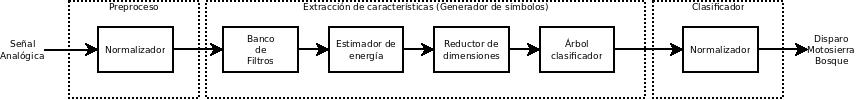
\includegraphics[width=\textwidth]{SiRPA.jpeg}
\centering
\caption{Diagrama de bloques del Sistema de Reconocimiento de Patrones Acústicos \cite{Carlosthesis}}
\label{sirpa}
\end{figure}


\section{Descripción del problema y justificación}

Como fue mencionado en el apartado anterior, países como Costa Rica ven amenazados sus recursos naturales por actividades ilegales como la caza furtiva y la tala. La tutela de los recursos naturales por parte del Estado es difícil, los bosques y los grandes mamíferos ven amenazada su conservación. En respuesta a esta situación la escuela de Ingeniería Electrónica del Instituto Tecnológico de Costa Rica, a través del \textit{DCILab} \footnote{DCILab: Laboratorio de Diseño de Circuitos Integrados} plantea una solución mediante un dispositivo electrónico de bajo consumo energético, capaz de reconocer sonidos como disparos de armas de fuego y motosierras. Esta iniciativa da a luz al proyecto SiRPA el cual pretende fabricar un \textit{ASIC} \footnote{ASIC es el acrónimo en inglés para: Circuito Integrado de Aplicación Especial... Se invita al lector a consultar un diccionario de términos electrónicos diccionario de términos electrónicos} con el fin de detectar la tala y caza ilegal en bosques, mediante el procesamiento digital de señales acústicas.

Luego de muchas etapas iterativas en el diseño del \textit{SiRPA}, el proyecto se encuentra codificado en un lenguaje de descripción de hardware (\textit{HDL}). Se han efectuado pruebas usando plataformas de sistemas embebidos como \textit{Beagle Boards} y textit{FPGAs} \footnotetext{Una FPGA (del inglés Field Programmable Gate Array) es un dispositivo electrónico que contiene bloques de lógica y electrónica digital que puede ser reconfigurada “in situ” mediante un lenguaje de descripción de hardware.} para la validación del diseño, se han publicado algunos papers al respecto, y se ha demostrado la viabilidad del proyecto, por lo que compete continuar la labor de
implementar la codificación \textit{HDL} a su etapa final, la cual consiste en la síntesis de los módulos
descritos en HDL sobre un chip de silicio.

Durante el 2014 el \textit{DCILab} contó con el apoyo del ingeniero argentino Dr. Juan Agustín Rodríguez, quien desarrolló un flujo de diseño digital sobre las herramientas de software Synopsys que implementan los módulos en HDL del \textit{SiRPA} al silicio para el circuito integrado. El trabajo del Dr.Rodríguez quedó incompleto y el \textit{SiRPA} no ha podido ser fabricado. Es por ello que el \textit{DCILab} requiere terminar el trabajo empezado por el Dr. Rodríguez e integrar la parte final del \textit{SiRPA}, que consiste en un microprocesador desarrollado por el Ing. M.Sc. Carlos Salazar García, para así dejar todo el proyecto \textit{SiRPA} depurado y listo para su fabricación. Además el \textit{DCILab} está interesado en que dicho proceso de síntesis quede documentado y se establezca una estructura de diseño digital genérica, capaz de ser adaptada para futuros proyectos.

Los investigadores del \textit{DCILab} logran fabricar sus circuitos integrados mediante el servicio de
“Obleas Multi-Proyectos” de \textit{MOSIS} \footnote{MOSIS (Metal Oxide Semiconductor Implementation Service): es un servicio que facilita servicios para la fabricación de circuitos integrados, como tal no es una fábrica, sólo un facilitador de tecnologías de fabricación.}. Este servicio lo brinda el Instituto de Ciencias de la
Información de la Universidad del Sur de California (USC). MOSIS consiste en un proyecto que ofrece
la opción para que pequeños diseñadores independientes, y instituciones académicas puedan fabricar
sus proyectos a un costo accesible y en una tecnología que se ajuste a sus requerimientos. \cite{website:mosis}

\section{Síntesis del problema}
El proyecto \textit{SiRPA} se encuentra inconcluso y el \textit{DCILab} requiere de una persona con conocimientos en microelectrónica capaz de someter los componentes del \textit{SiRPA} a un flujo de diseño \textit{ASIC}, y fabricar un prototipo \textit{SoC}.

\section{Enfoque de la solución}

\subsection{Generalidades de la solución}

Dado que se requiere diseñar un circuito integrado digital que parte de una codificación \textit{HDL}, es necesario desarrollar una jerarquía de diseño digital que permita realizar el layout de los módulos descritos en \textit{HDL}, por lo que se necesita de una herramienta de software especializada para tal fin. \textit{Design-Compiler} e \textit{IC-Compiler} son herramientas interactivas de \textit{Synopsys} que le permiten al usuario controlar el desarrollo del circuito integrado sobre el silicio, definiendo las características físicas como: conexión eléctrica, distribución espacial y física, limitaciones espaciales y sus implicaciones electromagnéticas para que su posterior fabricación e implementación física sean exitosas.

El proceso de diseño de un circuito integrado es lento, tedioso, y tiene un componente iterativo, esto implica que toma de algún tiempo para que un ingeniero se familiarice con el flujo de diseño, es por ello que aparte de crear el flujo de diseño de un chip sobre la herramientas, es conveniente establecer para futuros proyectos, una estructura de archivos y \textit{\textbf{scripts}}, propios de las herramientas de \textit{Synopsys}, para así facilitar el diseño y rediseño de proyectos futuros del \textit{DCILab}. Como comprobación de la efectividad del flujo de diseño digital anteriormente mencionado, deberán someterse los componentes del \textit{ASP} mediante las herramientas de  \textit{Synopsys}, para su posible fabricación a futuro, y establecer una documentación oportuna para agilizar el trabajo, de los colabores del \textit{DCILab} en cuanto a síntesis sobre silicio respecta.

\subsection{Síntesis de la solución}
Establecido el panorama anterior, la solución consiste en desarrollar una jerarquía de flujo de diseño digital en las herramientas de \textit{Synopsys}, que permita someter los componentes del \textit{SiRPA} al proceso de síntesis al silicio, según las reglas de diseño del proceso de fabricación de IBM: cmrf8 (IBM013), que es la tecnología a la cual
tiene acceso el \textit{DCILab}, y así contar con el proyecto \textit{SiRPA} completo hasta la última etapa previa a su fabricación que será realizada por \textit{MOSIS} en un futuro.
Cabe destacar que la índole del proyecto y las restricciones del laboratorio en términos de licencias de software solamente permiten una opción de \textit{EDA} \footnote{EDA: Electronic Design Automation. Software usado en la síntesis de circuitos integrados}, la cual es \textit{Synopsys}.

\section{Trabajos Anteriores}

\textit{SiRPA} es un proyecto de investigación que ha sido explorado y analizado desde diversas perspectivas de solución cada investigador ha dado forma a cada etapa que componen el sistema. Tanto a nivel de software como a nivel de hardware, los aportes incluyen desde propuestas de diseño, implementación, mejoras o rediseño de etapas que han presentado problemas. Entre estos trabajos se encuentran los siguientes:

\begin{itemize}

\item {En \cite{MSaenz}, se efectuó la primera prueba de concepto para evaluar la viabilidad de implementar el SiRPA. Se empleó el software MATLAB, para generar un modelo de alto nivel cuyo objetivo fue el análisis de las señales acústicas y se desarrolló una etapa de identificación de características utilizando la teoría de onditas (wavelets en ingles). Este trabajo constituye la primer referencia del sistema. La estrategia de extracción de características mediante onditas fue descartada posteriormente}

\item {En \cite{Esalas}, se implementó el \textit{SiRPA} en una \textit{FPGA} utilizando el lenguaje de descripción de hardware \textit{VHDL}, de este trabajo se establece que el uso de un banco de filtros utilizando una misma unidad de filtro para cada una de las ocho bandas constituye una metodología de clasificación idónea para los requerimientos de hardware del \textit{SiRPA}. Es en este trabajo donde se intenta implementar por primera vez el algoritmo de \textit{HMM} en hardware mediante un MAP (del ingles Matrix and Arrays Processor), el cual consiste una estructura digital cuya arquitectura se optimiza de acuerdo con la ejecución de operaciones en punto flotante en 32 bits de forma combinacional.}

\item {En \cite{Msequeira}, se desarrolló un módulo reductor de dimensiones mediante la estrategia de transformación lineal, fundamentada en el algoritmo de discriminantes de Fisher. Este módulo permite transformar un espacio de 8 dimensiones en un espacio de 3 dimensiones, que implica mayor facilidad en la clasificación de señales acústicas y ahorro energético, al disminuir la densidad de hardware.}

\item {En \cite{Jcardenas}, se desarrolló la herramienta HMMSoft que consiste en un software de alto nivel (lenguaje C/C++) con interfaz gráfica, capaz de realizar el entrenamiento del algoritmo de \textit{HMM} utilizado por el clasificador. Esta aplicación permite identificar características de patrones acústicos lo cual contribuye a validar el reconocimiento de un audio en particular. Esta herramienta representa un hito considerable ya que mediante ella, es posible establecer un marco de referencia para la verificación funcional del sistema.}

\item {En el trabajo de \cite{Jordanthesis}, se realizó la síntesis de la sección de extracción de los patrones acústicos y entrenamiento a partir de conjuntos de datos de audio similares a los que se esperara detectar. El proceso de extracción mencionado fue integrado a la aplicación HMMSoft \cite{Jcardenas}. Consecuentemente el proyecto \textit{SiRPA} fue modelado en el lenguaje C, e implementado en un sistema embebido (BeagleBoard xM)  \cite{website:beagleboard} y usando la herramienta HMMSoft además del modelo en C del \textit{SiRPA} se desarrolló el primer modelo de verficación para \textit{SiRPA}} 

\item {En \cite{Lalfaro}, se implementaron los módulos de hardware del reductor de dimensiones, generador de símbolos y una unidad de \textit{HMM} en \textit{Verilog}. Partiendo de la estructura de la unidad \textit{HMM} desarrollada por \cite{Jordanthesis} para el sistema embebido, en \cite{Lalfaro} se propone implemetar la unidad mediante una máquina microprogramada. Posteriormente al realizar pruebas sobre una FPGA, se observó que los resultados divergen de lo esperado según el modelo de \cite{Jordanthesis} y por tanto clasificar los patrones acústicos correctamente es imposible. Según expone \cite{Carlosthesis} el hardware presenta problemas de cálculo ya que los resultados tienden a cero rápidamente debido a que en \cite{Lalfaro}, no se consideran los problemas de escalamiento que se describen ámpliamente en \cite{LRabiner}.}

\item {En \cite{Mau}, se expone la verificación funcional de los módulos descritos en hardware (textit{HMM}) que conforman el SiRPA.}

\item {En \cite{mio}, se toma como punto de partida el trabajo de \cite{Esalas} y se rediseñó la unidad contemplando efectos de submuestreo. De acuerdo con un analisis del bloque de reducción de dimensiones elaborado en \cite{Lalfaro} se estableció la necesidad de aumentar el formato de palabra de 16 a 24 bits. Por lo tanto se integraron además todos los bloques para formar la etapa de identificación o extracción de características. Finalmente, se evaluó la funcionalidad de esta etapa, tomando como referencia dorada el trabajo realizado en \cite{Jordanthesis}.}

\item {En \cite{Carlosthesis} se expone la necesidad de implementar la unidad de clasificación \textit{HMM} mediante un microprocesador de aplicación específica ya que durante la experimentación en \cite{mio} se determinó que la unidad \textit{HMM} implementada en \cite{Lalfaro} no era correcta.}

\end{itemize}

\section{Objetivos}

\subsection{Meta}

Desarrollar un sistema de detección de disparos de armas de fuego, motosierras y otras actividades ilegales en un bosque, que esté implementado en un circuito integrado de bajo consumo energético.

\subsection{Objetivo General}

Implementar un microprocesador de aplicación específica en una tecnología CMOS de 0,13 micrómetros para posteriormente ser integrado al proyecto SiRPA.


\subsection{Objetivos Específicos}

\begin{itemize}

\item{Diseñar una jerarquía de scripting \footnote{En informática un script es un archivo que contiene un conjunto de órdenes e instrucciones, las cuales ejecutan una función, ya sea en un lenguaje de programación o una herramienta de software. Se invita al lector a consultar un diccionario de términos de computación} que implemente el flujo de síntesis y simulaciones {"Post Colocado y Enrutamiento"} (Place\&Route), para optimizar el tiempo del proceso de diseño para futuros proyectos.}

\item {Sintetizar lógicamente de manera correcta los módulos RTL del Microprocesador de Aplicación Específica (ASP) sobre celdas estándar de una tecnología CMOS 0,13.}

\item {Sintetizar físicamente de manera correcta la unidad aritmética del microprocesador y la memoria de programa del microprocesador ASP sobre la tecnología CMOS 0,13}

\end{itemize}
%%% Local Variables: 
%%% mode: latex
%%% TeX-master: "main"
%%% End: 

  \chapter{Marco Teórico}
\label{ch:marco}
\subsection*{Diseño de ASICs}

{Esta tesis no pretende exponer el proceso de fabricación de un circuito integrado, esa información puede encontrarse en un libro de texto sobre diseño VLSI; sin embargo, en las secciones siguientes se expondrá brevemente, la metodología que se esta usando para que a futuro se pueda llevar a cabo la implementación de un sistema sobre un dado de silicio (silicon dice), entendiendo por dado el espacio que el sistema propuesto ocupará sobre la oblea de silicio, al final del proceso de fabricación.

Comercialmente la manufacturación de ASICs no es rentable para aplicaciones de envergadura pequeña, ya que un proceso de fabricación fácilmente alcanza los millones de dolares, si se tiene una proyección comercial baja o nula esta opción queda descartada, la forma más fácil de implementar un diseño en un chip sería venderle la idea o diseño a un fabricante.

No obstante, venderle la idea o diseño a un fabricante implica revelar información sensible sobre el producto y el fabricante probablemente este trabajando con su competencia por lo que revelarle su trabajo a un fabricante tampoco es la mejor opción.

Sin embargo, es posible hacer el proceso de diseño, posteriormente generar un archivo que contenga toda la información estrictamente necesaria para que el fabricante pueda implementar el diseño sobre el chip, sin tener revelar la información sensible que se pretende proteger.

Esta suele ser la opción más viable para los pequeños investigadores; no obstante, existe la problemática que este tipo de servicio alcanza precios muy elevados sobre todo si se pretende emplear los procesos más modernos y las tecnologías de vanguardia.

En respuesta a la problemática de no tener suficientes fondos para concretar una fabricación, existe el servicio de óbleas multiproposito de la universidad de Berkeley (\textit{MOSIS}).

La funcionalidad de implementar sistemas sobre chips (SoC) tiene grandes ventajas respecto a sistemas embebidos o implementados mediante software de alto nivel.

En primera instancia producir un sistema en un circuito integrado representa una mejor protección para los derechos intelectuales, pues su contenido difícilmente es reproducible. Un circuito integrado presenta enormes facilidades de portabilidad debido a su tamaño y su consumo energético. Lo cual es el principal objetivo del proyecto: "Sonidos Ilegales".

\subsection*{Sobre la tecnología de fabricación}

Para el presente proyecto se hace uso de la tecnología de IBM CMOS8RF (CMRF8SF), esta tecnología cuenta con una alta densidad de lógica CMOS de  0.13 $\mu$m destinada a aplicaciones de señal mixta, en ámbitos asociados al procesamiento analógico y de radio frecuencia . Entre las generalidades del proceso, cabe destacar que cuenta con 8 capas de metal, y la tensión $V_{DD}$ de los dispositivos se encuentra en un rango de 1.2 V a 1.5 V.\\

\section{Tipos de diseño circuitos integrados digitales}

La clasificación del diseño de circuitos integrados se puede apreciar en el esquema de la figura \ref{ICs}.

\begin{figure}[h]
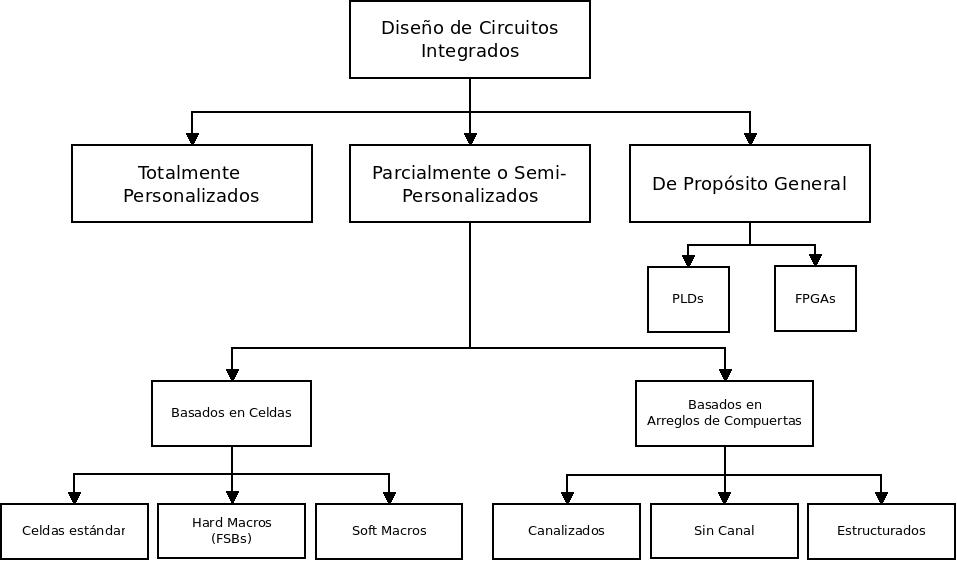
\includegraphics[width=\textwidth]{Tipos_de_ICs.jpeg}
\centering
\caption{Tipos de Diseño de Circuitos Integrados}
\label{ICs}
\end{figure}
Como podemos observar el diseño de circuitos integrados (De aquí en adelante ICs\footnote{ICs: acrónimo en inglés para circuitos integrados}) se puede clasificar a grosso modo en 3 tipos principales:

\subsection{\textbf{ICs totalmente personalizados}}

En esta metodología de trabajo los diseñadores generan todas las celdas lógicas de acuerdo con las necesidades tiene el diseño que se pretende realizar, esto contempla desde la concepción funcional, lógica y física de cada celda. También se desarrollan las máscaras necesarias para la fabricación del chip sobre la oblea de silicio.

Empresas como Intel son un buen ejemplo de industrias dedicadas al desarrollo de circuitos integrados totalmente personalizados, aquí los ingenieros invierten enormes cantidades de tiempo maximizando el aprovechamiento de cada micrómetro cuadrado disponible en el dado, lo que les permite incluir circuitos analógicos, optimizar celdas de memoria e incluso contemplar y mejorar la eficiencia mecánica de las estructuras de conexión y ubicación de los componentes del chip.

Sin duda la metodología más costosa de todas. No obstante, la respuesta adecuada si el diseñador necesita de unidades (celdas) más eficientes en términos energéticos y velocidad, de las que es capaz de encontrar en una biblioteca de celdas existentes. Es comúnmente utilizada por empresas dedicadas a la innovación y el desarrollo tecnológico.

\subsection{\textbf{ICs programables}}

Estos consisten en dispositivos lógicos programables (PLDs), que son circuitos integrados con configuraciones estándar, predeterminadas. Podemos encontrarlos en algunos ASICs para permitir la personalización de algunas funciones puntuales, es por ello que aunque sean estructuras prediseñadas y flexibles, son consideradas como una rama del diseño de ICs.

\subsection{\textbf{ICs semipersonalizados}}

Son aquellos ICs para los cuales existe una biblioteca de celdas estándar y posiblemente todas las mascaras de diseño están disponibles. El uso de bibliotecas de celdas prediseñadas hace el diseño más fácil. Está metodología de diseño se subdivide en dos partes:

\subsubsection{Basado en arreglos de compuertas}

En este tipo de diseño los transistores se encuentran predefinidos en un patrón dado sobre en la oblea de silicio, este patrón se conoce como arreglo base y a los elementos más pequeños se los conoce como celdas base o celdas primitivas.

En esta técnica el diseñador únicamente define la interconexión de las celdas usando para ello máscaras personalizadas. Así el diseñador escoge de entre una basta biblioteca de celdas prediseñadas y precaracterizadas. Las celdas lógicas suelen ser denominadas como macros. La razón de esto se debe a que el layout \footnote{En este contexto, refiere al anglisismo asociado al concepto de diseño físico} de la celda base es el mismo para cada celda lógica y únicamente se personaliza la interconexión y el enrutado dentro de las celdas y con las celdas adyacentes, de manera similar a un macro de software.

Existen subcategorias del uso de esta técnica, pero esa información excede el alcance de esta tésis, por lo que no serán expuestas. Se invita al lector a considerar una bibliografía pertinente \cite{book:johnM1997,book:barrK2006}

\subsubsection{Basado en celdas estándar}

Un circuito integrado basado en celdas estándar usa celdas lógicas prediseñadas como compuertas "Y", "O", "Flip Flops", "Multiplexores", etc... Estas celdas se conocen como celdas estándar.

Suele usarse el término \textit{CBIC} (pronunciado si-bik) para esta categoría. El área de ubicación de las celdas estándar en un \textit{CBIC}, se construye en hileras, de manera similar a una pared de ladrillos, las celdas estándar pueden y suelen ser utilizadas en conjunto a microcontroladores, o microprocesadores, conocidos como "Mega celdas". Este término también se emplea para bloques totalmente personalizados, y suelen ser denominados como: "Macros a Nivel de Sistema (SLMs)", "Mega Funciones", "Bloques Fijos", o "Bloques Funcionales Estándar (FSBs)".

En esta metodología es diseñador define únicamente la colocación y el enrutado (interconexión entre celdas estándar) de las celdas estándar; sin embargo, estás pueden ser colocadas libremente en el área disponible del dado. Esto implica que las máscaras de fabricación en un \textit{CBIC} son únicas para cada cliente.

Usar \textit{CBICs} tiene enormes ventajas ya que permite hacer diseños más flexibles y optimizarlos en términos de aprovechamiento de área, velocidad o consumo energético. Adicionalmente las bibliotecas de celdas estándar suelen ofrecer las mismas celdas estándar prediseñadas para cumplir distintas las expectativas de desempeño, enfocadas a tamaño, velocidad o energía.

Las principales desventajas consisten en que el tiempo necesario para el diseño suele ser elevado, debe comprarse una biblioteca de celdas estándar, y se está sujeto a las restricciones de esta, y finalmente las máscaras de fabricación serán nuevas con cada nuevo diseño o versión de diseño, lo cual implica tiempo adicional, además de costos adicionales por parte del fabricante.

La información de esta sección se tomó a partir de las fuentes \cite{book:raj2008,book:johnM1997,book:raj2008}

\section{Flujo de diseño digital para el diseño de circuitos integrados digitales}

Dada la complejidad en el proceso de diseño de circuitos integrados, es imperativo llevar a cabo un diseño estructurado, que use los principios de jerarquización, modularidad, regularidad y localidad para manejar la complejidad del diseño.

El diseño digital VLSI suele ser particionado en 5 niveles de abstracción: diseño de arquitecturas, diseño de microarquitecturas, diseño lógico, diseño de circuitos y diseño físico. Estas etapas son ejecutadas en paralelo, y en muchas ocasiones son depedientes entre si.

Una manera alternativa de analizar el diseño estructurado es mediante el "diagrama Y" mostrado en la figura \ref{Ychart}. 

\begin{figure}[h]
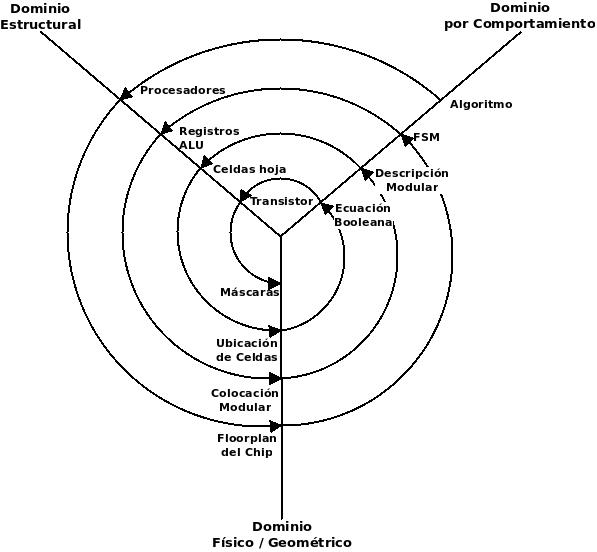
\includegraphics[width=\textwidth]{Gajski_Y_Chart.jpeg}
\centering
\caption{Diagrama de Gajski. Espiral que ilustra el flujo digital de diseño de circuitos integrados y cuyas arístas establecen los ámbitos por los que debe atravesar el diseño. Figura de autoría propia, basada en la reproducción de \cite{book:weste2005}, créditos a sus respectivos dueños}
\label{Ychart}
\end{figure}

El diagrama de Gajski o diagrama Y, permite entender el concepto de abstracción en el diseño digital, pues se parte desde un concepto general de diseño y al interiorizar en el diagrama se desvelan las etapas que llevan hasta la fabricación correcta del circuito integrado.

El dominio por comportamiento describe qué hace el sistema, seguidamente en el dominio estructural, el cual expone la interconexión de los módulos capaces de realizar el comportamiento deseado, eventualmente a los niveles de abstracción más bajos donde se describen las compuertas individuales y las conexiones entre los transistores que las componen. Finalmente en cada nivel de abstracción del dominio físico se explica como se construye físicamente ese nivel de abstracción, en los niveles más altos se considera el diseño del floorplan del chip, donde en esencia se , y consecuentemente al internarse en los niveles más profundos se describen la geometría actual de cada transistor individual.

El proceso de diseño puede verse como la transformación desde un dominio hacia otro manteniendo la equivalencia de los dominios. Las descripciones por comportamiento se transforman en descripciones estructurales y estas a su vez son transformadas en descripciones físicas. Cada transformación es validada, ya sea manualmente o mediante herramientas automatizadas. La especificación jerárquica de cada dominio y sucesivamente detallando sus niveles de abstracción es lo que permite diseñar grandes sistemas. 

La razón para describir en detalle los niveles de abstracción y los respectivos dominios es para definir un proceso de diseño en el cual la función final del sistema es capaz de rastrearse hasta la descripción por comportamiento inicial.

El diagrama Y muestra las transformaciones entre cada dominio y las variaciones entre los niveles de abstracción. El flujo de diseño procede desde los anillos exteriores hacia los interiores, profundizando en niveles de abstracción cada vez más complejos, de acuerdo a una jerarquía establecida.

El apartado anterior corresponde a una libre interpretación de la sección 1.6 de \cite{book:weste2005}.

\subsection{Generalidades del flujo de diseño digital}
\label{sec:gen_d_flow}
\begin{figure}[t]
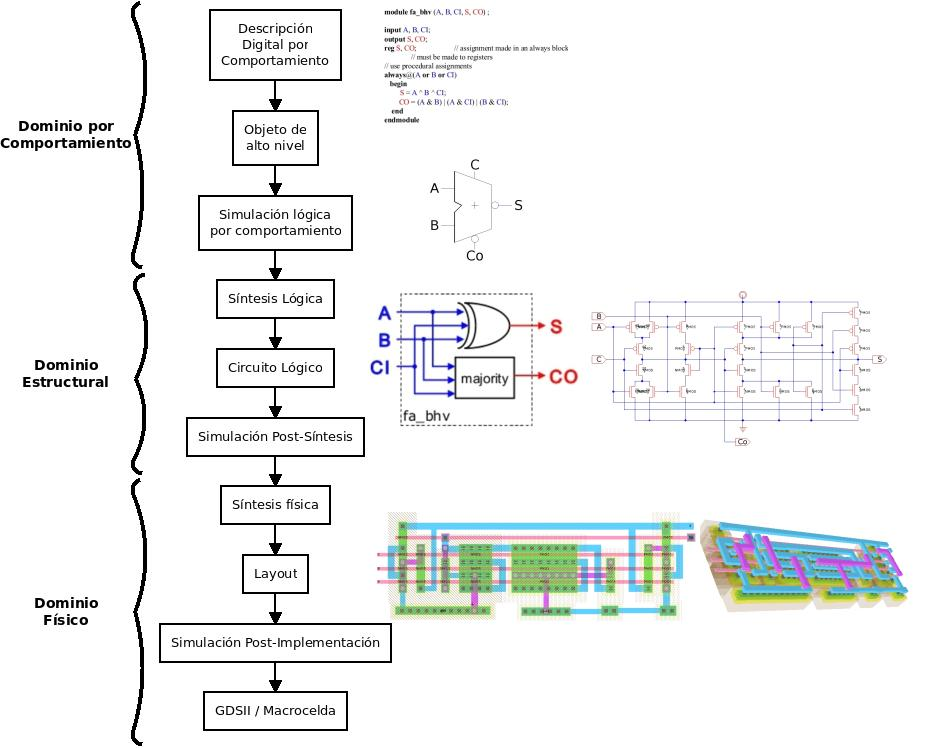
\includegraphics[width=\textwidth]{Flujo_Digital.jpeg}
\centering
\caption{Esquema representativo e ilustrativo del flujo de diseño de circuitos integrados digitales}
\label{Dflow1}
\end{figure}

Como se mencionó en el apartado anterior, el diseño comienza a dar sus pasos en cuanto es concebida una función o proceso y su comportamiento ha sido modelada en un algoritmo, ya sea secuencial, concurrente o una mezcla de ambos. Este algoritmo se traduce a un lenguaje estandarizado, el cual en el caso de los circuitos integrados digitales corresponde a un \textit{HDL}, que en términos concretos es la descripción digital del circuito integrado o el modelo digital.

Partiendo del modelo digital se puede hacer una verificación de comportamiento, que en términos técnicos se denomina simulación lógica, el modelo digital no es más que un objeto de alto nivel capaz de emular el comportamiento deseado. Su utilidad es poca para el diseñador, ya que no provee datos sobre el desempeño del diseño, únicamente provee 
información a nivel de comportamiento; sin embargo, es el punto de partida en el flujo de diseño.

Una vez que la simulación lógica es satisfactoria, se procede a usar el modelo por comportamiento y asociar los módulos descritos en él, con unidades lógicas provistas de características de retardos (sincronización de señales), consumo energético, y área, las cuales se encuentran en la biblioteca de la tecnología que se usará en la fabricación. A este proceso se le conoce como síntesis lógica, y genera una base de datos que contiene datos de las celdas estándar y las conexiones entre ellas para ejecutar las funciones abstraídas del modelo de comportamiento.

La base de datos creada en el proceso de síntesis permite generar un nuevo modelo codificado en \textit{HDL} y una primera aproximación del desempeño de los módulos diseñados, i.e. un modelo con la información sobre los retardos de propagación de las señales en las celdas y entre las mismas, generar un presupuesto de la energía disipada y el área necesaria para ubicar las celdas usadas. Este nuevo modelo, denominado como modelo post-síntesis nuevamente es simulado con el mismo arreglo o banco de pruebas usado en la simulación por comportamiento.

La simulación post-síntesis permite observar el retardo de propagación de las señales, y confirmar si las expectativas de sincronización son alcanzadas, también permite verificar si los datos son generados en los plazos necesarios, y poder garantizar una funcionalidad correcta de los módulos y el diseño en lo concerniente al desempeño de las celdas estándar. 

Cuando los resultados obtenidos en la síntesis lógica y la simulación respectiva sean satisfactorios, se toma el modelo post-síntesis y se usa esta información para empezar con el floorplan del chip. Las celdas estándar son invocadas a un área determinada, y posteriormente se establecen las conexiones que permiten implementar los módulos abstraídos en la primera etapa del diseño (el modelo de comportamiento). Este proceso recibe el nombre de síntesis física o implementación física, en esta tésis se usará la palabra síntesis para referirse a la síntesis lógica, y la palabra implementación será usada para referirse a la síntesis física.

Una vez hecho lo anterior, se genera una nueva base de datos, la cual tendrá información más precisa sobre el diseño, nuevamente en términos de sincronización de señales, consumo energético y aprovechamiento de área, incluyendo los retardos debido a los efectos parasíticos, la distancia que debe recorrer una señal al conectarse de una celda a otra o un puerto, etc, las perdidas resistivas del alambrado, entre otros efectos que serán expuestos más adelante.

Nuevamente se genera una base de datos con la información del colocamiento y el enrutado (Place\&Route), así como los efectos sobre el tiempo de propagación de las señales, mediante la esta base de datos se generan, un modelo codificado en \textit{HDL} para la verificación del diseño, y el modelo de los efectos sobre el temporizado y la sincronización de las señales. En esta etapa es posible obtener una respuesta más precisa del diseño. Al igual que en la etapa anterior también se crean reportes de consumo energético, aprovechamiento de área, calidad de resultados, etc.

Cuando una simulación post-implementación es satisfactoria se procede a dar por concluído el flujo, y a continuación se establecen 2 panorámas.

En el primer caso nuestro diseño está completo por lo que se procede a compilar la base de datos en un archivo estándar para condensar la información necesaria para el fabricante, y este valorará si el diseño tiene probabilidades altas de ser fabricado con éxito, siendo así la información suministrada será usada para desarrollar las máscaras necesarias para la construcción del chip.

En el segundo escenario consiste en que el diseño en el que se ha estado trabajando no es el producto final, sino que forma parte de otro diseño más complejo y grande, el cual aún no se haya terminado, en ese caso la base de datos servirá para generar una macro celda que será utilizada en diseños posteriores.

En la figura \ref{Dflow1} se aprecia un resumen gráfico de la explicación anterior.

\subsection{Flujo de diseño digital en las herramientas de Synopsys}

Synopsys es una empresa que brinda herramientas de diseño asistido por computadora (CAD), para la automatización de procesos en el diseño de circuitos integrados. El flujo de diseño digital suele ser similar independientemente del proveedor de las herramientas; sin embargo, esta tesis gira entorno a los softwares de Synopsys, por lo que se expondrá la metodología de diseño usando este proveedor.

\subsection{Front End}

\begin{figure}[h]
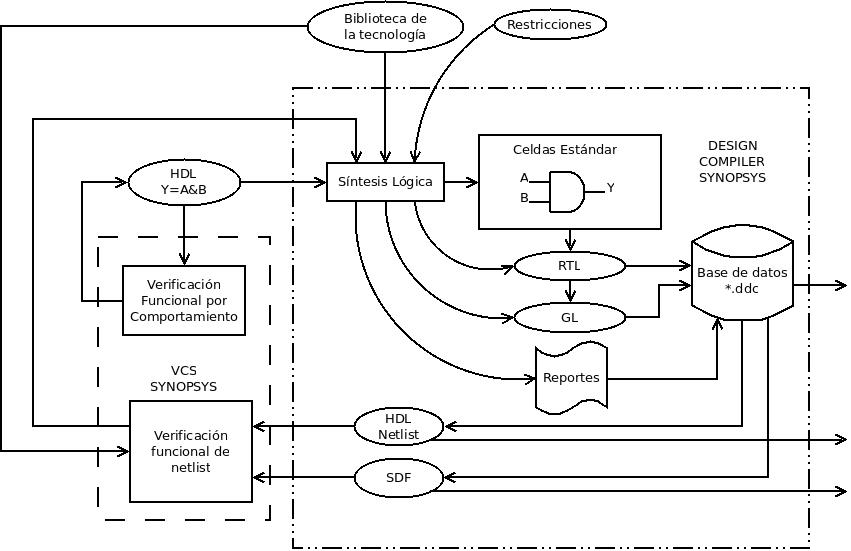
\includegraphics[width=\textwidth]{Front_End.jpeg}
\centering
\caption{Esquema ilustrativo del flujo de diseño de circuitos integrados digitales, enfocado a las herramientas de síntesis lógica, en esencia las herramientas de Front End}
\label{fe}
\end{figure}


El término "Front End", es un concepto en inglés asociado a la jerga del desarrollo de software, y significa interfaz; sin embargo, en el caso del diseño de circuitos integrados, no se generan softwares y tampoco interfaces. Una traducción más literal, y por lo tanto, menos elegante del concepto sería "Fachada", y es en esencia con lo que el diseñador interactúa en la primer etapa del diseño.

Al decir que el diseñador interactúa con una fachada, se debe entender que el diseñador trabaja con el cascarón de un elemento que intrínsecamente no es circuito electrónico como tal, si no un modelo abstracto que presenta un comportamiento de causa efecto, el cual, naturalmente, es acorde a la semántica de la lógica digital, o lógica binaria. Recurriendo nuevamente a la jerga del software, podemos entender el front end o fachada como aquello relacionado con un objeto de alto nivel, que ofrece un vector de respuestas de acuerdo con la dinámica de un vector de estímulos.

El diseñador comienza a acercarse al diseño del circuito integrado, considerando y definiendo los aspectos principales de la fachada. Retomando el diagrama de Gajski (figura \ref{Ychart}), el proceso de "Front-End" consiste en la transición del modelo de comportamiento a un modelo estructurado, que se asocia con las funciones de las celdas estándar ofrecidas por la tecnología y el fabricante.

Condensando lo anterior, las herramientas de "Front-End" de un proveedor, son aquellas que ejecutan o facilitan el proceso de síntesis lógica en el flujo digital del diseño de circuitos integrados. En el caso de "Synopsys", estas herramientas son principalmente "Design Compiler" y "VCS", existen otras herramientas adicionales asociadas a la familia de "Design Compiler", "VCS" y el "Shell" de "Design Compiler" son las principales y suelen ser suficientes.

En la figura \ref{fe} se aprecia un diagrama que ilustra como el proceso expuesto en la sección \ref{sec:gen_d_flow}, es implementado por las herramientas de "Synopsys" todos los procesos en el diseño de circuitos integrados tienen un componente iterativo, y en este diagrama vemos como antes de avanzar en el flujo, se atraviesa por etapas a las que se recurre con frecuencia, estas etapas son las simulaciones por comportamiento y post-síntesis. La depuración de la etapa de síntesis es esencial para garantizar el éxito final del proyecto, por lo que las simulaciones tienen una gran importancia.

Cómo se observa desde el diagrama de Gajski (figura \ref{Ychart}), las herramientas de "front end" traducen el diseño por comportamiento en modelos de altos nivel de circuitos digitales, aunque como tal no se trabajan con circuitos lógicos reales, y para efectos prácticos el diseñador nunca trabaja realmente con elementos lógicos y digitales, las herramientas proveen la virtualización del comportamiento diseñado, mediante una biblioteca de simulación, las celdas estándar abstraídas en el proceso de síntesis, se comportarán como un elemento de circuito digital real, de ahí que se pueda validar si la etapa de síntesis cumple las expectativas del diseñador.

\newpage
\subsection{Back End}

\begin{figure}[h]
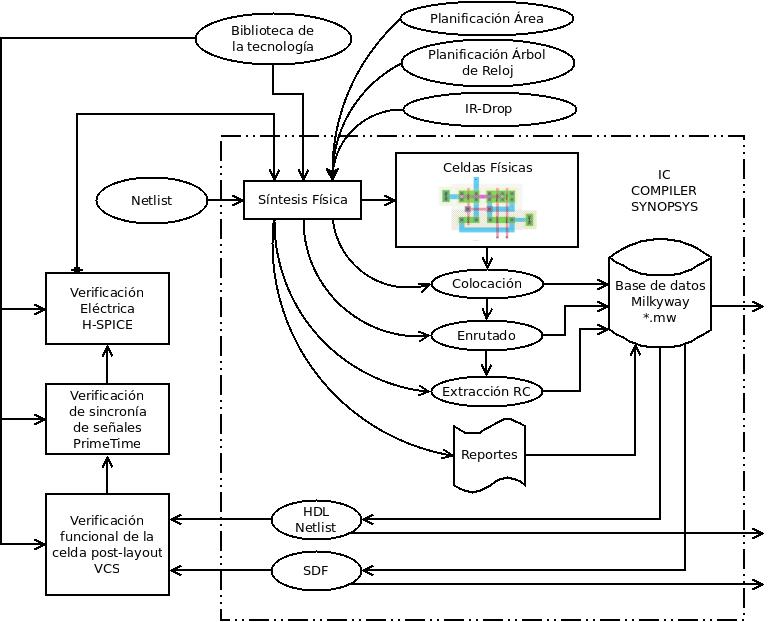
\includegraphics[width=\textwidth]{Back_End.jpeg}
\centering
\caption{Esquema ilustrativo del flujo de diseño de circuitos integrados digitales, enfocado a las herramientas de síntesis lógica, en esencia las herramientas de Front End}
\label{be}
\end{figure}

Se refiere a aquellos procedimientos relacionados con la constitución interna de un proyecto, nuevamente se emplea el anglicismo "Back End" para referirse a dichos procesos. No existe un concepto en español capaz de traducir el significado de esta palabra, pero se podría entender como todos aquellos aspectos ocultos al macro diseñador, entendiendo por oculto, una serie de elementos compuestos por elementos más simples hasta llegar a las unidades fundamentales de la electrónica moderna, i.e. transistores. Una analogía curiosa, y que ilustra bien esta situación es la de la muñeca matryoshka \cite{book:matryoshka}, cada muñeca contiene a otra muñeca más pequeña, y se interioriza así hasta alcanzar una pequeña muñeca que no contiene a ninguna otra.

En el proceso de diseño de circuitos integrados, semipersonalizados, y basados en celdas estándar, el diseñador no alcanza a trabajar directamente con transistores, o con los elementos que componen las celdas, si no, que da por hecho que las celdas estándar son funcionales y parte de ellas para generar nuevas macroceldas, y con las cuales se ejecutarán las funciones establecidas por el macromodelado del funcionamento del diseño.

En síntesis de lo anterior, el diseñador de "back end" trabaja con las etapas ocultas para los diseñadores de comportamiento, y síntesis del diseño, dónde los primeros establecen la semántica del diseño, y los segundos generan cajas negras que realizan las funciones descritas por sus antecesores, estas cajas negras manifiestan el comportamiento de una unidad electrónica real, en términos de consumo energético, área, y tiempos de propagación de señales, pero no dejan de ser modelos de alto nivel que no son circuitos electrónicos como tales, y es por ello que ha esta etapa se le denomina fachada.

En el proceso de "back end" las cajas negras abstraídas en el proceso de síntesis adquieren información más realista y equivalente a la de una celda física real. Esto podemos apreciarlo en la figura \ref{Dflow1} en el extremo derecho de la figura vemos como se muestran las etapas del flujo, en el dominio estructural, donde operan las herramientas de síntesis, aquí se muestran los bloques funcionales a nivel lógico. Al descender en el flujo expuesto en la misma figura, observamos la celda estándar que se abstrae del diseño estructurado, y su layout o implementación física, donde se aprecian los metales que interconectan las celdas y los transistores que componen las celdas.

Las herramientas de "back end" se encargan de facilitar el colocado y enrutado de las celdas estándar que se abstrajeron de la síntesis lógica. En el "back end" se asocia la base de datos post síntesis con la base de datos de la tecnología, invocando celdas físicas para generar un nuevo layout que implemente el diseño sintetizado. "Synopsys" cuenta con una herramienta llamada "IC Compiler", este software le permite al diseñador establecer los criterios de optimización del layout en términos de aprovechamiento de área, colocación selectiva para mejorar la eficiencia del consumo energético, sincronización de señales críticas, como lo es una señal de reloj, definir criterios de alambrado (enrutado) para sopesar las pérdidas resistivas, controlar fenómenos de electromigración y radiación o antena.





  \chapter{Flujo de Diseño Digital de Circuitos Integrados con las herramientas de Synopsys. Estructura de Scripting}
\label{ch:scripting}

A continuación se detalla la estructura propuesta para implementar un flujo de diseño de circuitos integrados, y se expone como fueron sometidos los módulos de un microprocesador ASP RISC-V, con el fin de demostrar la efectividad del flujo de diseño digital propuesto. Esta estructura está basada en el manual sobre el uso de las herramientas de Synopsys en el flujo de diseño de ASICs, del Instituto Tecnológico de Costa Rica \cite{FlujoJairo2016}.

La siguiente estructura dista considerablemente de la propuesta en \cite{FlujoJairo2016} y que a su vez está basada en el manual \cite{kommuru2009asic}. En estos trabajos las estructuras se basan en ejemplos simples con diseños \textit{HDL} relativamente pequeños. La siguiente estructura toma como premisa que se trabaja con diseños muy grandes por lo que se requiere de mayor eficiencia en la generación de las bases de datos y archivos necesarios para el diseño.

Dado que las herramientas EDA que se utilizan corren en "Linux", muchos de los scripts que se encuentran en esta estructura, hacen referencia a particularidades de este sistema operativo y no se describen en detalle pues abundar sobre el entorno "CentOS de Linux" esta fuera del objetivo de este proyecto, es por ello que se parte de la premisa que el lector cuenta con el conocimiento suficiente de este sistema operativo.

La primera propuesta de esta estructura fue desarrollada por el Dr. Juan Agustín Rodríguez y se tomó como referencia para desarrollar la que a continuación se expondrá. La estructura que se propone se basa en 3 principios muy relacionados con el mundo de desarrollo de software; sin embargo, apelan más a la experiencia práctica del Dr. Rodríguez y del aspirante que escribió este informe.

\begin{itemize}
\item {\textbf{Regularidad:}} {Este concepto se refiere a la uniformidad con la que los elementos desarrollados se ubican, dentro de la estructura de archivos y directorios, los cuales están basados en un principio o plan.

Esta estructura es "regular" en tanto presenta la misma morfología para los distintos directorios, esto quiere decir que aunque los directorios contienen archivos de distinta naturaleza, la mayoría presentan una jerarquía constante entre sí.}

\item {\textbf{Localidad:}} {Se refiere a usar archivos y directorios únicos, para evitar el manejo de múltiples versiones y múltiples rutas de acceso a archivos que en esencia son iguales, lo cual suele ser un problema cuando se debe involucrar a más personas en un proyecto.

La estructura presenta "localidad" en tanto los archivos fuente y las bases de datos generadas por los procesos de síntesis, únicamente residen en un único directorio y presentan sólo una ruta de acceso, no se generan copias de estos archivos en otros directorios, y la forma en que se accede a ellos es mediante punteros. Existen algunas excepciones a este principio; sin embargo, serán expuestas más adelante y se justificará el porqué de estos archivos.}

\item {\textbf{Continuidad:}} {La "continuidad" hace referencia a dos conceptos, el primero es sobre la capacidad de poder usar elementos en la estructura del flujo para rastrear el diseño en una etapa dada, hasta la etapa de origen que en este caso corresponde al modelo de comportamiento del diseño.

El segundo se relaciona con la capacidad de ser permanente, o en otras palabras tener la capacidad de degradarse con lentitud, es frecuente encontrar que entre diseñadores existan desacuerdos sobre la mejor forma de nombrar los archivos o la mejor manera de ubicarlos y realmente no es posible definir una estructura como la más eficiente o la estructura suprema, pues apela a muchos criterios subjetivos y relativos, tanto por parte de los diseñadores como por la naturaleza de los proyectos. 

Finalmente se afirma que la estructura es continua, ya que la navegación dentro de los directorios permite identificar de forma fácil e intuitiva, las distintas etapas del flujo, y mediante los scripts, y un conocimiento general del flujo descrito en la sección \ref{sec:gen_d_flow}, es posible ubicar los resultados de las distintas etapas y los archivos fuente que se fueron usados para generarlos (los resultados). Respecto a la parte de continuidad en el tiempo, se espera ofrecer una estructura lo suficientemente elegante y práctica para que pueda seguir siendo utilizada en futuros proyectos y que los diseñadores que los enfrenten puedan sentirse cómodos con ella.}

\end{itemize}

\section{Estructura de directorios y archivos}

\begin{figure}[h]
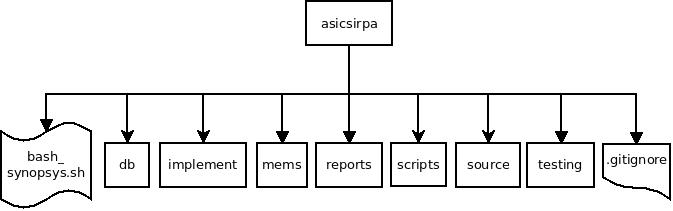
\includegraphics[width=\textwidth]{estructura_1.jpeg}
\centering
\caption{Esquema de la jerarquía de directorios y archivos para implementar el flujo de diseño digital. El archivo .gitignore es un archivo oculto, contiene información para que el sistema de control de versiones opere de forma personalizada, carece de relevancia para la estructura del flujo; sin embargo, permite mantener un repositorio más ordenado. \cite{website:gitignore, website:cvs}}
\label{directorios}
\end{figure}


\begin{figure}[h]
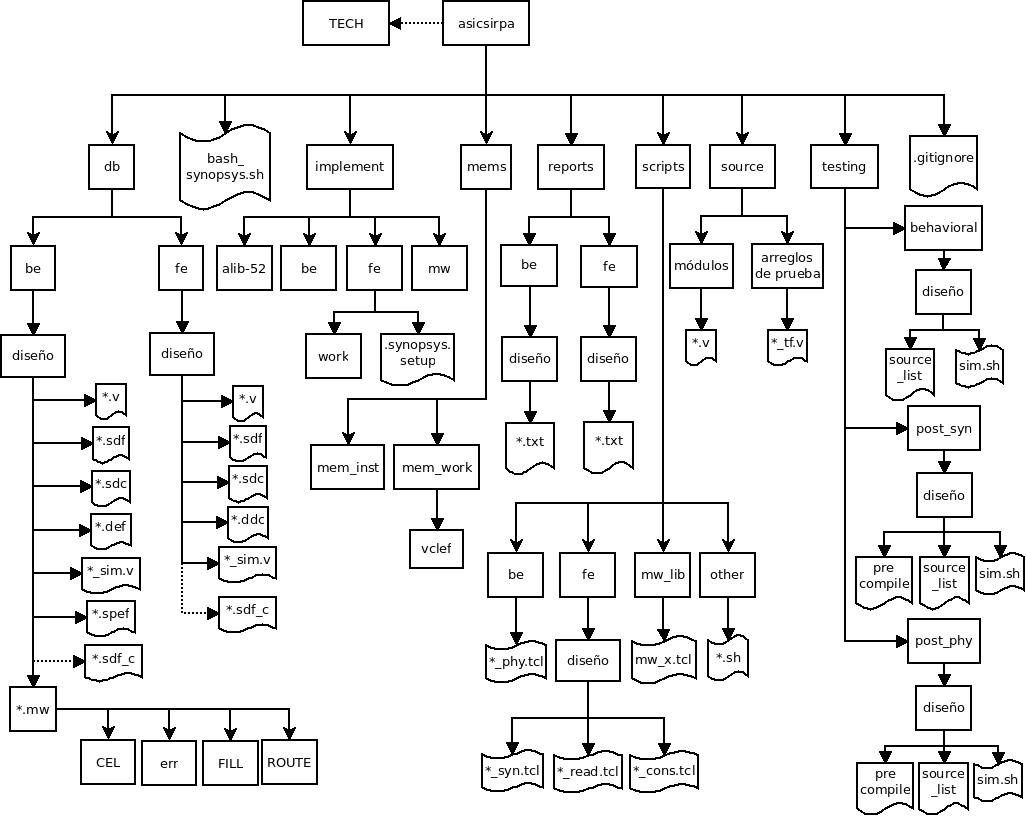
\includegraphics[width=\textwidth]{estructura.jpeg}
\centering
\caption{Esquema completo de la jerarquía de directorios y archivos que implementan el flujo de diseño digital. El bloque \textbf{TECH} hace referencia a la biblioteca de la tecnología, no es buena idea agregar este directorio en la misma ubicación que el proyecto ya que es un directorio de tamaño considerable y copiarlo en cada proyecto representa un mal gasto considerable de memoria, aunque los sistemas modernos tienen una gran capacidad de almacenamiento, siempre es más eficiente manejar únicamente un directorio para la tecnología.}
\label{directorios}
\end{figure}
Como puede apreciarse en la figura \ref{directorios} el directorio base del proyecto contiene hasta el momento siete directorios y dos archivos, uno de los cuales es oculto y carece de relevancia para el proyecto. Comenzando por el archivo \textbf{bash\_synopsys.sh}, tenemos un script de bash, que es una de las tantas consolas que ofrecen los ambientes linux, este script contiene punteros hacia los archivos ejecutables del juego de herramientas de Synopsys, la licencia para que puedan correr, y finalmente cualquier otro software a fín al proyecto pueda ser usado.

Dentro de la estructura propuesta existe un archivo que es importante para que el flujo de diseño sea más cómodo para el usuario, el archivo del que se habla es el archivo \textbf{.bashrc}, el cual es un archivo oculto y se ubica en el directorio principal del usuario, a este directorio suele denominarsele como: "HOME", es universal en cualquier computador con un sistema operativo linux moderno. Este archivo es ejecutado cada vez que se abre una terminal o consola de tipo bash, y le permite al usuario personalizar distintos aspectos de la consola, gracias a esta cualidad es posible abrir una terminal y contar con la posibilidad de disponer de las herramientas necesarias sin tener que ejecutar el script "bash\_synopsys.sh" cada vez que se abre una nueva terminal.

Este archivo (.bashrc) también permite crear variables con rutas relativas a directorios. El contexto en el que se establece la premisa de rutas relativas, corresponde a que el proyecto al ser de dimensiones considerables, involucra a varias personas, y entre otras cosas también existe una herramienta para el manejo de versiones "CVS" \cite{website:cvs}, además es probable que existan muchas copias del proyecto en distintos computadores o servidores.

Así, al hablar de rutas relativas se refiere a que cada computador tiene una ruta absoluta diferente hacia el directorio del proyecto, pero, una vez que se encuentre dentro del directorio del proyecto, las rutas hacia directorios y archivos se vuelven iguales para todos los involucrados. Mediante el uso de variables es posible usar un único comando de referencia en los scripts, y usando variables con rutas relativas, permite abstenerse de editar los scripts en cada computador. Más adelante se expondrá un poco más sobre la importancia de las rutas relativas cuando se hable de los scripts para ejecutar los procesos de síntesis. Podemos ver lo expuesto anteriormente en el diagrama de la figura \ref{bash_syn}.

\begin{figure}[h]
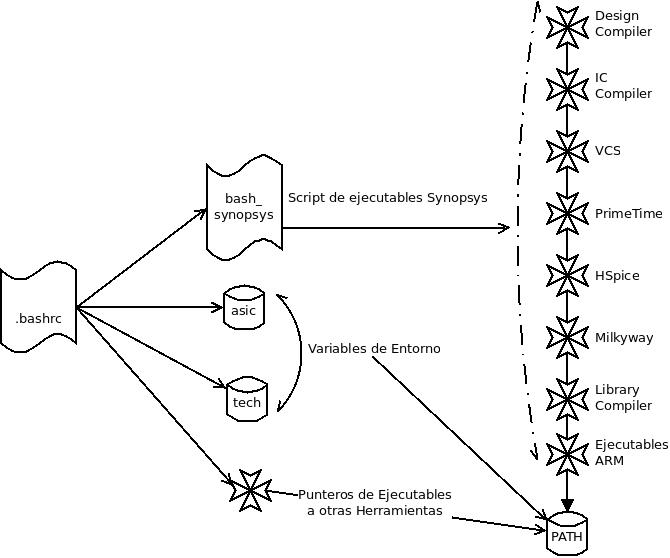
\includegraphics[width=\textwidth]{s_bash.jpeg}
\centering
\caption{Esquema ilustrativo de la relación entre los scripts de bash que inicializan las herramientas EDA y crean las varibles que contienen los punteros a los archivos y la biblioteca de la tecnología de integración}
\label{bash_syn}
\end{figure}

A continuación podemos observar un ejemplo que ilustra, la ejecución del script de bash para incluir en la variable de ambiente "PATH", las rutas a los ejecutables de las herramientas EDA (línea 8), y la creación de 2 variables con la ruta relativa al directorio base del proyecto (variable "asic", línea 3)


\definecolor{mygray}{rgb}{0.5,0.5,0.5}
\definecolor{mygreen}{rgb}{0,0.4,0.1}

\begin{lstlisting}[language=bash, numbers=left, keywordstyle=\color{blue}, commentstyle=\color{mygreen}]
# Home for working on the SiRPA ASIC Integration Project
asic=/home/rcastro/asicsirpa
export asic
# IBM technology files for the Integration Project (Library)
tech=/home/IBM/TECH
export tech
# Load the EDA Synopsys executables
. $asic/bash_synopsys.sh
# Load a text processor application
PATH=$PATH:/home/tools/sublime_text_3
export PATH
\end{lstlisting}


Retomando el diagrama de la figura \ref{directorios}, dentro del directorio del proyecto de integración encontramos siete directorios, de los cuales db, implement, reports y scripts presentan la misma estructura regular, pues en cada uno de estos directorios encontramos otros 2 directorios llamados be y fe, como podrá intuirse hacen referencia a "back end" y "front end" respectivamente, se decidió usar estas abreviaciones por su simplicidad ya que resumen muy concretamente a que hacen referencia y son muy intuitivas.

El directorio \textbf{db} es una abreviación a "Data Base", que en inglés significa base de datos, y precisamente es en este directorio donde se albergan las bases de datos y demás archivos que son producto de los procesos de síntesis, naturalmente en el subdirectorio fe sólo se almacenan los resultados de la sínteisis lógica de los módulos del proyecto.

El directorio \textbf{implement} alude al proceso de ejecución de las herramientas y los procesos de síntesis, este directorio no contiene archivos de gran relevancia para el proyecto, salvo el directorio \textbf{fe} el cual contiene el archivo oculto, \textbf{.synopsys\_dc.setup}, que es un script de \textit{TCL} con comandos de inicialización y preconfiguración de la herramienta \textit{Design Compiler}, este script es de vital importancia para que la herramienta opere de forma adecuada, más adelante se expondrá un poco más sobre este archivo. Este directorio se emplea para concentrar los archivos temporales que se producen cuando se trabaja con las herramientas de síntesis, los directorios \textbf{work} en fe, el cual contiene archivos que se generan al analizar el código fuente en \textit{HDL}, el directorio \textbf{alib-52} que contiene las bibliotecas producto de la compilación del diseño, esta biblioteca contiene información de caracterización de la biblioteca de la tecnología y sirve para acelerar compilaciones subsecuentes. Finalmente dentro del directorio \textbf{implement} tenemos otro directorio llamado \textbf{mw}, este directorio contiene los reportes y anotaciones de la ejecución de la herramienta \textit{Milkyway}, que es una herramienta de \textit{back end} y podría incluirse en el directorio \textbf{be}; sin embargo, se considera adecuado que esta herramienta tenga un directorio particular para sí, más adelante se explicará la funcionalidad de esta aplicación y el porqué de esta separación.

Siguiendo con los directorios que presentan regularidad, encontramos los directorios: \textbf{reports} y \textbf{scripts}, los cuales contienen reportes y scripts respectivamente. Los reportes generados son distintos de los que genera la herramienta a la hora de estar haciendo el proceso de síntesis, estos reportes corresponden a la información final de síntesis y proveen información útil en la toma de decisiones de las etapas posteriores. Luego los scripts, son los códigos principalmente en lenguaje \textit{TCL} donde se condensan los comandos que usan las herramientas para generar los procesos de síntesis. En el directorio scripts se observan otros dos directorios, \textbf{mw} y \textbf{other}, que contienen respectivamente contienen scripts para la herramienta \textit{Milkyway}, y de otras herramientas como por ejemplo \textit{MATLAB} y los generadores de memorias \textit{SRAM} de \textit{ARM}, los cuales serán expuestos más adelante.

Los tres directorios restantes, \textbf{mems}, \textbf{source}, y \textbf{testing}, no presentan una estructura regular como la que hemos visto hasta el momento, el directorio \textbf{testing} podría incluirse en esa categoría; sin embargo, la subdivisión que presenta es bastante puntual e intuitiva, así que se considera más práctica. Como se puede abstraer "testing", es una palabra en inglés cuya traducción es "pruebas", aquí se alojan los resultados de las distintas simulaciones con las que se valida la funcionalidad de los módulos sometidos al flujo, las simulaciones se subdividen en tres categorías, por comportamiento, en inglés, \textbf{behavioral}, post síntesis lógica (\textbf{post\_syn}), y post síntesis física (\textbf{post\_phy}). Estos tres directorios cuentan con 3 archivos principales, los punteros de compilación, archivos fuente, y un script en \textit{bash} que permiten invocar la herramienta de simulación y ejecutar las compilaciones y simulaciones respectivas, luego de la simulación puede que sea de interés guardar un vector de resultados en un archivo de texto. Así que los directorios de simulación presentan cuatro archivos importantes, los archivos extra que puedan encontrarse en estos directorios son producto de los apuntes y registros que genera la herramienta durante la compilación, y pueden ser obviados.

El directorio \textbf{source}, que se traduce como fuente, contiene dos categorías de directorios, el primero corresponde a los archivos \textit{HDL} con la información modular del diseño, es decir los archivos con la descripción por comportamiento del diseño, y también los archivos con los vectores de estimulos y arreglos o bancos de prueba, es decir los \textit{testbenchs o testfixtures}. Los primeros usados en el proceso de síntesis lógica, y los últimos necesarios para las simulaciones en los distintos dominios.

Por último tenemos el directorio \textbf{mems}, el cual es un directorio bastante particular. Contiene la información producida por los aceleradores de diseño de \textit{ARM}, los cuales generan celdas de memoria \textit{SRAM}. Se trata este proceso aparte ya que los programas para generar las celdas de memoria tienen una metodología de trabajo un poco diferente de la del flujo digital que se ha venido exponiendo. La justificación de manejar estos directorios aparte recae en no mezclar las metodologías de trabajo; sin embargo, el producto final de este procedimiento se integra a la estructura que se ha venido describiendo, es decir se generan bases de datos para las etapas de \textit {back y front end}, posteriormente se ahondará en detalles cuando se expongan los scripts de síntesis de las \textit{SRAM}.

En este directorio (\textbf{mems}), se encuentran dos directorios principales, \textbf{mem\_inst}, el cual contiene los ejecutables de las herramientas de \textit{ARM} para sintetizar las memorias, es importante que sólo exista una única copia de este directorio, ya que es muy pesado (en términos de espacio, cerca de 2 GB), y generaría saturación en un repositorio, que se debe mantener simple y con la menor densidad posible. El otro directorio es \textbf{mem\_work}, el cual contiene el resultado de la síntesis de las celdas \textit{SRAM} y finalmente \textbf{vclef} el cual es un archivo con la información de los metales y el enrutado de la celda \textbf{SRAM} física, este último se crea con el fin de facilitar la ejecución de la herramienta \textit{Milkyway} y generar las base de datos necesarias para los procesos de \textit{back end}. Nuevamente esto será discutido en detalle en un apartado posterior.



\section{Scripts de Front End}
\label{sec:syn_s}
\subsection{Script de síntesis lógica}
\label{script_syn}
En la figura \ref{s_syn} se observa como la síntesis lógica se ejecuta mediante tres scripts, dos de los cuales son auxiliares al script de síntesis, los scripts se nombran de acuerdo con un nombre representativo del diseño con el que se trabaja, aunque suele ser conveniente nombrar los archivos de la misma manera al módulo principal, si este nombre es muy largo, es preferible optar por un nombre representativo.

\begin{figure}[h]
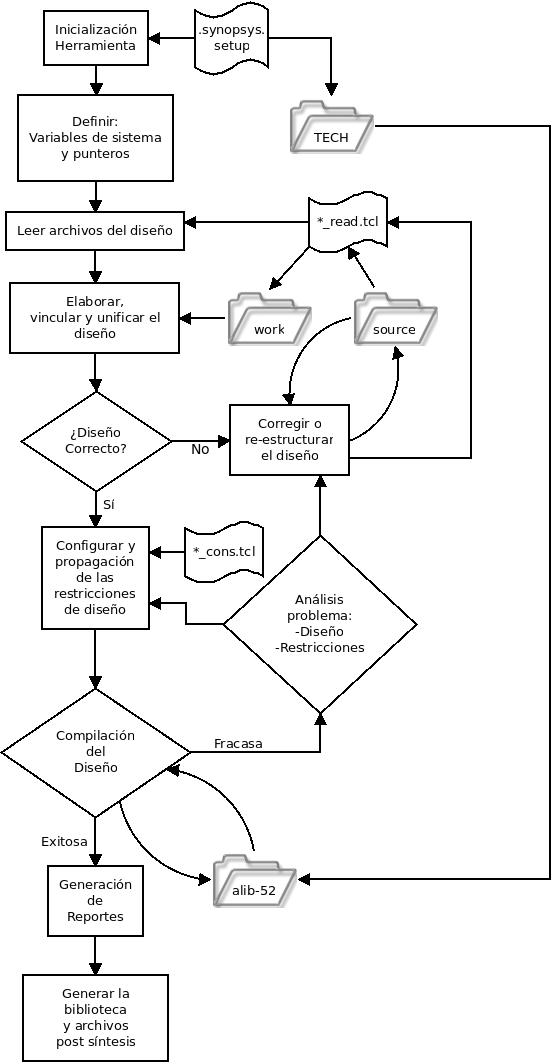
\includegraphics[scale=0.55]{log_syn.jpeg}
\centering
\caption{Diagrama de flujo del scripting que ejecuta la síntesis lógica}
\label{s_syn}
\end{figure}



Es aconsejable separar las instrucciones de síntesis de la herramienta para no generar scripts densos en código y modular las operaciones ejecutadas por la herramienta.

Existe un único flujo en la ejecución de los scripts. El script principal, (*\_syn.tcl) contempla el diagrama de la figura \ref{s_syn}, a partir de la etapa en la que se definen los punteros y las variables del sistema, continúa en línea recta hasta la generación de la base de datos y demás archivos post síntesis. En un apartado anterior se mencionó sobre la importancia del script \textbf{.synopsys\_dc.setup}, este archivo contiene comandos y procedimientos de \textit{TCL} que ejecutan tareas configuración, tal como inicialización de parámetros y variables, declaración de las bibliotecas de diseño.

Cuando la herramienta \textit{Design Compiler} es invocada, ésta busca el archivo configuración en la dirección desde dónde fue invocada, al leer los archivos la herramienta tendrá la información de la ruta hacia las bibliotecas, y cualquier otra personalización que el usuario considere necesaria para facilitar el uso de la herramienta, como crear un alias para comandos en particular, definir la ruta del directorio \textit{alib-52}, el cual se usa para sintetizar una biblioteca reducida y acelerar el proceso de compilación lógica, aunque este es un directorio que le facilita la operación a la herramienta, y las bibliotecas generadas pueden ser utilizadas en etapas posteriores del diseño, no es imperativo que este directorio permanezca en el proyecto, y tampoco es imperativo incluirlo en un repositorio, ya que versionarlo carece de sentido práctico.

Otro de los usos más significativos que se le da al archivo \textbf{.synopsys\_dc.setup} en este proyecto es adquirir variables del sistema operativo para definir variables locales al entorno de la herramienta, estas consisten consiste en rutas relativas al directorio base del proyecto y el directorio base de la biblioteca de la tecnología.

Crear este tipo de variables facilita que los scripts puedan parametrizarse y estos sean capaces de ser usados en distintos equipos sin tener que alterarlos o acondicionarlos significativamente, para que puedan ser funcionales independiente a las rutas locales de los archivos en otros equipos.

Cabe destacar que no toda la configuración de parámetros y variables se realiza en este archivo, y aunque es posible, tampoco es eficiente hacerlo. Este archivo tiene un caráter más genérico. Su función es poner la herramienta a punto para que este en capacidad de sintetizar correctamente cualquier diseño. Las particularidades de los diseños que se trabajan son contempladas en el script de restricciones (constraints), así que no todas las restricciones de diseño se incluyen en este script, sólo las que son universales para cualquier diseño. 

Una vez que la herramienta ha sido inicializada, se procede a configurar variables y parámetros propios del diseño con el que se trabaja. Estos son principalmente variables de rutas hacia el destino de los archivos de salida, y reportes, así como punteros hacia la ruta a bibliotecas auxiliares para el diseño en particular. Así también se crean variables con el nombre del proyecto para que al generar los archivos de salida se usen los comandos de forma paramétrica. Es decir los comandos dependen del valor o contenido de las varibles, esto último se realiza con la finalidad de tener un script genérico, al cual se le deba dar una edición mínima cuando deba ser adaptado a otro diseño.

\subsubsection{Script de lectura de archivos fuente}

Cuando finalmente se han definido todos los parámetros y variables generales para el diseño particular con el que se trabajará, se procede a leer los archivos fuente del diseño, esto corresponde a los módulos descritos en \textit{HDL}. El conjunto de estos archivos \textit{HDL} suelen denominarse como diseño descrito en \textbf{RTL}\footnote{RTL, refiere a Register Transfer Level. Su traducción corresponde a nivel de transferencia mediante registros, dentro del argot del diseño VLSI refiere a la metodología con la cual se describe un dispositivo digital usando un lenguaje de alto nivel, cuya semántica concuerda con el comportamiento del dispositivo digital.} La herramienta debe analizar cada archivo, dependiendo del proyecto pueden existir una enorme cantidad de módulos por analizar, esta es la razón por la que se genera un script de lectura de módulos.

Usando las ventajas de los lenguajes compilados como lo es \textit{TCL}, la lectura y análisis de los módulos se puede realizar de forma programática. En el script \textbf{*\_read.tcl} se usa una variable con el puntero hacia el directorio base de los archivos \textit{HDL} fuente, luego mediante una subrutina de \textit{TCL} se crea una colección con los directorios que contienen los distintos módulos posteriormente se ejecuta un pequeño algoritmo recursivo que recorre las colección de los directorios, para cada directorio se crea otra colección con los módulos, los cuales nuevamente son leídos de manera recursiva. Al recorrer esta última colección se ejecuta el comando de análisis de la herramienta, así se analizan todos los módulos del diseño de forma automática, sin tener la necesidad de incluir en el script la misma instrucción repetida para leer cada posible archivo del proyecto.

\begin{figure}[h]
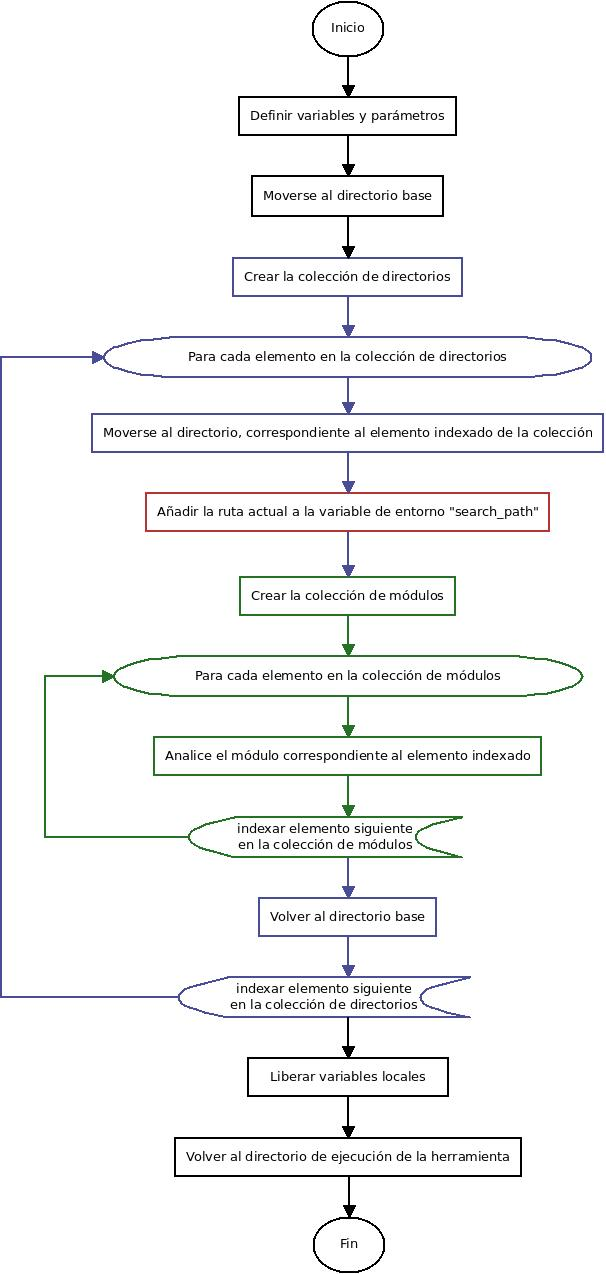
\includegraphics[scale=0.45]{read_script.jpeg}
\centering
\caption{Algoritmo recursivo de lectura y análisis de los módulos \textit{HDL} del diseño}
\label{s_read}
\end{figure}

En la figura \ref{s_read} se observa un diagrama de flujo, con el resumen gráfico del algoritmo descrito en los párrafos anteriores, cabe destacar que en el bloque que indica la definición de variables y parámetros hace referencia a variables locales para ejecutar las tareas de lectura, aunque en realidad únicamente se crean punteros (a los que también llamaremos variables de ruta) hacia las rutas base de los archivos fuente.

Cabe destacar que para algunos diseños, las variables de ruta no necesariamente apuntan a directorios con contenido \textit{HDL}, pues como suele hacerse en proyectos muy grandes, conviene dividir el diseño general en subdiseños más compactos, esto último implica que para algunos proyectos es preferible leer las bases de datos generadas para otros diseños, pues es más práctico.

Otra observación que se debe realizar al diagrama de la figura \ref{s_read} es que no en todos los diseños es necesario crear una colección de directorios, pues si todos los archivos fuente de ese diseño se concentran en un directorio, recorrer la colección de directorios carece de sentido. Consecuentemente puede omitirse el lazo de color púrpura, correspondiente al algoritmo iterativo de indexación de directorios. El único lazo estrictamente necesario para leer los archivos fuente, es el lazo en color verde. Se incluyen ambos lazos en la figura \ref{s_read}, y se expuso el proceso de lectura y análisis con los dos lazos para ilustrar el caso más general de lectura de archivos fuente. Naturalmente los scripts deben ajustarse a la estructura particular del diseño; sin embargo, el algoritmo expuesto es fácilmente adaptable a cada caso.

Siguiendo con la figura \ref{s_read}, y dándole continuidad a la idea expuesta en el párrafo anterior,procede declarar que conviene conservar el bloque de añadir en la variable "search\_path" la ruta actual (bloque en color rojo), ya que al usar el comando de análisis de la herramienta \textit{Design Compiler}, si la ruta relativa al archivo no se ha incluído a la variable de búsqueda (search\_path) la herramienta ofrecerá un error, pues se pretende acceder a una ubicación que no ha sido autorizada para la herramienta.

La variable "search\_path", es una variable propia del entorno de las herramientas de \textit{Synopsys}, su función es manejar una colección de ubicaciones o rutas permitidas para que le herramienta pueda leer y escribir archivos.

Finalmente conviene volver a la ubicación desde donde se ejecutó la herramienta para evitar crear archivos de apuntes, o archivos temporales con poca relevancia para el proyecto, en directorios ajenos a los destinados para esta tarea. Basta decir que liberar todas las variables locales al finalizar una subrutina es una buena práctica de programación, así que es conveniente hacerlo.

Volviendo a la ejecución del script principal de síntesis, cuando ya todos lo módulos son leídos, en el directorio work se crean archivos con información sobre el resultado del análisis de los módulos, de momento estos archivos serán fundamentales para avanzar en el flujo de síntesis, pero una vez acabado el flujo y habiendo generado la base de datos del diseño, no son tan relevantes.


Dicho lo anterior, se debe proceder a elaborar el diseño, esto consiste en definirle a la herramienta cuál es el módulo principal del diseño, posteriormente se deben vincular y unificar todos los módulos. La vinculación y unificación establece la jerarquía modular del diseño y resuelve la interdependencia de los módulos.

En la figura \ref{s_syn} se observa un bloque condicional (diamante de decisión), evaluando la condición si el diseño es correcto. En otras palabras, la herramienta evalúa entre otras cosas, si la semántica del código es correcta, no existen errores sintácticos y todas las dependencias se cumplen. Este bloque condicional no se asocia a una subrutina programática en el script, de hecho ninguno de los bloques condicionales que se aprecian en este diagrama lo hace, en la semántica del flujo también interviene el criterio del diseñador y este es un claro ejemplo de esta situación.

Muy probablemente cuando se le solicite a la herramienta evaluar el diseño, aparecerán mensajes de información, alarmas, y en el peor de los casos, errores. El diseñador entonces, deberá evaluar el escenario con el que se enfrenta, corregir los errores es imperativo; sin embargo, muchos de las alertas son tolerables o inofensivas, así que de acuerdo con la experiencia del diseñador se deberá mejorar o no el diseño, y solucionar o aprobar los mensajes de alerta. ¡Un ingeniero en diseño VLSI, debe aprender a vivir bajo el warning!


Si el diseñador no se siente satisfecho con el resultado de la comprobación de la herramienta, y los mensajes sugieren que debe hacer correcciones a los archivos fuente del diseño, lo más sensato es ponerse en contacto con el departamento o personal encargado del diseño por comportamiento y exponer la situación. En algunos casos el diseñador de \textit{front end} podrá verse arrastrado a analizar y corregir el código fuente, esto suele ser muy raro, ya que las tareas en el flujo de integración suelen estar muy bien definidas de acuerdo con departamentos creados para delimitar y definir tareas y responsabilidades, al menos es así en las industrias de gran envergadura; sin embargo, para diseños de baja envergadura, e instituciones académicas es común encontrar a una única persona realizando todas las tareas relacionadas al flujo.

Cuando la comprobación del diseño es aprobada, lo siguiente es establecer las cotas del comportamiento o dicho de otro modo, las restricciones de operación del diseño y propagarlas por la jerarquía, así todas las dependencias tendrán las mismas condiciones de funcionamiento . Esto quiere decir que se deben definir las condiciones bajo las que el diseño va a operar, como por ejemplo, se definen las características de señales críticas y de alta importancia para el diseño como el reloj.

\subsubsection{Script de restricciones}

En esta etapa es donde se invoca el script de restricciones, en inglés "constraints". Este script se encuentra en el flujo del diagrama de la figura \ref{s_syn} como \textit{*\_cons.tcl}. Para este script no hace falta mostrar un diagrama de flujo sobre su comportamiento ya que en principio sólo define parámetros y variables de entorno de la herramienta \textit{Design Compiler}.

A continuación se presenta un pequeño resumen de los parámetros que se consideran suficientes para cumplir a cabalidad las expectativas de desempeño del diseño.

\begin{itemize}
\item \textbf{Señal de reloj:} {Esta señal necesita en principio ser creada, con esto se refiere a generar un objeto\footnote{Entendiendo por objeto al concepto de programación de alto nivel asociado al ente programático capaz de presentar una colección de atributos y permitirle a funciones complejas invocarle y utilizar sus atributos en tareas específicas. Para más información se invita al lector a que consulte un diccionario sobre terminología en el diseño de software} para que la herramienta pueda crear un árbol de reloj hacia los módulos sincrónicos del diseño. Debe definirse un nombre representativo para la señal en el diseño, hay que recalcar que es conveniente definir una nomenclatura estándar para un proyecto grande que involucre diseños jerarquizados, así cada subdiseño tendrá una señal de reloj con las mismas propiedades y un mismo nombre.

Una vez se crea el objeto "señal de reloj", se definen sus propiedades, en esencia, se define el periodo, la incertidumbre, el sesgo y la latencia de la señal, siempre asociando cada propiedad al objeto "señal de reloj" que ha sido creado. Pueden definirse más propiedades, o las mismas de una forma diferente, ya que la herramienta lo permite, pero se considera que estas son suficientes.}

\item \textbf{Propagación de señales:} {Cuando se tienen señales universales a todos los módulos secuenciales, como lo suelen ser las señales de reloj, reset (reinicio), enable (habilitación), preset (preconfiguración), etc. Es posible y es conveniente definir condiciones de comportamiento para la herramienta, ya que esta suele hacer cosas indeseables como colocar buffers en el camino de propagación de señales críticas. Una compuerta lógica, como lo es un buffer presentará efectos de retardo de propagación, lo cual a posteriori se traduce en problemas de sincronización. Es por ello que para estas señales se define un atributo para que la herramienta no realice optimizaciones en ellas. Y el diseñador tendrá un mejor control sobre lo que suceda con esas señales. En este caso únicamente la señal de reloj y reset se definen como intocables.}

\item \textbf{Comportamiento de otras señales:} {Para generar de forma adecuada los modelos simulación, y hacer estimaciones certeras sobre la sincronización de las señales, es beneficioso definir los retardos de propagación de entrada y salida de todas las señales, excepto las mencionadas anteriormente (reloj y reset). Los estímulos en el cableado no se propagan de forma inmediata, por lo que se debe procurar emular un comportamiento cercano a la realidad, para que el resultado de la síntesis del diseño sea lo más confiable posible.}

\item \textbf{Modelo de carga para el cableado:} {Continuando con la idea de generar un modelo lo más realista posible, se deben considerar las características energéticas del cableado.

Conocer las parasitancias de los materiales que se pretenden usar para alimentar e interconectar los módulos del diseño, permite elaborar modelos de comportamiento más cercanos a la realidad. Conocer las propiedades resistivas ayuda a elaborar estimaciones de consumo y desempeño energético, los efectos capacitivos e inductivos permiten evaluar los fenómenos de retardo en las señales, consumo de potencia dinámica, cuando hay conmutación en las señales. Incluso, es posible considerar interferencia por radiación de campos eléctricos y en menor medida los magnéticos. Conocer el área que el enrutado ocupará también es importante para que la herramienta genere una buena optimización del colocado y el enrutamiento. El modelo de cableado o alambrado, es fundamental en sistemas de integración modernos, donde la escala de integración es cada vez más pequeña, a partir de los 300 nm es imperativo contemplar estos efectos.}

\item \textbf{Celdas de conducción:} {El nombre de este atributo, es "driving\_cell", la traducción literal al español no es muy certera; sin embargo, es suficientemente clara. La herramienta necesita que este atributo sea definido para usar una celda adecuada, un buffer, para conectar los módulos del diseño a los puertos de entrada y salida. Esto debe hacerse, en las señales que se propagan hacia puertos de entrada y salida principales e intermodulares.

Una carga excesiva para las señales, suele asociarse a pérdida de información, e inclusive inoperabilidad de algunos segmentos, no se entrará en detalles sobre porqué es importante respetar los fanouts\footnote{El fanout o abanico de salida hace referencia a la máxima cantidad de carga (conexiones) que una señal o puerto es capaz de manejar, hasta que por razones de potencia, esta se empiece a degradar y la señal alcanza niveles de tensión que pueden conducir a la metaestabilidad.} de las señales.

Contemplar las capacidades de conexión de una señal hacia múltiples dependencias, y garantizar la integridad de la información transmitida por dicha señal, es una práctica muy favorable para garantizar la operación exitosa de un diseño. Es por ello que en este apartado también se define un valor máximo de fanout}

\item \textbf{Factor de Actividad:} {El factor de actividad es un parámetro que le indica a la herramienta, como promediar el consumo de potencia dinámico de las señales. En la literatura este parámetro se denomina con la letra griega alfa (\textbf{$\alpha$}).

El factor de actividad, $\alpha$, indica cuantas veces conmuta una señal por ciclo de reloj, naturalmente en un diseño complejo habrán muchas señales con factores de actividad diversos y este cambiará de acuerdo con la tarea que se ejecuta. El valor adecuado a usar en este parámetro responde más a la evidencia empírica y a la experiencia del diseñador.\cite{book:weste2005}

El uso de este parámetro ofrece la posibilidad de generar un reporte de estimación de consumo energético más cercano al comportamiento real del diseño.}
\end{itemize}

Existen muchos otros parámetros que permiten personalizar y condicionar de forma más profunda el diseño, no obstante se expusieron las principales categorías que se deben contemplar y algunas particularidades que se consideran importantes para generar modelos suficientemente cercanos a la realidad. La selección de parámetros suele ser hecha por los ingenieros que se definen los alcances y el desempeño esperado del diseño.

Una vez que las restricciones de diseño han sido definidas y propagadas. Se procede a compilar el diseño, que es la esencia de la síntesis lógica. La compilación le indica a la herramienta que debe generar un nuevo proyecto usando las celdas estándar de la biblioteca de la tecnología, e implementar la estructura abstraída del modelo por comportamiento analizado. En resumen a partir del resultado del análisis del diseño en \textit{HDL} se crea una nueva estructura que mantiene la jerarquía de las funciones y tareas, pero estas ya no se implementan mediante código \textit{HDL} si no mediante elementos de circuitos digitales. En la figura \ref{comp} se observa una analogía gráfica de lo expuesto anteriormente.

\begin{figure}[h]
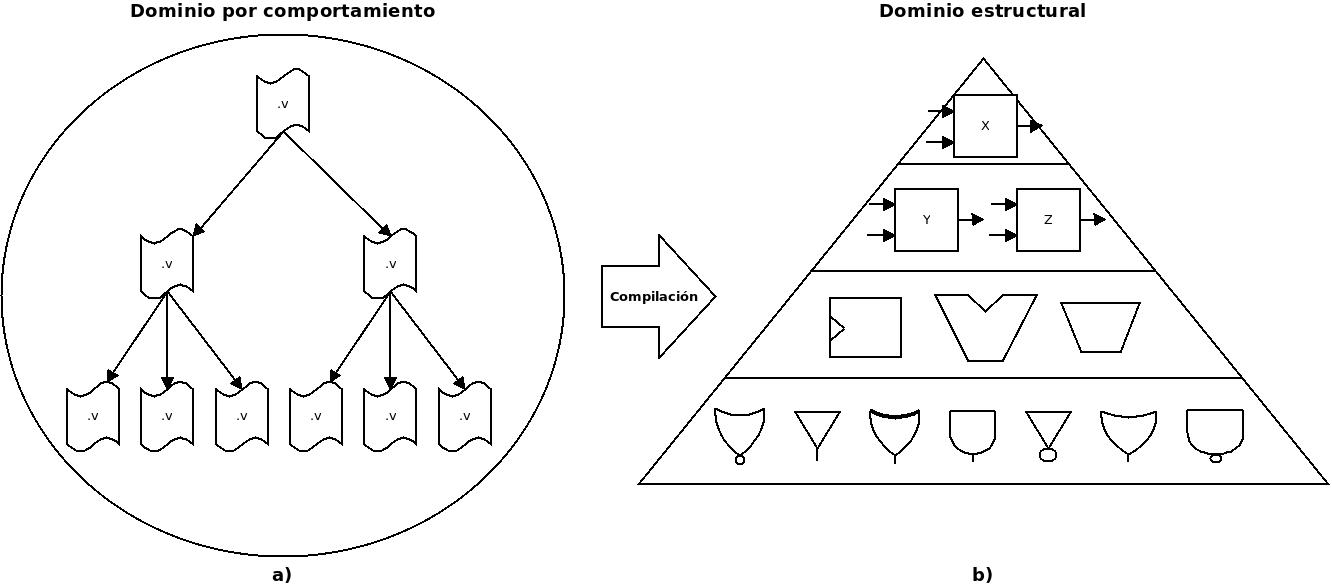
\includegraphics[width=\textwidth]{Compile.jpeg}
\centering
\caption{Ilustración del proceso de compilación. En figura \textbf{$a)$} se aprecia la estructura jerárquica de códigos en \textit{HDL}, y en la figura \textbf{$b)$} la jerarquía abstraída, implementada mediante distintos niveles de elementos digitales, pasando desde funciones complejas, módulos digitales avanzados, hasta compuertas lógicas fundamentales.}
\label{comp}
\end{figure}

Retomando la figura \ref{s_syn} recordamos que el bloque de compilación nuevamente es representado por un diamante de decisión, este diamante no refiere a un evento programático, si no a una etapa en la que el diseñador deberá evaluar si la compilación del diseño es satisfactoria. En esencia la compilación se corrobora mediante la solicitud de reportes a la herramienta, en este punto las bibliotecas compiladas en el directorio \textit{alib-52} y los alias creados en el script de inicialización son bastante útiles, ya que es posible repetir el procedimiento de compilación con relativa facilidad y rapidez.

Es conveniente desviar los resultados de la síntesis (compilación) hacia archivos, para mantener un registro. Esto permite llevar un registro del comportamiento de los diseños, y en caso de que se deba se podrá consultar el resultado de un proyecto anterior, para así evaluar si de ser necesario incluirlo en otro proyecto, ese proyecto anterior cumple las expectativas para el nuevo diseño.

La herramienta permite generar reportes de:

\begin{itemize}
\item \textbf{Sincronización (timing):} {Consiste principalmente en la tabulación de la información asociada a la propagación de la señal de reloj del circuito. Es un análisis que estima el retardo en el diseño basándose únicamente en la topología de las rutas de propagación de la señal de reloj.

A lo anterior se le conoce como \textbf{esfuerzo lógico}, por lo tanto la solicitud de este reporte a la herramienta, consigue un analisis de esfuerzo lógico en el diseño. La herramienta genera entonces un presupuesto teórico de cuanto debe tomarle a la señal, el propagarse a través de una determinada ruta, y evaluar, junto con la información suministrada por las restricciones del diseñador, y la información que aporta la biblioteca de la tecnología, si los datos llegan en el tiempo presupuestado, conocido como "slack MET"\footnote{Es posible ahondar más sobre qué es el "slack" y cual es su relevancia; sin embargo, este informe pretende desvelar el flujo de diseño digital. Se parte de la premisa que el lector comprende el uso de términos como: slack, hold time o setup time, hablar más al respecto está fuera del objetivo de este informe.}.}

\item \textbf{Potencia:} {Se refiere a una descripción resumida de las características de alimentación del diseño, esto se refiere a la tensión nominal de operación general de los dispositivos, el comportamiento estático y dinámico de las celdas estándar en términos de disipación energética. La información aparece resumida y tabulada, de forma que se puede encontrar cuanta energía se disipa o consume en un bloque en particular, entiéndase por bloque, los dispositivos combinacionales, secuenciales, señales, etc. }

\item \textbf{Área:} {Este reporte es un pequeño resumen del volumen o cantidad de celdas usadas (combinacionales y sequenciales), celdas extra como buffers, señales y puertos. Se hace una recopilación de el espacio que se preveé será necesario para colocar estos elementos en el espacio del dado de silicio, en etapas posteriores. La información más útil es que permite tener una idea del área necesaria para la colocación cuando deba diseñarse el floorplan, y le permite al diseñador efectuar un buen ansatz\footnote{Anzats: término de origen alemán, usado comúnmente por físicos y matemáticos para referirse a una estimación que permite resolver una ecuación o un problema. Refiérase a un diccionario de alemán.} al definir el tamaño del plano de colocación y enrutado (floorplan) del diseño durante la implementación física.}

\item \textbf{Celdas:} {Consiste en un listado de las celdas estándar necesarias para implementar el diseño. Se presenta en forma tabular, describiendo el nombre de referencia de la celda, el bloque de diseño donde es usada, el área que ocupa, y en que biblioteca donde se encuentra. Es útil para generar bibliotecas reducidas que permiten compilaciones más rápidas, y le permite al diseñador saber cuales bibliotecas debe tener en cuenta al hacer la implementación física o deba hacer simulaciones.}


\item \textbf{QOR (Quality of Results):} {Se traduce como calidad de resultados y es un compendio de varios de los atributos que se exponen en los otros reportes, tiene información sobre el área, la naturaleza de las celdas usadas, los caminos críticos de retardo, así como violaciones de sincronización, violaciones de reglas de diseño, inclusive presenta estadísticas del desempeño del computador que corrió la herramienta de síntesis. Se puede afirmar que es un resumen muy general del trabajo hecho en la síntesis del diseño.}
\end{itemize}

Finalmente es necesario guardar el proyecto y generar archivos que permitan evaluar si el proyecto cumple las expectativas de comportamiento, (ejecuta las funciones para las que fue concebido), y generar los archivos que permiten continuar el flujo de diseño. En resumen de lo anterior, se deben generar los archivos que tienen la información del resultado del proceso que se acaba de realizar, además generar los modelos para evaluar si los resultados siguen cumpliendo las expectativas de funcionamiento establecidas.

Los principales archivos generados son los siguientes:

\begin{itemize}
\item \textbf{DDC:} {Este es un archivo jerárquico, el cual define la estructura del diseño, qué celdas son necesarias para implementarla, todas las dependencias entre éstas, además de información de conectividad para implementar el comportamiento abstraído del diseño \textit{HDL}. Este archivo funciona como una base de datos que contiene toda la información expuesta en los reportes.

Este archivo es el estándar almacenamiento de la información post síntesis lógica de la herramienta \textit{Design Compiler}, es usado si en un futuro se necesita volver al diseño, usando el modo topográfico de la herramienta ya sea para editarlo y efectuar optimizaciones o recuperar información, como puede ser generar un reporte, etc. A partir de este archivo se puede continuar con la implementación física.}

\item \textbf{HDL:} {Este código HDL, que para fines prácticos en este informe consiste en códigos \textit{verilog}, se generá es considerablemente diferente del usado anteriormente, pues para la etapa de analisis del proyecto partíamos de un código fuente que describía el comportamiento del diseño, mediante un lenguaje de alto nivel. \textit{Verilog} ofrece la posibilidad de usar funciones de alto nivel para emular el comportamiento de los dispositivos digitales.

\textit{Verilog} también ofrece la posibilidad de implementar circuitos digitales mediante primitivas. Esto se refiere a que puede usar referencias a componentes digitales e interconectarlos de acuerdo con la semántica abstraída del código por comportamiento. A esta forma de codificación se le conoce como \textbf{GLD}\footnote{GLD, o GL refiere a Gate Level Description, en español, Descripción a Nivel de Compuertas. Este concepto refiere a una metodología de descripción de circuitos digitales, que permite establecer la relación entre componentes digitales, y enlazarlos de manera en que se forma una función o circuito más complejo.}

Es conveniente generar 2 archivos con la información del \textit{GLD}, esto con el fin de tener un archivo, que podrá ser usado por la siguiente etapa para iniciar la implementación física, y otro archivo para realizar la simulación post síntesis. La separación se debe a que el archivo que se use para la simulación necesita de una directiva adicional para leer el archivo que provee la información de los retardos, la presencia de esta directiva entra en conflicto con las herramientas de \textit{back end}, de esto se hablará más adelante. Sobra decir que conviene distinguir con un nombre adecuado ambos archivos, en este proyecto se usa la nomenclatura \textit{*\_syn\_sim.v} para diferenciar al archivo de simulación.}

\item \textbf{SDF:} {Standar Delay Format, en español, formato estándar de retardos. Consiste en un archivo, con información transferida por el ambiente de síntesis, con el fin de que otras herramientas de colocado y enrutado o simuladores, puedan usar la información de restricciones y retardos. En el caso de la simulación se obtienen resultados más cercanos a la realidad y este archivo permite una guía para que las herramientas de colocado y enrutado puedan optimizar el área en función de las restricciones de tiempo de las señales.}

\item \textbf{SDC:} {Synopsys Design Constraints, cuya traducción corresponde a Restricciones de Diseño de Synopsys. Consiste en un compendio de las configuraciones de los retardos que definen el comportamiento de los puertos y algunas señales, pricipalmente se configura el comportamiento de los retardos de los vectores de entrada y salida del diseño, y de como intervienen los buffers asociados a estos puertos. Se definen, el modelos de cableado y las unidades generales del diseño.}

\end{itemize}

Es posible exportar algunos archivos adicionales; sin embargo, los archivos anteriormente descritos son los necesarios y son suficientes para avanzar en el flujo.

\subsection{Simulación Lógica: evaluación pre y post síntesis lógica}
\label{sec:log_sim}
Los reportes generados permiten evaluar la calidad de la síntesis efectuada; sin embargo, para garantizar que el diseño funciona de manera adecuada, es necesario efectuar una verificación funcional. La verificación consiste en estimular el diseño de la misma manera que el modelo \textit{RTL}, o modelo por comportamiento.

En el directorio testing de la figura \ref{directorios} se encuentran 3 directorios, dos de los cuales se asocian al proceso de \textit{front end}, y corresponden a los directorios \textbf{behavioral} y \textbf{post\_syn}. Todos los directorios contenidos en el directorio de testing tienen la misma estructura y archivos muy similares.

Los directorios de simulación contienen, un script de precompilación y o simulación, uno ó dos archivos sin extensión que funcionan como punteros al invocar la herramienta de simulación. La función de los archivos sin extensión es indicarle a la herramienta donde se encuentran los archivos necesarios para correr una simulación.

En el caso de una simulación por comportamiento (\textit{behavioral}) únicamente se necesitan, los archivos \textit{RTL} del diseño, y el archivo de estimulo (banco o arreglo de pruebas), estos son indexados con el archivo sin extensión denominado \textbf{source\_list}. Entonces al ejecutar el script de simulación, se corre el comando de \textit{bash} para invocar la herramienta. Este proceso se ilustra en la figura \ref{beha_sim}

\begin{figure}[h]
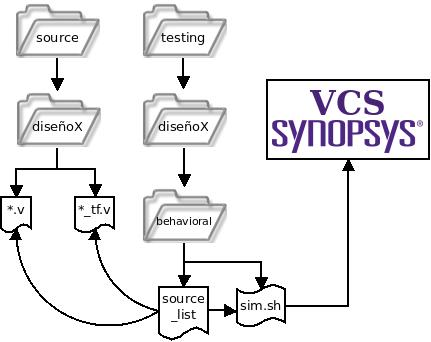
\includegraphics[scale=0.7]{beha_sim.jpeg}
\centering
\caption{Estructura del script de simulación por comportamiento. El archivo \textit{source\_list} apunta hacia el RTL, que se ubican en algún subdirectorio de \textit{source}. El script de simulación llama al archivo \textit{source\_list} al invocar al simulador \textit{VCS}}
\label{beha_sim}
\end{figure}

Para la simulación post síntesis se tiene una estructura similar, pero se tienen dos archivos sin extensión, el primero es el archivo que le indica a la herramienta cuales son los archivos necesarios para la precompilación, estos corresponden al archivo de la tecnología que contiene la biblioteca de simulación, el archivo \textit{HDL} con el netlist generado en la síntesis lógica, para efectos de este proyecto archivos \textit{*\_syn\_sim.v}, y dentro de este último debe estar la directiva de anotación de los retardos para ese diseño indicando la ruta del archivo \textit{*.sdf}. Esta directiva puede incluirse de forma manual, editando el archivo del netlist con algún procesador de texto, o se puede hacer de forma programática utilizando comandos de \textit{TCL} en el script de síntesis, naturalmente es más eficiente usar el segundo método.

La simulación post síntesis requiere que el simulador genere un objeto de alto nivel con las celdas estándar, y el comportamiento del retardo de las señales, es por ello que debe ejecutarse la precompilación y la lectura del archivo \textit{*.sdf} con el fin de que en la simulación pueda contemplarse el efecto de los retardos de propagación de las señales. Se genera un nuevo archivo con los retardos \textbf{*.sdf\_c} y este es el que será usado por el simulador. En la figura

\begin{figure}[h]
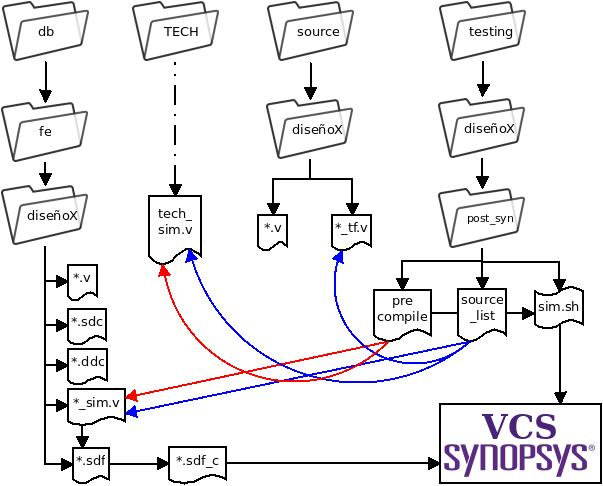
\includegraphics[scale=0.7]{post_syn_sim.jpeg}
\centering
\caption{Estructura del script de simulación post síntesis. El archivo \textit{precompile}, apunta a la biblioteca de simulación y al netlist, eñ \textit{source\_list} apunta hacia el netlist, el código de estímulo, y la biblioteca de simulación. El script de bash, invoca a la herramienta de simulación, realizando primero la precompilación y luego llama al archivo \textit{source\_list} para realizar la simulación}
\label{psyn_sim}
\end{figure}

\section{Scripts de Back End}
\label{sec:phy_s}
\subsection{Script de implementación o síntesis física}
Las herramientas de \textit{Synopsys} siguen un patrón similar en la ejecución de los flujos de síntesis. Nuevamente, conviene tener variables relativas hacia los directorios clave para que la implementación pueda ser ejecutada sin importar la ruta absoluta hacia los directorios. Además se deben definir las variables nativas de la herramienta que garantizan que el flujo será exitoso, tal como los punteros e identificadores hacia las bibliotecas.

Es posible iniciar la implementación de diversas maneras, en el caso del flujo propuesto en este trabajo comienza definiendo las variables principales para la celda física. En el entorno físico de \textit{Synopsys}, la base de datos que contienen la información de la celda, o las celdas físicas se llaman \textit{Milkyway}.

Antes de abrir o crear una base de datos o biblioteca \textit{Milkyway} se deben definir ciertos parámetros y aportarle a la herramienta información importante para la implementación. Esta información corresponde principalmente al nombre de las redes de alimentación y los coeficientes de tiempo de la tecnología, al hablar de coeficientes de tiempo, se refiere a los retardos por efectos parasíticos, que en esencia son los efectos capacitivos y resistivos de los puertos de los transistores \textbf{(Coeficientes RC)} y por lo tanto los \textbf{taus}\footnote{Recordar que "Tau" ($\tau$) corresponde a la constante de carga de una red capacitiva en un circuito eléctrico} de los puertos entrada y salida de cada celda estándar en la tecnología.

Los archivos que contienen la información de los coeficientes se llaman \textit{TLUPlus}, su formato consiste en una base de datos binarios tabulados. Esta información es fundamental en la extracción de los efectos de retardo debido a las parasitancias propias de la tecnología \textit{CMOS}. Si estos no son especificados no se podrá habilitar la "extracción RC" y tener estimaciones de retardo, y consumo dinámico más precisas que serán necesarias para un analisis más exhaustivo con las herramientas \textbf{Primetime} y \textbf{HSpice}.

Una vez se hayan definido los archivos \textit{TLUPlus} y demás parámetros para la celda \textit{Milkyway}, se puede abrir o crear la biblioteca. En este punto es posible tomar diversos caminos para resolver un diseño. Idealmente es posible generar un único diseño jerárquico donde existe una única base de datos, y los subdiseños pueden ser implementados como celdas dentro de la base de datos general del proyecto, así se puede y resolviendo el diseño desde una estrategia que en la jerga del diseño de software se conoce como \textbf{"BottomUp"}. 

Existe otra posibilidad en la que se pueden generar bibliotecas \textit{Milkyway} para cada subdiseño del proyecto principal y al final se exporta una celda con la información del diseño y se usa como una nueva celda estándar, en un diseño futuro (archivo de extensión \textbf{DEF}); sin embargo, aún no ha sido posible determinar la metodología exacta con la que \textit{IC-Compiler} realiza el manejo de los \textit{"Hard-Macros"}.

Es probable que no sea posible terminar un diseño en un único intento, es por ello que el script que se muestra, tiene una bloque condicional el cual se encarga de buscar el archivo \textit{Milkyway} que contiene la información de la celda o el diseño que interesa trabajar. Este condicional evalúa si la base de datos (.mw) existe. Con esa premisa se toma la decisión de abrir la base de datos o en su defecto crearla.

En el caso de que la base de datos exista y se deba abrir alguna celda en particular, conviene dejar el script principal o de inicialización del diseño hasta aquí. A partir de este punto el diseñador tiene múltiples caminos para decidir que hacer con su diseño y no hay una única ruta posible. En este punto es posible invocar múltiples para realizar tareas como evaluación de reglas DRC, análisis de sincronía de señales, re-enrutado selectivo, re-estructuración del colocado de las celdas, optimización de enrutado de acuerdo con criterios de área, potencia, o sincronía, entre muchas otras opciones.

Siguiendo el flujo del diagrama, y asumiendo que se trabaja con un proyecto nuevo, lo que procede es ejecutar el script que importa el diseño. Hay 2 formas principales para cargar un diseño, leyendo un archivo "GL" (HDL a nivel de compuertas) o leyendo un archivo ".ddc", ambos le indican a la herramienta que mediante la base de datos de las celdas estándar de la tecnología se importen las celdas físicas necesarias para iniciar el layout.

La importación del diseño suele involucrar los siguientes procesos: lectura del archivo fuente, la vinculación que resuelve las referencias del diseño y establece la jerarquía de los módulos, luego se desencadena el proceso de remover las celdas multiplicativas instanciadas de la biblioteca jerárquica, esto significa que se genera un nuevo bloque jerárquico que abstrae todas las jerarquías de las instancias y las unifica en una celda. Por su puesto todos estos pasos pueden hacerse por separado, pero la herramienta al importar un diseño los hace de forma automática.

\subsubsection{Floorplan}

Luego de invocar las celdas físicas, la herramienta provee una nueva ventana para visualizar la evolución del layout del diseño. Se procede a definir el floorplan (plano del circuito), esto corresponde a las dimensiones del dado (die o dice). Existen varias formas para establecer un floorplan, que siempre será un rectángulo ya que es la geometría que permite maximizar el aprovechamiento del área al usar celdas con formas de cuadriláteros.

Valiéndose del reporte de área generado en la síntesis lógica y mediante un par de ecuaciones cuadráticas simples, es posible extrapolar las dimensiones del floorplan, habrá que considerar que tan simétrico conviene hacer el espacio o si otra relación de tamaño permite una mejor distribución de las celdas y un diseño más compacto. El diseñador deberá contemplar un presupuesto extra en las dimensiones para el enrutado general, y garantizar un espaciado suficiente para evitar problemas de congestión y demás "DRCs". Además se debe contemplar un margen para puertos de entrada/salida (I/O) y los anillos de alimentación de los cuales se hablará más adelante.

Generar el floorplan de forma manual, y de una forma correcta responde más a la experiencia y la habilidad del diseñador para realizar un buen \textit{ansatz}. Típicamente se deben hacer unas cuantas iteraciones para encontrar el mejor tamaño y relación de aspecto del floorplan. La herramienta permite usar otras metodología para establecer el floorplan, la forma más cómoda que ofrece la herramienta es proveer la relación de aspecto, los margenes desde los puertos I/O hacia el área de colocado, y finalmente el porcentaje del área utilizable para el colocamiento de las celdas, entre más bajo sea este valor, menos probable será enfrentar problemas de congestión y por lo tanto más fácil conseguir un enrutado completo y funcional, pero esto implica que se desaprovecha un porcentaje considerable de área.

Una vez que se haya definido el floorplan se procede a colocar la celdas y a legalizar el colocado, que corresponde a que la herramienta 
efectúe un analisis de posibles conflictos debido a la ubicación de las celdas, así se reubican las celdas estándar del diseño, para evitar cualquier conflicto que se pueda encontrar debido a la colocación de las celdas.

Como ya se mencionó, si se establece un diseño jerárquico, y ya se ha logrado conseguir la síntesis física de los subdiseños que componen el proyecto actual, es posible cargar la información de estas macroceldas ya generadas y tenerlas como premisa para el colocado y enrutado de la nueva macrocelda, esto se logra al crear \textbf{plan\_groups}.

Los "plan\_groups" son áreas restringidas para que las celdas asociadas a una macrocelda se coloquen en una región específica, la colocación de las celdas se hacen a groso modo. Si existen celdas o diseños ya implementados la herramienta puede abstraer el colocamiento que se definió previamente para ese subdiseño y usarlo como punto de partida para agilizar el colocamiento del nuevo diseño, suele complementarse con la lectura de archivos de restricciones que definen el colocado usado para los subdiseños.

\subsubsection{Power Plan}

Una vez que se define la ubicación de las celdas estándar del diseño, se procede a generar el esquema de distribución de la red de alimentación del circuito, existen varias metodologías, exponerlas todas, analizar y discutir sus propiedades está por encima del alcance de este trabajo.

La metodología de distribución de potencia escogida corresponde a un arreglo tipo malla, donde se definen anillos de las redes de alimentación. Mediante un arreglo simétrico de rieles paralelos vertical y horizontalmente, se distribuyen las señales de alimentación en toda el área del dado. Definir una distribución adecuada de la malla de potencia, es laborioso e iterativo, nuevamente depende de que tan bueno sea un ingeniero realizando \textit{ansatz}. Posteriormente cuando se realice la extracción y simulación eléctrica se desvelará si la distribución de potencia cumple con el presupuesto de potencia establecido.

Una distribución de potencia puede diseñarse de forma minuciosa considerando, ecuaciones asociadas a la caída de tensión por perdidas resistivas en el alambrado, fenómenos como la electromigración, radiación, etc. Esta representa una tarea ardua y laboriosa a nivel matemático, usualmente se deberá recurrir a los manuales de descripción física del proceso de integración, además el diseñador deberá tener conocimientos profundos en el área de electromagnetismo a microescala.

Tener un departamento consagrado a la caracterización y diseño para la distribución de potencia en un chip, es más propio de una metodología de diseño \textit{full\_custom}. Para un diseño \textit{semi\_custom} carece de sentido realizar un proceso tan laborioso. Típicamente se usan las herramientas de estimación de alambrado en función al \textbf{IRDrop}, esta abreviación se asocia a las pérdidas de potencia, debido a la disipación resistiva del conductor y electromigración principalmente.

En tecnologías relativamente antiguas (32nm y superiores), que ya han sido altamente depuradas, suele ser recomendable usar las aplicaciones para acelerar el diseño, provista en las herramientas de síntesis. En este caso la aplicación realiza un análisis de la potencia consumida por cada instancia, la aplicación usa el mismo motor que se usa para generar los reportes de potencia, y de acuerdo a las restricciones de diseño definidas en la síntesis lógica, como el factor de actividad, la probabilidad de conmutación, etc, se define un valor estimado del consumo del diseño actual.

Con el valor de potencia necesaria, que ha sido estimado por la herramienta, algunas configuraciones definidas por el usuario, y la información que la biblioteca de la tecnología, la herramienta elabora una propuesta para distribuir las redes de alimentación en el dado.

Al decir que el usuario debe proveer configuraciones se refiere a la tensión gobal del diseño, identificar los metales que serán usados en la red de alimentación, además de sus respectivas propiedades (ancho máximo y mínimo), cantidad máxima y mínima de rieles, entre otras. Cabe destacar que el diseñador deberá proveerle a la herramienta algún medio de conexión, como pueden ser puertos virtuales a "VDD y VSS", sin ellos la herramienta no ejecutará adecuadamente el acelerador de diseño.

En este punto la herramienta presenta gráficamente un arreglo tipo malla, con la propuesta básica de la distribución de potencia. Esta propuesta le permite al diseñador evaluar varias circunstancias relevantes para decidir como proceder a continuación. Por ejemplo, identificar un área donde se concentra un consumo excesivo, podría implicar una reestructuración del colocamiento de las celdas estándar, y así evitar posibles {focos calóricos}\footnote{En la termodinámica se define un foco calórico como un ente que es capaz de intercambiar calor, idealmente, sin que su temperatura se vea afectadas, es decir tendría una disipación térmica continua o constante  \cite{villalobos30entropia}. En el contexto presentado, si un chip presenta una temperatura muy elevada en un sector, podría causar daños a los elementos de la zona, y en casos muy extremos alterar el funcionamiento de los dispositivos, causando problemas como metaestabilidad, pues debido a la naturaleza de los semiconductores, una variaciones en la temperatura puede y causa variación en la mobilidad de los portadores, desencadenando muchos otros fenómenos, que están fuera de la visión de este trabajo.} que puedan comprometer el desempeño del chip una vez fabricado. Es por ello que las bibliotecas manejan condiciones de esquina, no se profundizará en este tema; sin embargo, hay múltiples fenómenos físicos que deben ser considerados y la herramienta le facilita al diseñador tomar de decisiones de acuerdo con los escenarios que se van presentando.

Una vez que el diseñador se siente satisfecho con el \textit{PowerPlan}, se encomienda a la herramienta su implementación, y posteriormente se deben remover los \textit{pads} virtuales que fueron usados para crear el \textit{PowerPlan}. Conviene entonces pre-enrutar la alimentación de las celdas estándar, y generar pads virtuales para efectuar el análisis de potencia a posteriori. Naturalmente la creación e implementación de la distribución de potencia del chip es iterativa y aunque la herramienta facilita su desarrollo, es posible que cuando se efectué un análisis eléctrico, se encuentren deficiencias en la misma, y consecuentemente deba reformarse el \textit{PowerPlan}.

\subsubsection{Enrutamiento y conexión global}

Una vez fueron definidos e implementados el \textit{FloorPlan} y el \textit{PowerPlan} faltaría conectar el resto de dispositivos para obtener el funcionamiento esperado del diseño. A este proceso se le conoce como enrutado (\textit{Routing}). Antes de iniciar el enrutamiento deben definirse algunas restricciones de diseño importantes, como las restricciones sobre el árbol de reloj, reglas de antena, y las restricciones sobre el enrutado global.

\subsubsection*{Árbol de reloj}

Respecto al árbol de reloj se consideraron los siguientes aspectos:

\begin{itemize}
\item Identificador del nombre del reloj.
\item Inserción de celdas frontera cercanas a los puertos de reloj para el diseño basado en jerarquía de bloques.
\item OCV\_Clustering, este atributo permite mejorar la distribución del reloj a través de ramas de registros.
\item Permitir la re-ubicación y el re-dimensionamiento de las compuertas y \textit{búfers} para optimizar la síntesis del árbol de reloj.

Muchos de estos atributos funcionan en conjunto con las restricciones definidas en el proceso de síntesis lógica, como lo son la incertidumbre, o la latencia del reloj, también el netlist generado es de importancia pues con base en este, se le encomienda a la herramienta implementar el árbol de reloj.
\end{itemize}

\subsubsection*{Reglas de antena}

Sobre las reglas de antena, consiste en específicar una serie de atributos avanzados que se almacenaran en la base de datos (biblioteca) \textit{Milkyway} y que permite la inserción de diodos entre el enrutado.

Incluir las reglas de antena, y por lo tanto la inserción de diodos en el enrutado tiene una gran relevancia en el éxito de la fabricación del chip. Una capa delgada en la compuerta de un transistor puede ser fácilmente dañada por una descarga electrostática. En los procesos de múltiples metales, los cables entre capas suelen acumular carga electrostática, esta acumulación de carga electrostática recibe el nombre de \textbf{Antena de acumulación de carga} o simplemente \textbf{Antena}.

El problema únicamente se presenta en la fabricación del chip cuando las conexiones entre capas están incompletas y no existen caminos de descarga disponibles a través de las terminales de fuente, y drenaje del transistor, el problema tiene una mayor probabilidad de presentarse cuando un cable con un área considerable se conecta a un transistor cuya compuerta tiene un área menor.

La herramienta previene los problemas de antena, verificando la entrada de cada celda\footnote{En esencia la herramienta comprueba las conexiones entre el metal de los cables y las compuertas de los transistores de entrada de las celdas}, si se determina una relación  de áreas propensa a un antena entonces la herramienta colocará un diodo de protección para desviar una posible descarga electrostática.

La definición de las reglas de antena está intrínsecamente relacionada al proceso de fabricación y el radio entre el área del cable y la compuerta lo define el proveedor de la tecnología.

Para considerar inserción de diodos y evitar los efectos de antena se establecieron los siguientes criterios:

\begin{itemize}
\item Definición de especificaciones particulares para cada capa de metal y uso de área poligonal.
\item Protección de diodo limitada, esto considerando que si mas de un diodo es necesario para conectar a una antena se colocará un diodo que abarque el efecto total de todas las relaciones de área asociadas a la razón de área entre esa antena y las compuertas conectadas a ella. Es decir se colocará un único diodo capaz de manejar el peor escenario entre la antena y todas la compuertas asociadas a ella.
\item Razón de metal: Especifica la máxima relación permitida entre las áreas del metal y la compuerta. Esto puede considerarse como una condición para considerar si la relación entre un metal y una compuerta amerita colocar un diodo, relaciones excesivas indican un enrutado deficiente y por lo tanto deberá iterarse en este proceso.
\item Radio de corte: Especifica la máxima relación permitida entre las vías entre capas (metales) y las compuertas de los transistores. Al igual que el parámetro anterior permite evaluar la calidad del enrutado.
\item Radio de diodo: Está relacionado con la protección de diodo limitada, aquí se definen las posibles relaciones entre una antena y todas las compuertas asociadas a ella.
\end{itemize}

Los atributos de las reglas de antena los establece el fabricante y la mayoría de los atributos pueden encontrarse en el manual de la tecnología. Los atributos presentados, responden a la información que aporta el manual y al criterio técnico del Dr. Rodríguez.

\subsubsection*{Enrutado global}

La configuración de la herramienta de enrutado (\textit{Zroute}) de \textit{ICC-Compiler} se divide en 4 categorías, configuraciones comúnes, globales, detalladas y de rieles.

En las configuraciones comúnes tenemos, obedecer las restricciones de enrutado, propias de los plan-groups definidos en la etapa de floorplan y que en el enrutado global sean respetadas.

En las configuraciones detalladas, tenemos la inclusión de las reglas de antena, la referencia a los diodos que se utilizaran, y que estos sean considerados durante el enrutado así también como configuraciones por defecto del tamaño de las compuertas (de los transistores), la razón por defecto de la protección de los diodos y emplear un esfuerzo alto para que el enrutado sea convergente con las reglas de diseño.

En las configuraciones globales se establecen condiciones que afectan a todos los comandos que realizan el enrutamiento global. Las configuraciones principales corresponden a enfocar el enrutado para cumplir las especificaciones de sincronía y usar un esfuerzo alto en ello. Finalmente se tienen las configuraciones de enrutamiento asociadas a los rieles que básicamente tiene 2 metodos de optimización, enfocado a la sincronización o al \textit{crosstalk}, la opción escogida corresponde a la de sincronización.

Existe una configuración adicional y corresponde a la estrategia de optimización de los búfers, un esfuerzo medio a bajo se considera adecuado para el enrutamiento, ya que entre más alta sea configurada esta restricción, mayor será la optimización de los búfers, por lo tanto se puede ver afectado el \textit{fanout} de las funciones, aunque permita mejorar la sincronía.

De todos los procesos descritos hasta el momento, podría decirse que el enrutado es el que presenta el mayor empirismo. No obstante a los algoritmos de enrutamiento que presenta la herramienta, cuando se tienen diseños considerablemente complejos muy probablemente la herramienta no será capaz de implementar de forma exitosa todas las interconexiones cumpliendo con las expectativas de sincronización y reglas de diseño en una única ejecución.

Es por ello que en esta etapa se presenta la mayor iteratividad, pues el enrutado debe cumplir con las reglas de diseño propias de la tecnología, las restricciones de implementación que define el diseñador, las reglas de antena, que aunque forman parte de las reglas de diseño, se consideran aparte pues tienen más que ver con el proceso de fabricación que con la tecnología en sí, y fundamentalmente deben cumplirse las expectativas de sincronización.

Tener un enrutado que satisfaga todas las consideraciones anteriores no es fácil por lo que se debe iterar muchas veces este proceso. No hay una secuencia definida para lograr conseguir un enrutado satisfactorio, y cada vez que se optimiza el enrutado, ya sea de forma focalizada para corregir los errores de diseño, errores eléctricos, reglas de antena, sincroná u otro aspecto, se debe comprobar que todas las consideraciones del diseño se cumplen y son satisfactorias.

Cuando se tiene un enrutado satisfactorio se procede a insertar las celdas de relleno y el metalizado de relleno (para este caso celdas sin metales). Los primeros rellenan los espacios vacíos en las filas de colocación de celdas con celdas estándar de relleno. Los últimos se encargan de rellenar los espacios causados por una densidad insuficiente de metal en las capas de los interconexión, se usan cables de relleno, sin conexiones o conectados a tierra para alcanzar las reglas asociadas a la densidad de los metales.

Finalmente queda exportar los reportes y generar los archivos de salida. Respecto a los reportes se genera información congruente con lo expuesto en la sección anterior sobre la síntesis lógica (sección \ref{script_syn}), así que no se ahondará de nuevo en ello.

Los archivos de salida generados son similares a los de la síntesis lógica, nuevamente tenemos un código \textit{HDL} (donde se replica uno para simulación) que contiene el "gate-level-netlist" \textit{GLN} del diseño implementado, un archivo con extensión \textbf{.sdf} con la información de los retardos entre las señales, que es más preciso al generado en la síntesis lógica pues contempla el efecto del cableado, con un modelo muy cercano al real.

Otro archivo de gran importancia corresponde a los archivos con extensión \textbf{.spef} para esto es necesario ejecutar la extracción de los efectos \textit{RC} es decir los retardos parasíticos, el cual le indica a la herramienta que efectué un análisis de retardos usando el modelo de Elmore \cite{book:weste2005} para lo anterior es necesario haber definido los archivos \textit{TLUPlus} que se mencionaron anteriormente.

Un archivo \textbf{.spef} es una lista con información de las parasitancias relativas a las celdas usadas en la implementación del diseño y le permiten a herramientas como \textit{PrimeTime} hacer un modelado más preciso de los tiempos de sincronización que puede ofrecer el analizador del \textit{IC-Compiler}. Se generan archivos para condiciones mínimas y/o máximas si se han definido los escenarios en el diseño, esto último se relaciona con las condiciones esquina que se abstraen de la biblioteca de la tecnología.

Los últimos archivos de salida relevantes para el flujo corresponde al archivo \textbf{.def} y el \textbf{GDS}, ambos consisten en compendios de la información física del diseño, incluyendo información del \textit{layout}, el \textit{netlist} y las restricciones de diseño. La herramienta permite exportar un archivo con toda o alguna de la información del diseño, por ejemplo podría generarse un archiv \textit{.def} únicamente con la información de las vías. El archivo \textbf{GDS} es corresponde al formato estándar con el que los que se intercambia información con el fabricante, este archivo contiene toda la información necesaria para el desarrollo de las máscaras del proceso de diseño, así también como detalles particulares del proceso de fabricación. En este proyecto no fue necesario generar este archivo ya que el trabajo de integración no está completo.La figura \ref{fig:phy_script} resume lo expuesto en este apartado mediante un diagrama de flujo.

\begin{figure}[ht]
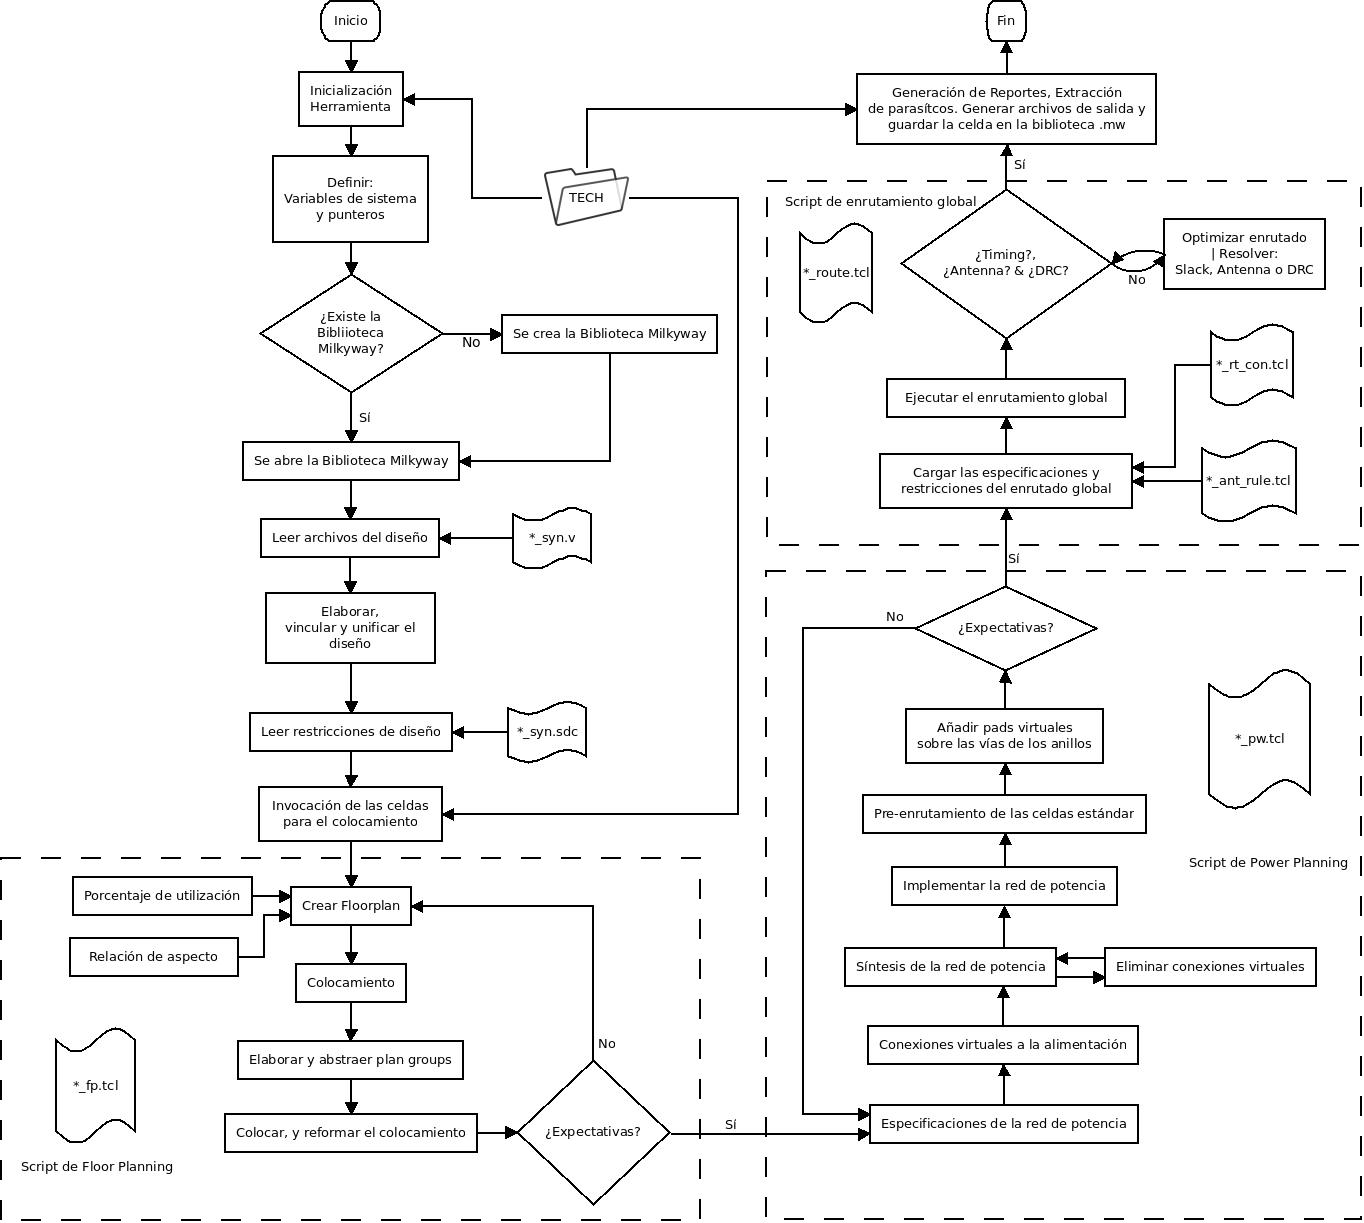
\includegraphics[width=\textwidth]{phy_syn.jpeg}
\centering
\caption{Diagrama de flujo que expone el proceso genérico de la implementación física en la herramienta \textit{IC Compiler}}
\label{fig:phy_script}
\end{figure}

\subsection{Script de simulación física: evaluación post implementación}

Al igual que en el proceso de síntesis es posible determinar la calidad de la implementación mediante el análisis de los reportes, y aunque hacer esto es importante, es necesario validar la funcionalidad del circuito mediante simulaciones \textit{Post-Place\&Route}.

El proceso no se detallará pues sigue la misma estructura que lo expuesto para la simulación post síntesis, en la sección \ref{sec:log_sim} y las diferencias fundamentales consisten en los punteros hacia los archivos fuente para la simulación. Lo cual pueda apreciarse claramente en la figura \ref{fig:phy_sim}.

\begin{figure}[ht]
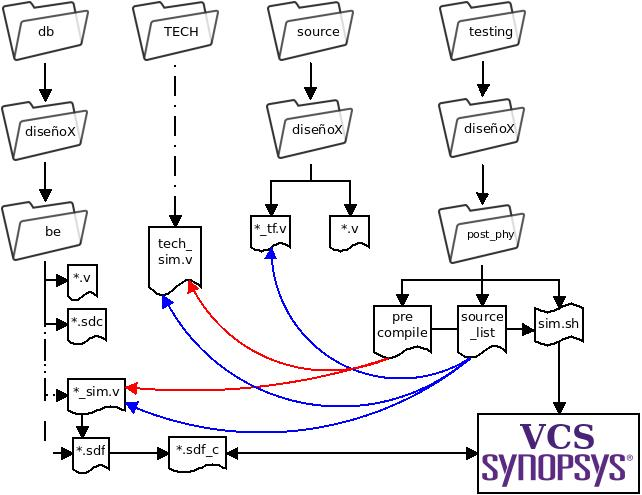
\includegraphics[scale=0.65]{post_phy_sim.jpeg}
\centering
\caption{Estructura del script de bash para la simulación post implementación}
\label{fig:phy_sim}
\end{figure}

\subsection{Script de Análisis de Sincronización Estática STA}
\label{sec:STA}

En esta sección se expone como se incorpora la herramienta \textit{PrimeTime} para evaluar si el diseño cumple las expectativas de sincronización de señales a la velocidad establecida en el diseño.

\textit{PrimeTime} es una herramienta que puede usarse tanto para evaluar un diseño post síntesis lógica como uno post implementación física. En el entorno mostrado en este documento se utiliza con mayor relevancia en la parte de \textit{BackEnd} del flujo pues sus resultados son más concluyentes, y es por ello que la herramienta es mencionada hasta esta sección; no obstante, puede incluirse como una etapa complementaria al flujo de \textit{FrontEnd}

\begin{figure}[ht]
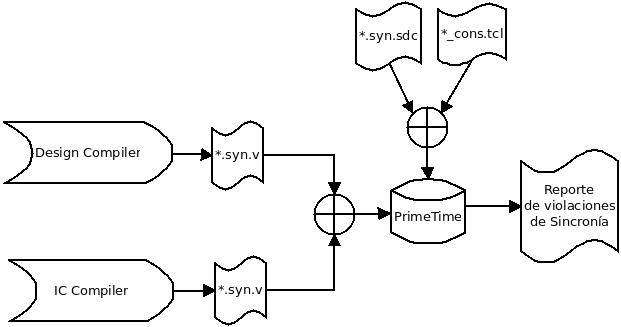
\includegraphics[scale=0.65]{Back_End_STA.jpeg}
\caption{Diagrama de flujo del análsis de sincronización estático}
\label{fig:staflow}
\end{figure}

Como se puede apreciar en la figura \ref{fig:staflow} el flujo de esta herramienta es bastante simple, para la misma se ha desarrollado un pequeño script, en este, como en todos los scripts mostrados hasta el momento, lo principal es inicializar la herramienta, definiendo los punteros hacia los archivos fuente y la biblioteca de la tecnología.

Luego de inicializar la herramienta se cargan los archivos fuente que consisten en: el archivo verilog con el \textit{GLN} implementado, el archivo \textit{SDF} con la información de los retardos de propagación a través del \textit{GLN}, el archivo \textit{SDC} con las restricciones de diseño de \textit{Synopsys} (principalmente las de sincronización), y finalmente el archivo \textit{SPEF} para incluir el efecto de las parasitancias en el análisis. También se pueden incluir otros archivos para realizar otros tipos de análisis como son archivos \textit{SAIF} que es un archivo que indica el factor de actividad de las celdas. De igual manera se puede estimular el diseño con otro conjunto de restricciones, estas corresponden con la misma sintaxis usada en el script de \textit{TCL} para definir las restricciones en la síntesis lógica (*\_cons.tcl).

Debido a que los diseños grandes y complejos presentan una enorme cantidad de restricciones, es necesario efectuar análisis multimodales y multiesquina\footnote{Multiesquina: Traducción literal de multicorner para referirse a que se evaluaran todas las condiciones esquina individualmente} \textit{PrimeTime} permite generar reportes enfocados a escenarios particures de sincronización. Ya sea para evaluar si el diseño cumple con las restricciones de diseño específicadas en una esquina o esquinas determinadas. \textit{PrimeTime} también permite hacer un análisis gráfico, y generar recomendaciones para alcanzar las restricciones de sincronización definidas; sin embargo, adentrar tan profundo en la herramienta está más allá del objetivo de este trabajo.

\begin{figure}[ht]
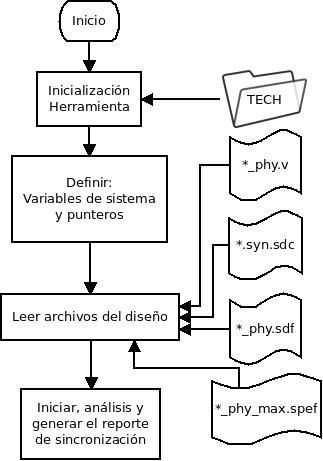
\includegraphics[scale=0.65]{phy_sta.jpeg}
\centering
\caption{Diagrama de flujo del script para un análisis básico de STA en la herramienta PrimeTime de Synopsys.}
\label{fig:stascript}
\end{figure}

El flujo de análisis expuesto en la figura \ref{fig:stascript}, expone un uso relativamente simple de la herramienta, generando un análisis sobre los 3 criterios más relevantes, retardos de entradas a registros, retardos entre registros y retardos de registros a salidas. Para los diseños trabajados en este proyecto, se considera una única condición de esquina, la cual corresponde a los valores típicos de retraso en las señales, una de tensión de 1.2v para las celdas estándar de la tecnología y a temperatura ambiental ($25^{\circ}C$). Estas condiciones se definen al inicializar la herramienta y cargar la biblioteca de la tecnología.

Los reportes generados usan motores similares a los que generan el análisis en las herramientas de síntesis; sin embargo, son más robustos en términos de profundidad y variedad en el análisis. Herramientas como \textit{Design Compiler} y \textit{IC Compiler} usan un modelado dinámico del diseño, valiéndose del peor escenario de propagación de señales, determinado mediante el modelo de Elmore. \textit{PrimeTime} permite usar modelos estáticos y es capaz de analizar distintos escenarios y estimular el diseño de diversas formas, para así evaluar el desempeño de la propagación de señales en distintos bloques de lógica, puramente combinacional, registros, puertos y/o distintas combinaciones de todos ellos.

\section{Script de síntesis de IP Cores y bibliotecas autónomas}
\label{sec:ip_syn}
Este apartado corresponde a una particularidad en el flujo de diseño digital propuesto, ya que no todos los diseños requieren incluir \textit{IPCores}\footnote{Un IPCore, o bloque de propiedad intelectual consiste en un módulo que no ofrece información sobre como es su arquitectura interna. Y su representación consiste en una caja negra. Esto con el fin de proteger la propiedad intelectual}, y la inclusión de los programas necesarios para su inclusión, irrumpe en la regularidad de la estructura de directorios definida anteriormente (ver inicio del capitulo \ref{ch:scripting}).

El flujo del diseño de las \textit{IP Cores}  requiere de 3 herramientas extra, la primera y principal corresponde al sintetizador de memorias de la tecnología utilizada, en este caso corresponde al software para la generación de : Artisan ARM Physical IP. Esta herramienta (Artisan) es un generador de \textit{IP Cores} para celdas de memorias (SRAM y ROM) del proceso IBM CMRF8SF-RVT, que es el proceso usado en este trabajo. La herramienta puede ser invocada a través de scripts, aunque también cuenta con una interfaz gráfica, bastante amigable.

Las 2 herramientas extra mencionadas pertenecen al conjunto de softwares de \textit{Synopsys}, y son el \textit{Library\_Compiler} y \textit{Milkyway}. El primero es necesario para definir una biblioteca lógica dedicada a los \textit{IPCores} y que el bloque SRAM generado pueda ser instanciado en el diseño y consecuente abstraído como un \textit{hardblock} en los procesos de síntesis. \textit{Milkyway} sirve como complemento para generar las bibliotecas físicas de las celdas.

No se expondrá mucho sobre el \textit{Library\_Compiler}, pues su uso es muy simple, y muy puntual. Esta herramienta es necesaria ya que al ejecutar Artisan, los productos de la síntesis de un \textit{IPCore} son archivos:

\begin{itemize}
\item Verilog, con el modelo \textit{GLN} para instanciar la celda generada. Algo equivalente a lo que se obtendría efectuando una síntesis lógica en \textit{DesignCompiler}.
\item dat, que es una tabla \textit{ASCII} con un resumen de la información geométrica y eléctrica de la celda.
\item PostScript, que es una pequeña hoja de datos con diagramas de sincronía e información sobre los puertos en formato ".ps".
\item VCLEF, este archivo contiene la información de la distribución de pads, diodos y metales para el enrutado (interconexión) y conexión externa en la celda.
\item CLF, es un archivo útil principalmente para las herramientas de \textit{Cadence} que es otro provedor de herramientas para diseño VLSI.  Sin embargo, los \textit{foundries} suelen solicitar este archivo por motivos de estandarización, así que conviene conservarlo. Contiene información relacionada con la antenas (Antenna) y los diodos de protección.
\item lib, acrónimo del formato liberty, que es un estándar para definir los parámetros de sincronía y potencia de la celda, así también como la conectividad con el exterior. Este archivo en conjunto al vclef permiten definir la celda física del \textit{IPCore}.
\item data, este es un archivo necesario para ejecutar el análisis \textit{STA} con \textit{PrimeTime}; sin embargo, requiere de una precompilación con un script de \textit{PERL} para generar correctamente el archivo \textit{.sdf}
\end{itemize}

Artisan permite generar más archivos de salida, para otra familia de herramientas como \textit{Cadence} por ejemplo; sin embargo, se han expuesto únicamente aquellos archivos relevantes para el flujo de diseño digital en cuestión, que se desarrolla en \textit{Synopsys}.

Teniendo claro lo anterior, es más fácil comprender cuál es el rol de las herramientas \textit{Library\_Compiler y Milkyway}, pues con ellos se generan las bibliotecas para el flujo.

\textit{Library\_Compiler} traduce la biblioteca en formato \textit{liberty (.lib)} al formato \textit{database (.db)} de \textit{Synopsys} con el fin de poder incluir la celda de memoria generada en el flujo \textit{FrontEnd}, en un diseño en particular. \textit{Milkyway} compila la información de la biblioteca de la tecnología, el archivo \textit{.vclef} y la biblioteca \textit{.db} (generada previamente por el \textit{Library\_Compiler}), para así desarrollar una nueva biblioteca \textit{.mw} que permita incluir la celda de memoria en el flujo \textit{BackEnd}, en un diseño en particular.

Las instrucciones necesarias para compilar la biblioteca en formato \textit{liberty} a una en formato \textit{database} son las siguientes, observe que la palabra library\_name se encuentra entre comillas, en este segmento se debe colocar el nombre de la biblioteca (sin comillas), el cual se definió al usar la herramienta \textit{Artisan}

\begin{lstlisting}[language= tcl, numbers=left, keywordstyle=\color{blue}, commentstyle=\color{mygreen}]
read_lib library.lib
write_lib "library_name" -format db -output library.db
\end{lstlisting}


El script para ejecutar la herramienta \textit{Milkyway} sigue un proceso similar al de la síntesis física. Primero se configuran los punteros y las bibliotecas de la tecnología. Luego se crea o se abre la biblioteca \textit{*.mw}, para incluir las nuevas celdas. Posteriormente al inicializar la biblioteca \textit{Milkyway} se leen los archivos \textit{.vclef}, aquí es importante destacar que la referencia un archivo particular de la tecnología (lefin\_layer\_map.txt) debe hacerse con cuidado. Este archivo contiene alias de los nombres de los metales de la tecnología, sin el es imposible generar de forma exitosa la biblioteca física. Los alias definidos en el archivo lefin\_layer\_map.txt deben ser congruentes con los nombres de los metales de la tecnología, de no ser así, deben ser editados. Este archivo debe incluirse ya que la herramienta \textit{Artisan} nombra de forma diferente a los metales cuando genera los archivos \textit{*.vclef}. Finalmente se leen los archivos \textit{.db} para actualizar la información de los puertos, en términos de la sincronía de las señales, etc. 

Como una consideración final, para mantener la regularidad, localidad y continuidad en los directorios y archivos, que se ha intentado establecer desde el principio, conviene tener una única biblioteca \textit{Milkyways} para los \textit{IP Cores}, así cada nueva macro celda se abstraerá de una única biblioteca auxiliar.

\begin{figure}[ht]
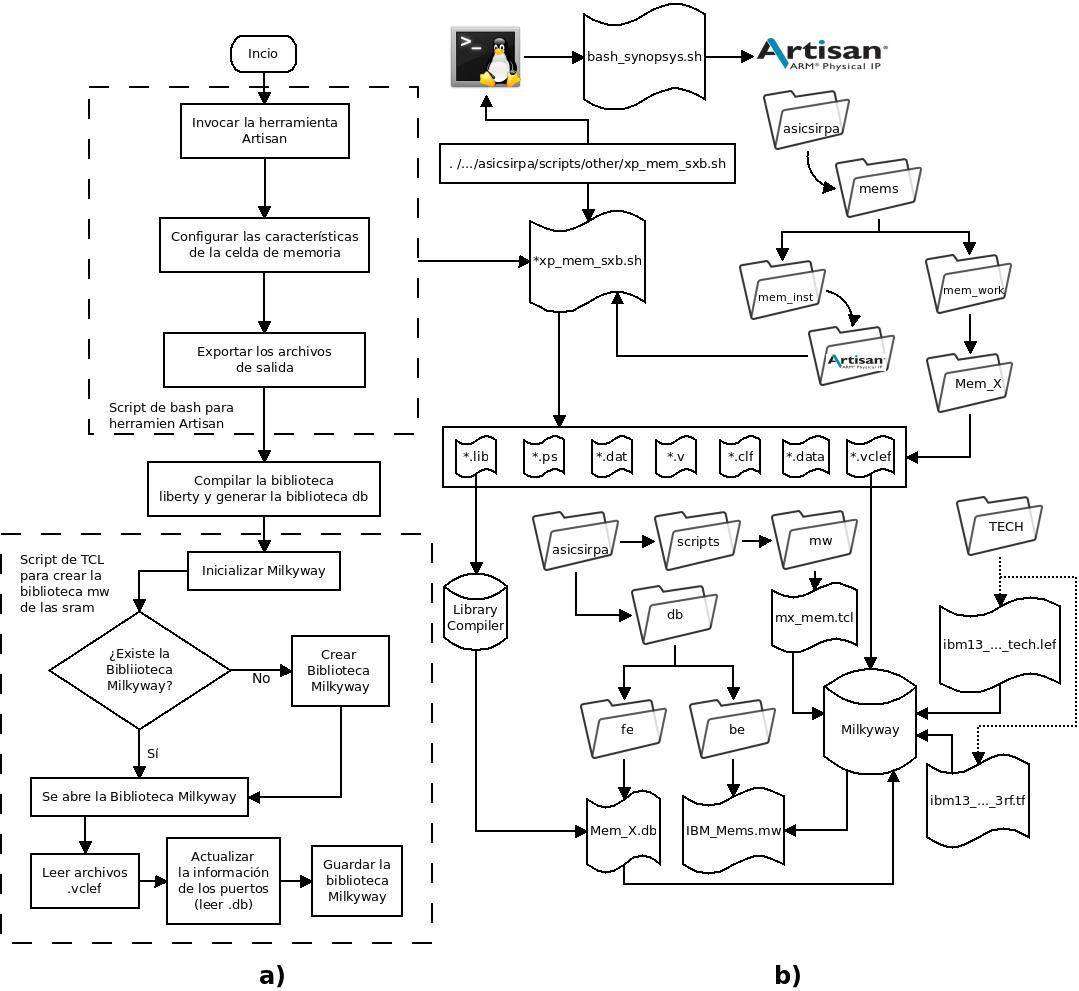
\includegraphics[width=\textwidth]{RAM_Syn.jpeg}
\centering
\caption{a) Diagrama de flujo de la síntesis de los \textit{IP Cores} de memorias SRAM y generación de las bibliotecas autónomas. \newline b) Estructura de directorios y archivos que intervienen en la síntesis de los IPcores de las memorias, herramientas involucradas y los archivos generados.}
\end{figure}

\newpage

\section{Análisis de resultados: Scripting }

En primera instancia cabe destacar que determinar la eficiencia de una estructura de directorios y archivos que pretenden realizar una tarea programática particular, depende de los paradigmas de trabajo individuales o de un equipo de trabajo. Por lo tanto no se puede establecer de forma cuantitativa que tan eficiente es la estructura de scripting que se planteó en este capítulo. En consecuencia este apartado se presenta como un análisis subjetivo y cualitativo del resultado obtenido en la experimentación con las herramientas de \textit{Synopsys} y la integración de un microprocesador \textit{RISC-V} para el proyecto \textit{SiRPA}.

Como se mencionó al inicio del capítulo, la forma en que los directorios y archivos fueron dispuestos responde a tres criterios, regularidad, localidad y continuidad. La estructura mostrada en la figura \ref{directorios} presenta una alta regularidad pues la mayoría de directorios tienen la misma jerarquía. Es continua, pues como puede observarse en las figuras \ref{beha_sim}, \ref{psyn_sim} y \ref{fig:phy_sim}, es posible rastrear los productos de los distintos procesos que afectan a los archivos. Finalmente, cuando un archivo es generado no es necesario, replicarlo en ningún otro directorio, los procesos que lo necesiten a posteriori pueden acceder a ellos mediante punteros, definidos en los scripts de los procesos que los requieran.

Finalmente quisiera declarar que lo expuesto en este capítulo tienen como sustento bibliográfico los manuales y páginas man de las herramientas de \textit{Synopsys}. La temática de la implementación del flujo digital respecto al \textit{Scripting} corresponden a una libre interpretación de la información contenida en estos manuales y las páginas man.









  \chapter{Síntesis lógica de un microprocesador RISC-V}
\label{ch:asp_syn}

En este capítulo se explica el proceso seguido para la sintetizar el código \textit{RTL} del microprocesador \textit{RISC-V} de aplicación específica desarrollado por el M.Sc. Carlos Salazar \cite{Carlosthesis}. En esencia la tarea encomendada consistía en efectuar la síntesis lógica del microprocesador y comprobar mediante simulaciones post síntesis su funcionabilidad.

\begin{figure}[t]
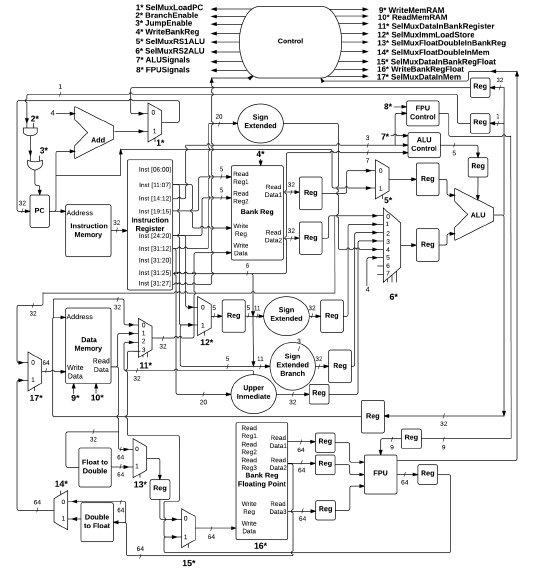
\includegraphics[width=\textwidth]{Micro.jpg}
\centering
\caption{Microprocesador ASP. RISC-V. Imágen replicada de \cite{Carlosthesis}, con la autorización del M.Sc Salazar.}
\label{fig:micro}
\end{figure}

\section{Escenario de implementación}

En la figura \ref{fig:micro}, observamos la estructura del microprocesador que debía ser síntetizado, el \textit{RTL} de este dispositivo mantiene una estructura equivalente a la de la figura \ref{fig:micro}; sin embargo, a primera impresión es posible encontrar una gran deficiencia en el diagrama de bloques mostrado. Esta deficiencia consiste en la ausencia de un hardware que permita cargarle información en las memorias. Al analizar el código del M.Sc. Salazar se encontró que las memorias utilizadas fueron definidas desde la persepectiva de ser usadas en una tarjeta de desarrollo \textit{FPGA}, este dispositivo permite cargar las memorias pues cuenta con hardware y software capacitado para dicho fin.

La estructura del \textit{RTL} de las memorias consiste en desarrollar pequeños bloques de memorias de 8 bits y generar un bloque de memoria total de 32 bits. La técnica de codificación usada corresponde a un arreglo bidimensional en verilog. En el caso de la memoria de programa o instrucciones, se crea un bloque de memoria de 32 Kbytes (kilo bytes), y se replica 4 veces para tener una memoria de 32 Kbytes con un tamaño de palabra de 32 bits, de forma similar sucede con la memoria de datos.

Sintetizar esta estructura de memorias en la herramienta es no es viable debido al enorme volumen de registros que se debe utilizar, y sin una estructura definida para guiar a la herramienta de síntesis, se obtendrá como resultado un \textit{GLN} deficiente. Es por ello que conviene incluir bloques de memoria SRAM, que correponde a una estructura de memoria más eficiente.

Considerando la meta del proyecto, la cual es desarrollar un ASIC de bajo consumo, integrar memorias tan grandes implica mal lograr el espacio de silicio disponible para el chip. Por otra parte ausencia del harware para programar las memorias compromete la correcta implementación del proyecto, pues las mismas aunque puedan ser sintetizadas por la herramienta, no podrán ser inicializadas de forma correcta, en etapas posteriores.

Existe una particularidad extra a este proyecto, y consiste en que la unidad de punto flotante original fue desarrollada por el Ing. Diego Rodríguez \cite{Diego2015}; sin embargo, el diseño tenía muchas oportunidades de mejora, es por ello que fue optimizada por el Ing. Francis López \cite{Francis2016}. Esta última no fue probada junto al microprocesador, aunque se demostró su funcionabilidad de forma individual.

Resolver los problemas asociados al banco de memoria del microprocesador y cualquier discrepancia de conectividad y sincronicidad del \textit{RTL} está más allá del alcance de este trabajo. Recordando el objetivo general de este trabajo, el cual es la implementación de un flujo de diseño digital en las herramientas de \textit{Synopsys} y para demostrar su funcionalidad se usa el \textit{RTL} del microprocesador en cuestión, es decir se pretende implementar el microprocesador ASP en una tecnología CMOS de 0,13 micrómetros, no se pretende garantizar la funcionalidad del mismo, la optimización del RTL está fuera de la visión de este trabajo.

\section{Estrategia de síntesis y validación}

Recordando, el primer objetivo específico de este trabajo, que corresponde a efectuar la síntesis lógica de el \textit{RTL} del \textit{ASP}, y habiendo definido en el capítulo \ref{ch:scripting} el flujo de diseño digital, se tiene en consecuencia que debe someterse el código \textit{RTL} a las herramientas de \textit{FrontEnd}. El flujo ya fue expuesto en el capítulo anterior, así que no se entrará en detalles sobre como fue sometido el código, pero se hablará de las configuraciones y consideraciones que se establecieron para que la implementación tenga coherencia con lo esperado del diseño.

\subsection{Restricciones del diseño}
\label{s_sec:const}

Lo expuesto a continuación corresponde a los criterios usados en el scritp de \textit{TCL} de constraints (restricciones) expuesto en la sección \ref{script_syn}. Y este es uno de los puntos de partida fundamentales para la síntesis lógica del ASP.

\subsubsection{Modelo de carga en el cableado (wire\_load\_model)}
El modelo de cableado utilizado en este diseño corresponde al ibm13\_wl10 de la biblioteca scx3\_cmos8rf\_lpvt\_tt\_1p2v\_25c. La forma para determinar los modelos de cableado se hace mediante la herramienta \textit{Design Compiler} y solicitando el reporte de la biblioteca; sin embargo, se debe tener funcionando de forma correcta el \textit{Library Compiler}. Existen varias modalidades de configuración para el modelo de cableado, en los diseños trabajados en este proyecto se utiliza el modelo "top".

En el modo superior "top", el compilador de diseño modela las redes como si el diseño no tuviese jerarquía y utiliza el modelo de carga de cable especificado para el nivel superior de la jerarquía de diseño de todas las redes en un diseño y sus subdiseños. La herramienta ignora todos los modelos de carga de cable configurados en subdiseños con el comando set\_wire\_load\_model.

\subsubsection{Reloj y factor de actividad}

Los diseños se diseñan previendo una frecuencia de operación general de 100 MHz por lo que se crea un reloj de con un periodo de 10 ns. Con el fin de modelar un reloj más realista se especifica una transición de 0.5 ns, lo cual se traduce como una pendiente en los flancos de subida y bajada del reloj.

También se específica una incertidumbre (skew) con márgenes de setup y de hold de 0.5 ns, esto corresponde al lapso entre dos flancos sucesivos con respecto a la variación fuera de los tiempos de llegada nominales. Finalmente se especifica una latencia de 0.5 ns, y es básicamente un parámetro que le indica a la herramienta el lapso que se da desde que la señal conmuta en su fuente hasta que conmuta en la entrada de una celda, y su utilidad es sólo para fines de análisis de sincronía y simulación dinámica.

Asociado indirectamente al reloj se encuentra el factor de actividad que le sirve a las herramientas, efectuar el análisis de potencia. Este parámetro se configura con una razón de conmutación del 25\% y una probabilidad estática del 50\% pues el reloj es simétrico.

\subsubsection{Puertos y propagación de señales}

Las señales de reloj y reset se configuran para que en ellas se coloquen la mínima cantidad de búfers, y que en general las señales se intervengan de forma mínima en la síntesis.

Se configura un intervalo de retraso en la propagación de los puertos, con el fin de que los análisis y la simulación sean más realistas, en el caso de las entradas el retardo es 1 ns como mínimo y de 3.5 ns como máximo, y de 1 a 2 ns para las salidas.

Los modelos de la carga asociada a las salidas y entradas se establecen en función de la celda de conducción (driving\_cell), esta configuración le permite a la herramienta de análisis de sincronía estimar de forma precisa el retraso causado desde la conmutación en un puerto, y sobre toda la ruta de propagación consecuente.

Se usa 10 la máxima cantidad de fanout permitda para los puertos de entrada, esto con el fin de que durante la síntesis la herramienta garantice que la cantidad de cargas conectadas directamente a esos puertos, no sobrepase un valor determinado.

\subsection{Comprobación de la síntesis}

Como ya se mencionó el diseño del M.Sc Salazar, presenta algunas deficiencias a la hora de considerar someterlo al flujo de diseño digital. En respuesta a lo anterior se efectuó el siguiente proceso.

\begin{enumerate}

\item En primer lugar se modificó el RTL haciendo un bypass\footnote{Bypass: anglicismo para aludir a un cambio de ruta o desvío en una ruta} en la conexión de la memorias, creando puertos para conectar de forma externa las memorias con los módulos que las instanciaban originalmente.

\item Se tomó el RTL original con la FPU diseñado por el Ing. Rodríguez, y se estimuló de acuerdo con el banco de pruebas (testbench) proporcionado junto al RTL del ASP. Esta simulación por comportamiento se define como la referencia dorada para validar el diseño.

\item Luego se sustituye la FPU por la diseñada por el Ing. López y se estimula el ASP de nuevo en una simulación por comportamiento para valorar la congruencia con el diseño original.

\item Se sintetiza entonces el RTL sin el banco de memorias, ya que como se mencionó anteriormente, incluir las memorias tal cual se diseñaron en la síntesis, es considerablemente engorroso e ineficiente.

\item Se realiza una simulación post síntesis lógica del ASP usando un estrategia de simulación hibrida, en el sentido de que se convinarán elementos de RTL (modelos por comportamiento) y elementos GLN (modelos post síntesis). Así se pretende modelar las memorias como elementos ideales y poder comprobar la funcionalidad del ASP.
\end{enumerate}

\section{Síntesis lógica del microprocesador ASP}

Habiendo definido el entorno particular en el que se recibió el RTL y las consideraciones que se tomaron para poder comprobar la correcta síntesis del mismo, se muestran los siguientes resultados ofrecidos por los reportes de la herramienta.

\begin{table}[ht]
\centering
\label{tab:qort}
\caption{QOR: Timing Path Group 'clk'}
\begin{tabular}{||l | c | c | c | c | c |}
\hline
\hline
Group & Internal & Switching  & Leakage & Total & \% Attrs \\
\hline
io\_pad & $0.0000$ & $0.0000$ & $0.0000$ & $0.0000$ & $(0.00\%)$ \\
\hline
memory & $0.0000$ & $0.0000$ & $0.0000$ & $0.0000$ & $(0.00\%)$ \\
\hline
black\_box & $0.0000$ & $0.0000$ & $0.0000$ & $0.0000$ & $(0.00\%)$\\
\hline
clock\_network & 4.0020e-02 & 0.4025 & 2.9799e+03 & 0.4425 & (35.67\%) \\
\hline
register & 0.5079 & 7.3101e-03 & 1.7763e+05 & 0.5154 & (41.55\%) \\
\hline
sequential  & 0.0000 & 0.0000 & 0.0000 & 0.0000 & (0.00\%) \\
\hline
combinational  3.5850e-02 & 0.2464 & 3.2011e+05 & 0.2826 & (22.78\%)
\hline
\hline
\end{tabular}
\end{table}

% \begin{table}[h]
% \centering
% \label{tab:01}
% \caption{blablabla}
% \begin{tabular}{
% @{\hspace{0cm}}|p{1.5cm} @{\hspace{0cm}}|p{1.2cm} @{\hspace{0cm}}|p{2cm}| @{\hspace{0cm}}|p{2.2cm}|}}
% \hline
% A & B & C & D\\
% \hline
% \end{tabular}
% \end{table}








  \chapter{Implementación física de la FPU del ASP y bloques de memoria}

Esta sección expone el proceso de evaluación del flujo digital correspondiente a la sección de "back end" sometiendo al flujo los componentes \textit{RTL} de una unidad aritmética en punto flotante (\textit{FPU}) que ejecuta operaciones de suma y multiplicación con signo, en precisión simple según el estándar IEEE574. Así mismo se somete al flujo dos \textit{IP Cores} correspondientes a bloques de memoria SRAM.

Respecto a la \textit{FPU} se usa el \textit{RTL} del diseño del Ing. López \cite{Francis2016}, este diseño fue implementado en 3 etapas, realizando una integración jerárquica, la primera corresponde a la síntesis lógica de los 2 módulos principales (suma y multiplicación) y la evaluación post síntesis de las mismas, la segunda etapa consiste en la integración física de cada unidad por separado, y posteriormente se efectúa una evaluación post implementación. Por último se integra el siguiente nivel en la jerarquía, el cual es el módulo principal que instancia los otros dos módulos mencionados.

Tanto la síntesis lógica como física siguen el proceso descrito en el capítulo anterior, según las secciones \ref{sec:syn_s} y \ref{sec:phy_s} respectivamente. Las restricciones consideradas para el proceso de front end y consecuentemente los scripts para la síntesis lógica son las mismas que las mostradas en la sección \ref{s_sec:const}, por lo que no se redundará en esos aspectos.

Respecto a la síntesis física, se consideraron las siguientes configuraciones para la síntesis del árbol de reloj:

\begin{itemize}
\item Inserción de celdas frontera cercanas a los puertos de reloj para el diseño basado en jerarquía de bloques.
\item OCV\_Clustering, para mejorar la distribución del reloj a través de ramas de registros. 
\item Finalmente permitir la re-ubicación y el re-dimensionamiento de las compuertas y \textit{búfers} para optimizar la síntesis del árbol de reloj.
\end{itemize}

Las reglas de antena tienen los siguientes atributos:
\begin{itemize}
\item Modalidad de protección de diodo limitada.
\item Una razón de metal de 150, un tamaño de compuerta por defecto de 0.1, con una protección por defecto de 0.5.
\item Un radio de corte de 20, y una razón de diodo comprendida en el siguiente vector \{0.09 0 123 16880\} para los metales de las capas bajas(4 primeras capas de metal), mientras que para las vías de estos primeros 4 metales el vector sería \{0.09 0 110 500\}
\end{itemize}

Respecto al enrutado global no hay una serie de restricciones o configuraciones específicas para que la herramienta logre enrutar de forma adecuada toda la celda, este proceso es algo engorroso, y responde más a una metodología iterativa y de optimización selectiva de acuerdo con los resultados que se van dando al trabajar con el layout del diseño. Sin embargo, se especifican parámetros como la reducción del efecto \textit{Crosstalk} para que en el enrutado se eviten colocar cables largos adyacentes a rieles paralelos, y tener un esfuerzo alto al controlar la ejecución de enrutamiento detallado e iterativo para determinar que el \textit{DRC} diverge.

En relación con los \textit{IP Cores} de las memorias, se efectuó un flujo equivalente, no obstante los \textit{IP Cores} no pueden ser optimizados ni trabajados en detalle, pues precisamente son cajas negras que buscan la protección de la propiedad itelectual. Así que la metodología para corroborar que la implementación de estos bloques fue correcta se evaluaron diseños que hacen de caparazón para estas celdas, en inglés a esta técnica se le conoce como \textit{"Wrapper"} y en esencia consiste en crear un diseño que use el \textit{IP Core} como una instancia y se sintetiza con base en él.

\section{Resultados de la síntesis lógica de la FPU}
\label{sec:fpu_syn_result}
En esta sección únicamente serán presentados los resultados obtenidos de la síntesis todo el bloque de la FPU pues incluir los resultados previos de los módulos de suma/resta y multiplicación sería redundante.

En la figura \ref{fig:fpu_cell} se muestra el resultado de la implementación de la unidad aritmética de punto flotante en la tecnología IBM 0.13 según el flujo de diseño establecido en este trabajo.

\begin{figure}[h]
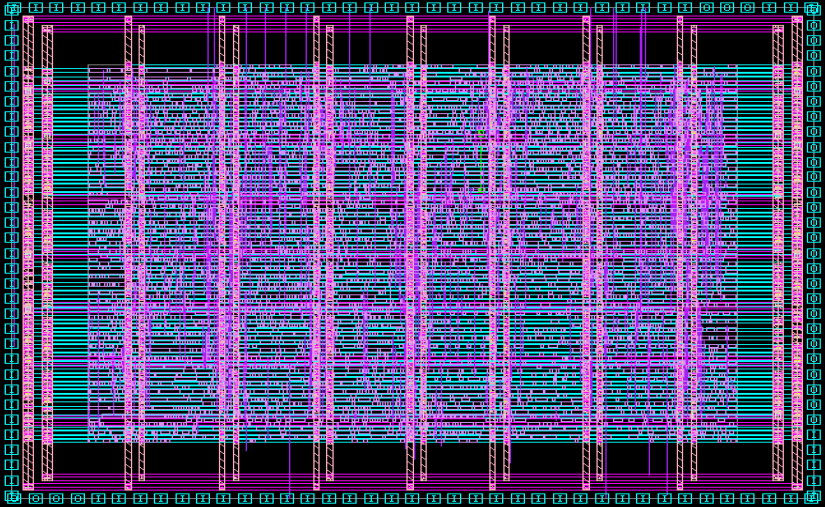
\includegraphics[width=\textwidth]{fpu_cell.png}
\centering
\caption{Foto captura del layout de la celda física generada para la unidad de punto flotante del ASP}
\label{fig:fpu_cell}
\end{figure}

\subsection{Reportes de síntesis lógica}
\label{s_sec:fpu_syn_report}

Al igual que en el capítulo anterior en este apartado se ofrece un resumen de los reportes más relevantes que ofrece la herramienta para evaluar el desempeño del diseño en términos de área, consumo de energía y sincronización de señales. Presentar datos sobre las celdas y los puertos  ofrecen información útil para efectuar un analisis más conciente sobre la administración de los recursos de la tecnología; sin embargo, esta por fuera del enfoque de este trabajo.\\

\newpage
\begin{table}[ht]
\centering
\label{tab:fpu_pwr_tb}
\caption{Resumen del reporte de potencia de la FPU post síntesis lógica}
\begin{tabular}{||l | c | c | c | c | c |}
\hline
\hline
Group & Internal & Switching  & Leakage & Total & \% Attrs \\
\hline
io\_pad & 0.0000 & 0.0000 & 0.0000 & 0.0000 & 0.00\% \\
\hline
memory & 0.0000 & 0.0000 & 0.0000 & 0.0000 & 0.00\% \\
\hline
black\_box & 0.0000 & 0.0000 & 0.0000 & 0.0000 & 0.00\% \\
\hline
clock\_network & 0.0000 & 0.0000 & 0.0000 & 0.0000 & 0.00\% \\
\hline
register & 1.2521 & 0.1130 & 2.4467e+04 & 1.3651 & 60.92\%\\
\hline
sequential  & 0.0000 & 0.0000 & 0.0000 & 0.0000 & 0.00\% \\
\hline
combinational & 0.2211 & 0.6546 & 5.0897e+04 & 0.8757 & 39.08\% \\
\hline
Total &  1.4732 mW & 0.7675 mW & 75.364e+04 nW & 2.2408 mW & 100\%\\
\hline
\hline
\end{tabular}
\end{table}

\begin{lstlisting}[caption={Reporte de área de la unidad de punto flotante de ASP post síntesis lógica.} \label{lst:fpu_area_report}, frame={single}]
****************************************
Report : area
Design : FloatingPointUnit
Version: L-2016.03-SP3
Date   : Tue Jan  3 18:53:58 2017
****************************************

	Library(s) Used: scx3_cmos8rf_lpvt_tt_1p2v_25c

          Number of ports:                          355
          Number of nets:                          5590
          Number of cells:                         4909
          Number of combinational cells:           4227
          Number of sequential cells:               680
          Number of macros/black boxes:               0
          Number of buf/inv:                        792
          Number of references:                      54

          Combinational area:              41843.520412
          Buf/Inv area:                     3906.720098
          Noncombinational area:           20897.279408
          Macro/Black Box area:                0.000000
          Net Interconnect area:          588843.014587

          Total cell area:                 62740.799820
          Total area:                     651583.814407
\end{lstlisting}

\newpage

\begin{lstlisting}[caption={Reporte de sincronía de la FPU post síntesis lógica.} \label{lst:fpu_timing_report}, frame={single},basicstyle=\small]
****************************************
Report : timing -path full -delay max -max_paths 1
Design : FloatingPointUnit Version: L-2016.03-SP3
****************************************
		Path Group: clk | Path Type: max
	
    Startpoint:FPU_Multiplication_Function/Operands_load_reg/
    XMRegister/Q_reg[21](rising edge-triggered flip-flop 
    clocked by CLK)
    Endpoint:FPU_Multiplication_Function/Sgf_operation/SgfM_mul_0.left/
    pdt_int_reg[23](rising edge-triggered flip-flop clocked by CLK)
  -------------------------------------------------------------------
  Des/Clust/Port     Wire Load Model       	Library
  FloatingPointUnit	ibm13_wl10     scx3_cmos8rf_lpvt_tt_1p2v_25c
  -------------------------------------------------------------------
  Point							Incr	Path
  clock CLK (rise edge)					0.00	0.00
  clock network delay (ideal)				1.00	1.00
  FPU_Multiplication_Function/Operands_load_reg/
  XMRegister/Q_reg[21]/CK (DFFRX4TS)			0.00	1.00 r
  FPU_Multiplication_Function/Operands_load_reg/
  XMRegister/Q_reg[21]/QN (DFFRX4TS)			1.18	2.18 r
  FPU_Multiplication_Function/U856/Y(INVX2TS)		0.27	2.45 f
  FPU_Multiplication_Function/U1080/Y(CLKXOR2X2TS)	0.63	3.08 f
  FPU_Multiplication_Function/U524/Y (INVX2TS)		0.46	3.54 r
  FPU_Multiplication_Function/U1071/Y (AND2X2TS)	0.48	4.02 r
  FPU_Multiplication_Function/U554/Y (INVX3TS)		0.25	4.27 f
  FPU_Multiplication_Function/U2192/Y (OAI22X1TS)	0.39	4.66 r
  FPU_Multiplication_Function/U2193/S (CMPR32X2TS)	0.75	5.42 f
  FPU_Multiplication_Function/mult_x_22/U195/
  S(CMPR42X2TS)						0.98	6.39 f
  FPU_Multiplication_Function/mult_x_22/U194/
  S(CMPR42X1TS)						1.19	7.58 f
  FPU_Multiplication_Function/U2107/Y(NAND2X1TS)	0.59	8.17 r
  FPU_Multiplication_Function/U2109/Y(OAI21X1TS)	0.51	8.68 f
  FPU_Multiplication_Function/U2110/Y(AOI21X2TS)	0.33	9.02 r
  FPU_Multiplication_Function/U2111/Y(OAI21X4TS)	0.24	9.26 f
  FPU_Multiplication_Function/U2121/Y(AOI21X4TS)	0.29	9.55 r
  FPU_Multiplication_Function/U726/Y(OAI21X4TS)		0.22	9.77 f
  FPU_Multiplication_Function/U725/Y(AOI21X2TS)		0.29	10.06 r
  FPU_Multiplication_Function/U1062/Y(XOR2X2TS)		0.28	10.34 r
  FPU_Multiplication_Function/Sgf_operation/
  SgfM_mul_0.left/pdt_int_reg[23]/D(DFFQX1TS)		0.00	10.34 r
  
  data arrival time						10.34
  
  clock CLK (rise edge)					10.00	10.00
  clock network delay (ideal)				1.00	11.00
  clock uncertainty					-0.50	10.50
  FPU_Multiplication_Function/Sgf_operation/
  SgfM_mul_0.left/pdt_int_reg[23]/CK(DFFQX1TS)		0.00	10.50 r
  library setup time					-0.16	10.34
  data required time						10.34
  -------------------------------------------------------------------
  data required time						10.34
  data arrival time						-10.34
  -------------------------------------------------------------------
  slack (MET)							0.00
  -------------------------------------------------------------------
  
  Startpoint:FPU_Add_Subtract_Function/Oper_Start_in_module/
  ASRegister/Q_reg[0](rising edge-triggered flip-flop 
  clocked by clk)
  Endpoint:FPU_Add_Subtract_Function/Add_Subt_Sgf_module/
  Add_overflow_Result/Q_reg[0]
  (rising edge-triggered flip-flop clocked by clk)
    
  -------------------------------------------------------------------
  Des/Clust/Port     Wire Load Model       	Library
  FloatingPointUnit	ibm13_wl10     scx3_cmos8rf_lpvt_tt_1p2v_25c
  -------------------------------------------------------------------
  Point							Incr	Path
  clock CLK (rise edge)					0.00	0.00
  clock network delay (ideal)				1.00	1.00
  FPU_Add_Subtract_Function/Oper_Start_in_module/
  ASRegister/Q_reg[0]/CK (DFFRX1TS)			0.00	1.00 r
  FPU_Add_Subtract_Function/Oper_Start_in_module/
  ASRegister/Q_reg[0]/Q (DFFRX1TS)			1.17	2.17 f
  FPU_Add_Subtract_Function/U1634/Y (CLKXOR2X4TS)	0.60	2.77 f
  FPU_Add_Subtract_Function/U1102/Y (XOR2X2TS)		0.40	3.17 r
  FPU_Add_Subtract_Function/U1130/Y (NAND2X4TS)		0.43    3.59 f
  FPU_Add_Subtract_Function/U1835/Y (INVX4TS)		0.46	4.05 r
  FPU_Add_Subtract_Function/U1839/Y (XOR2X1TS)		0.68	4.73 r
  FPU_Add_Subtract_Function/U1848/Y (INVX2TS)		0.39	5.11 f
  FPU_Add_Subtract_Function/U1849/Y (NOR2X1TS)		0.61	5.72 r
  FPU_Add_Subtract_Function/U1852/Y (AOI21X2TS)		0.50	6.23 f
  FPU_Add_Subtract_Function/U871/Y (OAI21X2TS)		0.43	6.65 r
  FPU_Add_Subtract_Function/U1436/Y (AOI21X2TS)		0.38	7.04 f
  FPU_Add_Subtract_Function/U1913/Y (OAI21X4TS)		0.31	7.34 r
  FPU_Add_Subtract_Function/U1917/Y (AOI21X4TS)		0.22	7.57 f
  FPU_Add_Subtract_Function/U1921/Y (OAI21X4TS)		0.27	7.83 r
  FPU_Add_Subtract_Function/U1925/Y (AOI21X4TS)		0.22	8.06 f
  FPU_Add_Subtract_Function/U1929/Y (OAI21X4TS)		0.27	8.32 r
  FPU_Add_Subtract_Function/U1933/Y (AOI21X4TS)		0.22	8.55 f
  FPU_Add_Subtract_Function/U1937/Y (OAI21X4TS)		0.27	8.82 r
  FPU_Add_Subtract_Function/U1941/Y (AOI21X4TS)		0.22	9.04 f
  FPU_Add_Subtract_Function/U1945/Y (OAI21X4TS)		0.25	9.29 r
  FPU_Add_Subtract_Function/U1962/Y (AOI21X2TS)		0.21	9.50 f
  FPU_Add_Subtract_Function/U895/Y (XOR2X2TS)		0.28	9.78 r
  FPU_Add_Subtract_Function/U1963/Y (CLKMX2X2TS)	0.41	10.20 r
  FPU_Add_Subtract_Function/Add_Subt_Sgf_module/
  Add_overflow_Result/Q_reg[0]/D (DFFRX2TS)		0.00	10.20 r
  
  data arrival time						10.20

  clock clk (rise edge)					10.00	10.00
  clock network delay (ideal)				1.00	11.00
  clock uncertainty					-0.50	10.50
  FPU_Add_Subtract_Function/Add_Subt_Sgf_module/
  Add_overflow_Result/Q_reg[0]/CK (DFFRX2TS)		0.00	10.50 r
  library setup time					-0.30	10.20
  data required time						10.20
  -------------------------------------------------------------------
  data required time						10.34
  data arrival time						-10.34
  -------------------------------------------------------------------
  slack (MET)							0.00
  ------------------------------------------------------------------
\end{lstlisting}

\subsection{Reportes de síntesis física}
\begin{table}[ht]
\centering
\label{tab:fpu_pwr_p_tb}
\caption{Resumen del reporte de potencia de la FPU post síntesis física}
\begin{tabular}{||l | c | c | c | c | c |}
\hline
\hline
Group & Internal & Switching  & Leakage & Total & \% Attrs \\
\hline
io\_pad & 0.0000 & 0.0000 & 0.0000 & 0.0000 & 0.00\% \\
\hline
memory & 0.0000 & 0.0000 & 0.0000 & 0.0000 & 0.00\% \\
\hline
black\_box & 0.0000 & 0.0000 & 0.0000 & 0.0000 & 0.00\% \\
\hline
clock\_network & 0.0000 & 0.0000 & 0.0000 & 0.0000 & 0.00\% \\
\hline
register & 1.2530 & 4.7273e-02 & 2.4587e+04 & 1.3003 & 78.51\%\\
\hline
sequential  & 0.0000 & 0.0000 & 0.0000 & 0.0000 & 0.00\% \\
\hline
combinational & 0.1274 & 0.2285 & 5.1105e+04 & 0.3560 & 21.49\% \\
\hline
Total &  1.3804 mW & 0.2758 mW & 75.692e nW & 1.6563 mW & 100\%\\
\hline
\hline
\end{tabular}
\end{table}

\newpage

\begin{lstlisting}[caption={Reporte de área de la unidad de punto flotante de ASP post síntesis lógica.} \label{lst:fpu_area_p_report}, frame={single}]
****************************************
Report : area
Design : FloatingPointUnit
Version: L-2016.03-SP3
Date   : Tue Jan  3 18:53:58 2017
****************************************

	Library(s) Used: scx3_cmos8rf_lpvt_tt_1p2v_25c

          Number of ports:                          144
          Number of nets:                           825
          Number of cells:                          646
          Number of combinational cells:            513
          Number of sequential cells:               131
          Number of macros/black boxes:               0
          Number of buf/inv:                        136
          Number of references:                      63

          Combinational area:              42115.680429
          Buf/Inv area:                     4190.400109
          Noncombinational area:           20897.279408
          Macro/Black Box area:                0.000000
          Net Interconnect area:              undefined
                               (No wire load specified)

          Total cell area:                 63012.959836
          Total area:                 undefined
\end{lstlisting}

\begin{lstlisting}[caption={Reporte de sincronía del microprocesador ASP post síntesis lógica.} \label{lst:fpu_timing_p_report}, frame={single},basicstyle=\small]
**************************************************
Report : timing -path full -delay max -max_paths 1
Design : FloatingPointUnit Version: L-2016.03-SP3
**************************************************
Operating Conditions: tt_1p2v_25c
Library: scx3_cmos8rf_lpvt_tt_1p2v_25c
	Parasitic source    : LPE
	Parasitic mode      : RealRC
	Extraction mode     : MIN_MAX
	Extraction derating : 25/25/25
	
    Startpoint: FPU_Multiplication_Function/Operands_load_reg/
    XMRegister/Q_reg[10](rising edge-triggered flip-flop clocked
    by CLK)
    Endpoint:FPU_Multiplication_Function/Sgf_operation/
    SgfM_mul_0.middle/pdt_int_reg[15](rising edge-triggered 
    flipflop clocked by CLK)
    
    		Path Group: clk | Path Type: max
  -------------------------------------------------------------------
  Des/Clust/Port     Wire Load Model       	Library
  FloatingPointUnit	ibm13_wl10     scx3_cmos8rf_lpvt_tt_1p2v_25c
  -------------------------------------------------------------------
  Point							Incr	Path
  clock CLK (rise edge)					0.00	0.00
  clock network delay (ideal)				1.00	1.00
  FPU_Multiplication_Function/Operands_load_reg/
  XMRegister/Q_reg[10]/CK (DFFRX4TS)			0.00	1.00 r
  FPU_Multiplication_Function/Operands_load_reg/
  XMRegister/Q_reg[10]/QN (DFFRX4TS)			0.88	1.88 f
  FPU_Multiplication_Function/U1092/Y (INVX2TS)		0.44 &	2.32 r
  FPU_Multiplication_Function/U1766/Y (CLKXOR2X2TS)	0.58 &	2.90 f
  FPU_Multiplication_Function/U1767/Y (NOR2X2TS)	0.18 &	3.08 r
  FPU_Multiplication_Function/U1211/Y (XOR2X1TS)	0.49 &	3.56 r
  FPU_Multiplication_Function/U1191/Y (NAND2X6TS)	0.35 &	3.92 f
  FPU_Multiplication_Function/U2505/Y (OAI22X1TS)	0.59 &	4.51 r
  FPU_Multiplication_Function/U1066/S (CMPR32X2TS)	1.06 &	5.57 f
  FPU_Multiplication_Function/DP_OP_110J1_122_5487/
  U307/CO (CMPR42X1TS)					1.15 &	6.73 f
  FPU_Multiplication_Function/DP_OP_110J1_122_5487/
  U303/S (CMPR42X2TS)					1.01 &	7.74 f
  FPU_Multiplication_Function/U1593/Y (NOR2X4TS)	0.18 &	7.92 r
  FPU_Multiplication_Function/U1594/Y (NOR2X2TS)	0.14 &	8.06 f
  FPU_Multiplication_Function/U1596/Y (AOI21X4TS)	0.33 &	8.39 r
  FPU_Multiplication_Function/U408/Y (INVX2TS)		0.22 &	8.61 f
  FPU_Multiplication_Function/U1607/Y (AOI21X1TS)	0.22 &	8.82 r
  FPU_Multiplication_Function/U1051/Y (XOR2X1TS)	0.46 &	9.28 r
  FPU_Multiplication_Function/Sgf_operation/
  SgfM_mul_0.middle/pdt_int_reg[15]/D (DFFQX1TS)	0.00 &	9.28 r
  
  data arrival time						9.28

  clock CLK (rise edge)					10.00	10.00
  clock network delay (ideal)				1.00	11.00
  clock uncertainty					-0.50	10.50
  FPU_Multiplication_Function/Sgf_operation/
  SgfM_mul_0.middle/pdt_int_reg[15]/CK (DFFQX1TS)	0.00	10.50 r
  library setup time					-0.27	10.23
  data required time						10.23
  ------------------------------------------------------------------
  data required time						10.23
  data arrival time						-9.28
  ------------------------------------------------------------------
  slack (MET)							0.94
  
  Startpoint:FPU_Add_Subtract_Function/Oper_Start_in_module/
  YRegister/Q_reg[31](rising edge-triggered flip-flop clocked by clk)
  
  Endpoint:FPU_Add_Subtract_Function/Add_Subt_Sgf_module/
  Add_Subt_Result/Q_reg[24](rising edge-triggered flip-flop
  clocked by clk)
  
  			Path Group: clk | Path Type: max

  Point							Incr	Path
  clock clk (rise edge)					0.00	0.00
  clock network delay (ideal)           		1.00	1.00
  FPU_Add_Subtract_Function/Oper_Start_in_module/
  YRegister/Q_reg[31]/CK (DFFRX1TS)			0.00	1.00 r
  FPU_Add_Subtract_Function/Oper_Start_in_module/
  YRegister/Q_reg[31]/Q (DFFRX1TS)			1.10	2.10 f
  FPU_Add_Subtract_Function/U1634/Y (CLKXOR2X4TS)	0.45 &	2.55 f
  FPU_Add_Subtract_Function/U1102/Y (XOR2X2TS)		0.35 &	2.91 r
  FPU_Add_Subtract_Function/U1130/Y (NAND2X4TS)		0.34 &	3.25 f
  FPU_Add_Subtract_Function/U1129/Y (INVX8TS)		0.17 @  3.42 r
  FPU_Add_Subtract_Function/U1885/Y (XOR2X1TS)		0.43 @	3.85 r
  FPU_Add_Subtract_Function/U1901/Y (NAND2X1TS)		0.43 &	4.28 f
  FPU_Add_Subtract_Function/U880/Y (OAI21XLTS)		0.45 &	4.73 r
  FPU_Add_Subtract_Function/U1903/Y (AOI21X1TS)		0.25 &	4.98 f
  FPU_Add_Subtract_Function/U1904/Y (OAI21X2TS)		0.15 &	5.13 r
  FPU_Add_Subtract_Function/U1436/Y (AOI21X2TS)		0.16 &	5.29 f
  FPU_Add_Subtract_Function/U1913/Y (OAI21X4TS)		0.21 &	5.50 r
  FPU_Add_Subtract_Function/U1917/Y (AOI21X4TS)		0.15 &	5.65 f
  FPU_Add_Subtract_Function/U1921/Y (OAI21X4TS)		0.17 &	5.82 r
  FPU_Add_Subtract_Function/U1925/Y (AOI21X4TS)		0.13 &	5.95 f
  FPU_Add_Subtract_Function/U1929/Y (OAI21X1TS)		0.41 &	6.36 r
  FPU_Add_Subtract_Function/U1933/Y (AOI21X4TS)		0.27 &	6.63 f
  FPU_Add_Subtract_Function/U1937/Y (OAI21X1TS)		0.46 &	7.09 r
  FPU_Add_Subtract_Function/U1941/Y (AOI21X4TS)		0.30 &	7.39 f
  FPU_Add_Subtract_Function/U2006/Y (XOR2X1TS)		0.58 &	7.97 r
  FPU_Add_Subtract_Function/U905/Y (CLKMX2X2TS)		0.60 &	8.57 r
  FPU_Add_Subtract_Function/Add_Subt_Sgf_module/
  Add_Subt_Result/Q_reg[24]/D (DFFRX2TS)		0.00 &	8.57 r
  
  data arrival time						8.57

  clock clk (rise edge)					10.00	10.00
  clock network delay (ideal)				1.00	11.00
  clock uncertainty					-0.50	10.50
  FPU_Add_Subtract_Function/Add_Subt_Sgf_module/
  Add_Subt_Result/Q_reg[24]/CK (DFFRX2TS)		0.00	10.50 r
  library setup time					-0.28	10.22
  data required time						10.22
  -----------------------------------------------------------------
  data required time						10.22
  data arrival time						-8.57
  -----------------------------------------------------------------
  slack (MET)							1.65
\end{lstlisting}

\subsection{Reportes del análisis de sincronización estática (STA)}
\begin{lstlisting}[caption={Reporte STA de la FPU. Anotaciones sobre el análisis entre registros y puertos.} \label{lst:fpu_sta_n_report}, frame={single}]
              ****************************************
              Report : timing
                  -path_type full
                  -delay_type max
                  -slack_lesser_than 0.00
                  -max_paths 40
                  -sort_by slack
              Design : FloatingPointUnit
              Version: K-2015.06-SP3-3
              Date   : Mon Feb 13 16:21:27 2017
              ****************************************

              No paths with slack less than 0.00.
\end{lstlisting}


\begin{lstlisting}[caption={Reporte STA de la FPU. Anotaciones sobre el análisis entre registros y puertos.} \label{lst:fpu_sta_report}, frame={single},basicstyle=\small]
****************************************
Report : timing
	-path_type full
	-delay_type max
	-input_pins
	-nets
	-max_paths 1
	-transition_time
	-capacitance
	-sort_by slack
Design : FloatingPointUnit
Version: K-2015.06-SP3-3
Date   : Mon Feb 13 16:21:37 2017
****************************************


	Startpoint:FPU_Multiplication_Function/Operands_load_reg/
	XMRegister/Q_reg[10]
	(rising edge-triggered flip-flop clocked by CLK)
	Endpoint:FPU_Multiplication_Function/Sgf_operation/
	SgfM_mul_0.middle/pdt_int_reg[15]
	(rising edge-triggered flip-flop clocked by CLK)
		
        Path Group: CLK 	Path Type: max

  Point				Fanout	Cap	Trans	Incr	Path
  ----------------------------------------------------------------------
  clock CLK (rise edge)		--	--	0.50	0.00	0.00
  clock network delay (ideal)	--	--	----	1.00	1.00
  Operands_load_reg/XMRegister/
  Q_reg[10]/CK (DFFRX4TS)	--	--	0.00	0.00	1.00 r
  Operands_load_reg/XMRegister/
  Q_reg[10]/QN (DFFRX4TS)	--	--	0.00	0.88 *	1.88 f
  n576 (net)			2	0.01 
  U1092/A (INVX2TS)		--	--	0.00	0.00 *	1.88 f
  U1092/Y (INVX2TS)		--	--	0.00	0.44 *	2.32 r
  n435 (net)			9	0.08	---- 	----	----
  U1766/A (CLKXOR2X2TS)		--	----	0.00	0.00 *	2.32 r
  U1766/Y (CLKXOR2X2TS)		--	----	0.00	0.58 *	2.90 f
  n1110 (net)			2	0.01	----	----	-----
  U1767/B (NOR2X2TS)		--	----	0.00	0.00	*2.90 f
  U1767/Y (NOR2X2TS)		--	----	0.00	0.18 *	3.08 r
  n1108 (net)			1	0.01	----	----	----
  U1211/A (XOR2X1TS)		--	----	0.00	0.00 *	3.08 r
  U1211/Y (XOR2X1TS)		--	----	0.00	0.49 *	3.56 r
  n1116 (net)			1	0.02	----	----	----
  U1191/A (NAND2X6TS)		--	----	0.00	0.00 *	3.56 r
  U1191/Y (NAND2X6TS)		--	----	0.00	0.35 *	3.92 f
  n1906 (net)			10	0.04	----	----	----
  U2505/B0 (OAI22X1TS)		--	----	0.00	0.00 *	3.92 f
  U2505/Y (OAI22X1TS)		--	----	0.00	0.59 *	4.51 r
  n1910 (net)			1	0.02	----	----	---- 
  U1066/B (CMPR32X2TS)		--	----	0.00	0.00 *	4.51 r
  U1066/S (CMPR32X2TS)		--	----	0.00	1.06 *	5.58 f
  DP_OP_110J1_122_5487/n332(net) 1	0.01	----	----	----
  DP_OP_110J1_122_5487/
  U307/B (CMPR42X1TS)		--	----	0.00	0.00 *	5.58 f
  DP_OP_110J1_122_5487/
  U307/CO (CMPR42X1TS)		--	----	0.00	1.15 *	6.73 f
  DP_OP_110J1_122_5487/n329(net) 1	0.01	----	----	----
  DP_OP_110J1_122_5487/U303/
  C (CMPR42X2TS)		--	----	0.00	0.00 *	6.73 f
  DP_OP_110J1_122_5487/U303/
  S (CMPR42X2TS)		--	----	0.00	1.01 *	7.74 f
  DP_OP_110J1_122_5487/n319(net) 2	0.02	----	---- 
  U1593/A (NOR2X4TS)		--	----	0.00	0.00 *	7.74 f
  U1593/Y (NOR2X4TS)		--	----	0.00	0.18 *	7.92 r
  n1671 (net)			3	0.02	----	----	----
  U1594/A (NOR2X2TS)		--	----	0.00	0.00 *	7.92 r
  U1594/Y (NOR2X2TS)		--	----	0.00	0.14 *	8.06 f
  n976 (net)			1	0.01	----	----	---- 
  U1596/A1 (AOI21X4TS)		--	----	0.00	0.00 *	8.06 f
  U1596/Y (AOI21X4TS)		--	----	0.00	0.33 *	8.39 r
  n1104 (net)			2	0.04	----	----	---- 
  U408/A (INVX2TS)		--	----	0.00	0.00 *	8.39 r
  U408/Y (INVX2TS)		--	----	0.00	0.22 *	8.61 f
  n1669 (net)			4	0.01	----	----	---- 
  U1607/A0 (AOI21X1TS)		--	----	0.00	0.00 *	8.61 f
  U1607/Y (AOI21X1TS)		--	----	0.00	0.22 *	8.83 r
  n986 (net)			1	0.00	----	----	---- 
  U1051/A (XOR2X1TS)		--	----	0.00	0.00 *	8.83 r
  U1051/Y (XOR2X1TS)		--	----	0.00	0.46 *	9.28 r
  Sgf_operation/SgfM_mul_0.middle/
  N15(net)			1	0.02	----	----	----
  Sgf_operation/SgfM_mul_0.middle/
  pdt_int_reg[15]/D (DFFQX1TS)	--	----	0.00	0.00 *	9.29 r
  
  data arrival time		--	----	----	----	9.29

  clock CLK (rise edge)		--	----	0.50	10.00	10.00
  clock network delay (ideal)	--	----	----	1.00	11.00
  clock reconvergence pessimism	--	----	----	0.00	11.00
  clock uncertainty		--	----	----	-0.50	10.50
  Sgf_operation/SgfM_mul_0.middle/
  pdt_int_reg[15]/CK (DFFQX1TS)	--	----	-----	-----	10.50 r
  library setup time		--	----	----	-0.27 *	10.23
  data required time		---	----	----	----	10.23
  -----------------------------------------------------------------
  data required time		--	----	----	----	10.23
  data arrival time		--	----	----	----	-9.29
  -----------------------------------------------------------------
  slack (MET)			--	----	----	-----	0.94
  
  Note: All the points starts from FPU_Multiplication_Function/

\end{lstlisting}

\newpage

\subsection{Simulaciones}
\label{s_sec:fpu_sim}
Dado que en esta sección se analiza el comportamiento de módulos matemáticos, que en esencia brindan el resultado de operar dos datos con una función particular (suma, resta o multiplicación, con signo). Conviene usar una estrategia de verificación que tome la unidad bajo prueba y la estimule con vectores de datos leídos desde archivos fuente, y generar un vector de respuesta, con, valga la redundancia, los resultados de operar los elementos de los vectores de estímulo, y guardar este vector en otro archivo. Generar un vector con las respuestas a un estímulo determinado, permite comparar con mayor facilidad si el diseño ejecuta la función para la que fue concebido después del proceso de síntesis.

Dicho lo anterior este apartado se considera más productivo mostrar un análisis gráfico de los resultados de las simulaciones, pero no mediante diagramas de tiempo, si no realizando un contraste entre las respuestas a las distintas simulaciones, aprovechando el hecho de que la estrategia de simulación usada, en el testbench (aportado junto al \textit{RTL} de la FPU), consiste en estimular el diseño con un vector de datos leídos desde un archivo fuente, y guardando el vector de respuesta en otro archivo de texto. Mediante la herramienta \textit{Octave} es posible graficar la relación entre los datos.

El testbench para la FPU, ejercita una serie de pruebas para verificar que las funciones de los módulos son correctos, tiene 2 vectores de estímulo, y mediante un bucle se recorren los vectores estimulando el diseño y almacenando el resultado en un vector, en cada iteración. En total se ejecutan unas mil pruebas.

Se muestra el resultado de esas mil pruebas elaborando un gráfico de la siguiente manera: Se presenta 2 figuras con 3 gráficas (figuras \ref{fig:sim_add} y \ref{fig:sim_add} ), con el fin de no realizar demasiada contaminación visual, se les da un offset (desnivel) a los datos correspondientes a las simulaciones post síntesis, para verificar que tan similares son los resultados. El eje horizontal representa el índice de la muestra del vector de resultados, y el eje vertical muestra la magnitud, es decir el valor del resultado.

Como complemento a estas gráficas también se genera otro par de gráficas que muestran que tan desvidados se encuentran los datos de las simulaciones post síntesis respecto a los esperables según la simulación por comportamiento, que se ha tomado como la referencia dorada del diseño, en ausencia a otro modelo de alto nivel para tomar como referencia.

\newpage


\begin{figure}[h]
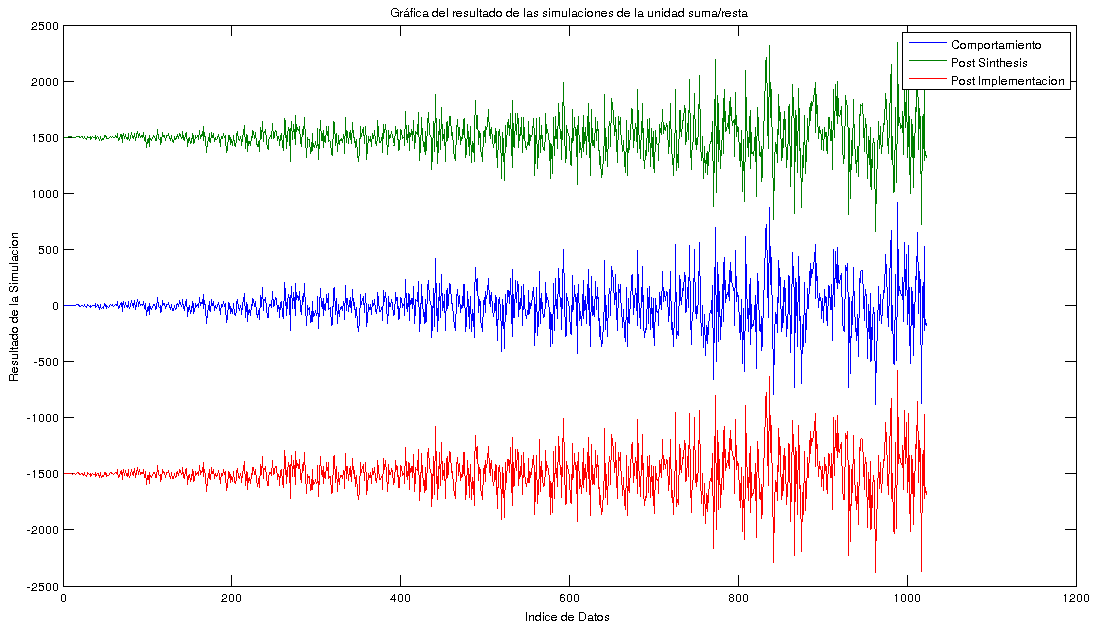
\includegraphics[width=\textwidth,height=8.5cm]{SimulacionADD.png}
\centering
\caption{Gráfico de los resultados de las distintas simulaciones asociadas con el módulo de suma y resta de la FPU. Observar que hay un desface entre los datos, hecho a drede para apreciar mejor la dinámica de las distintas gráficas.}
\label{fig:sim_add}
\end{figure}

\begin{figure}[h]
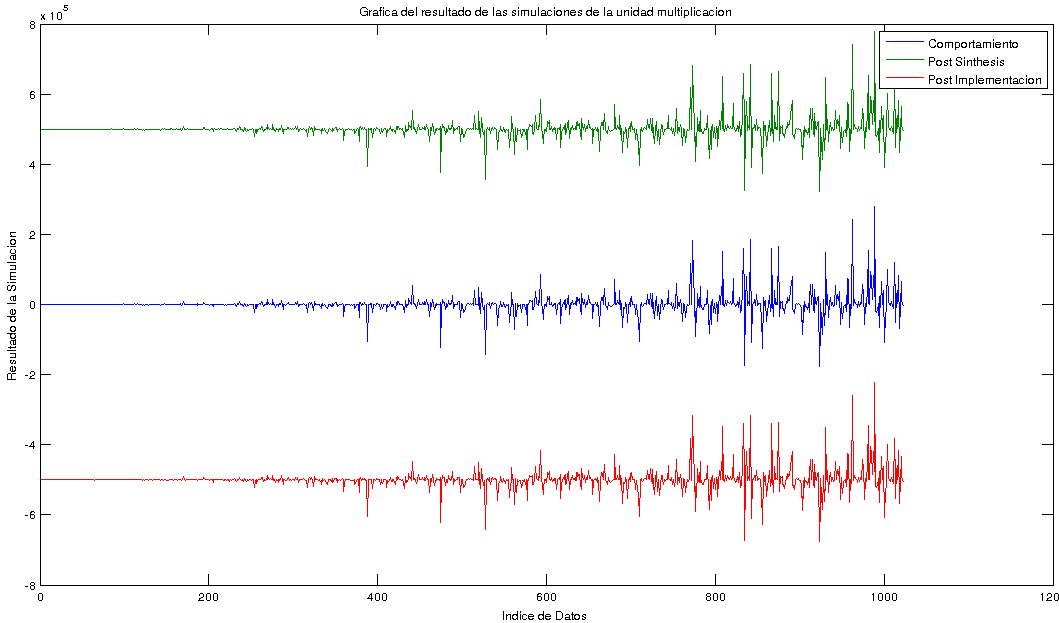
\includegraphics[width=\textwidth,height=9cm]{SimulacionMULT.png}
\centering
\caption{Gráfico de los resultados de las distintos simulaciones asociadas con el módulo de multiplicación con signo de la FPU Observar que hay un desface entre los datos, hecho a drede para apreciar mejor la dinámica de las distintas gráficas.}
\label{fig:sim_mult}
\end{figure}

\newpage


\begin{figure}[h]
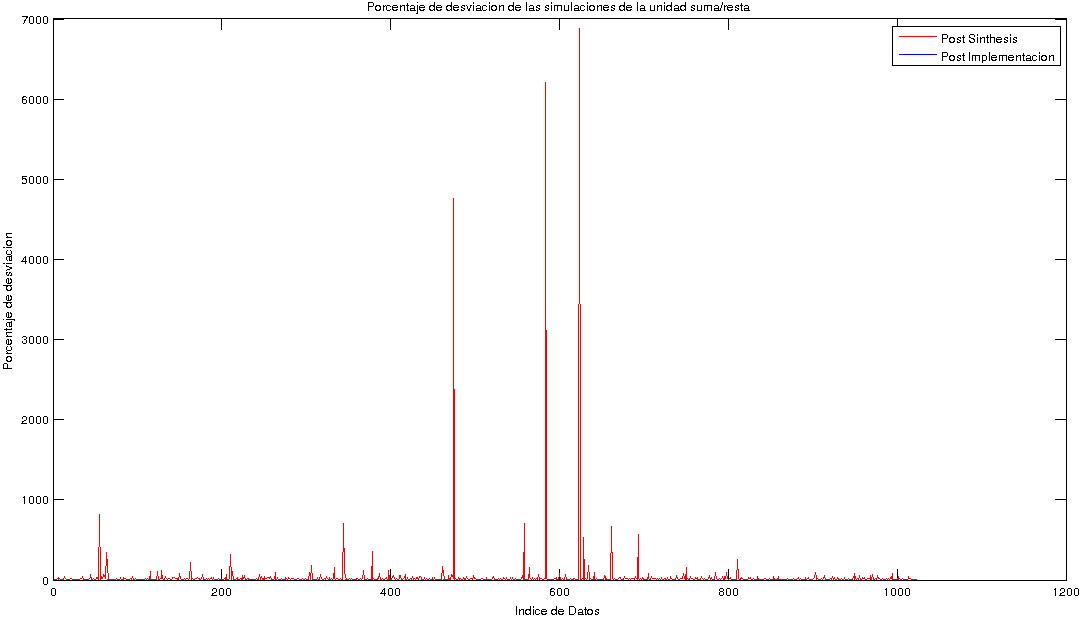
\includegraphics[width=\textwidth,height=8cm]{DesviacionADD.png}
\centering
\caption{Gráfica del porcentaje de desviación, de las simulaciones post síntesis de la unidad de suma y resta de la FPU, respecto a simulación por comportamiento. Se que la simulación post síntesis lógica, presenta algunas incongruencias para ciertos datos, mientras la síntesis física es congruente.}
\label{fig:desv_add}
\end{figure}

\begin{figure}[h]
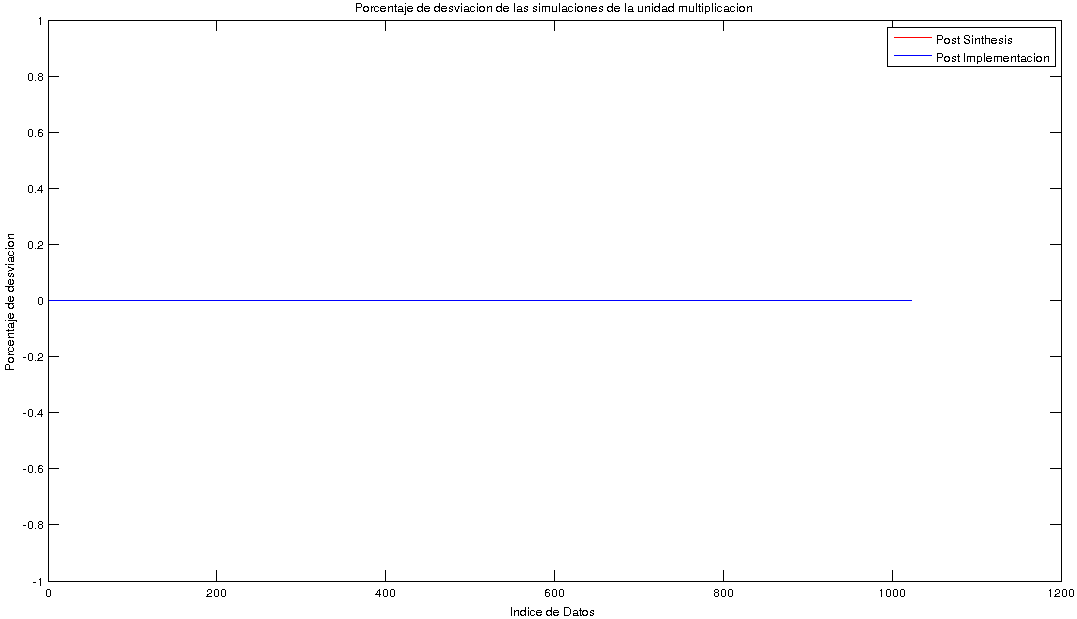
\includegraphics[width=\textwidth,height=8cm]{DesviacionMULT.png}
\centering
\caption{Gŕafica que muestra el porcentaje de desviación, de las simulaciones post síntesis de la unidad de multiplicación de la FPU. Observe que ambas líneas son perfectamente horizontales, lo que indica que la simulaciones post síntesis son consistentes con la de comportamiento}
\label{fig:desv_mult}
\end{figure}

\newpage

\subsection{Análisis de los resultados obtenidos en la implementación de la FPU}

\subsubsection{Potencia}
Comenzando por el análisis de los reportes de potencia post síntesis lógica y post síntesis física (tablas 5.1 y 5.2) se aprecia que respecto a la disipación de energía debido al consumo interno de las celdas y la perdidas por corrientes de fuga (leakage) se mantienen en valores muy similares, pues estos son consecuencias de las celdas propiamente y estos parámetros son difícilmente controlables; sin embargo, la herramienta de \textit{IC Compiler} de \textit{Synopsys} permite efectuar una optimización de las pérdidas por corrientes de fuga. Como puede apreciarse este parámetro no varía significativamente. No fue optimizado debido a que su valor es considerablemente bajo y en el proceso (130 nm), no es tan crítico para tomarlo en cuenta, aunque es un posible aspecto a considerar en aplicaciones a escalas más pequeñas y procesos modernos.

Analizando estos reportes observamos que no existe disipación por elementos sequenciales, esto es esperable ya que los módulos aritméticos usados consisten principalmente en lógica combinacional y registros gobernados por una pequeña máquina de estados, que respecto al volumen de los demás elementos no aporta un consumo significativo.

\subsubsection{Área}
Respecto a los reportes de área, códigos: \ref{lst:fpu_area_report} y \ref{lst:fpu_area_p_report}, se observa que en el primero (reporte de síntesis lógica) se tienen una cantidad considerablemente superior de todos los elementos, respecto al segundo reporte que es el de síntesis física. Esto se debe a la metodología de diseño jerárquico, recordando lo expuesto en la sección \ref{sec:phy_s} el diseño jerárquico del layout corresponde a generar una única biblioteca milkyway y cada subdiseño se sintetizará en esta como una celda, posteriormente conforme se avanza en diseños más complejos que usan estas celdas como instancias en el nuevo diseño, siguiendo una metodología \textit{BottomUp}.

El reporte \ref{lst:fpu_area_p_report} (síntesis física) presenta una menor densidad de elementos pues reconoce a los bloques de suma/resta y multiplicación como una celda estándar, en el caso del reporte \ref{lst:fpu_area_report} (síntesis lógica) la herramienta considera todas las dependencias de los módulos mencionados. También se puede observar que el reporte \ref{lst:fpu_area_p_report} (síntesis física) no presenta información sobre el área total que ocupa el diseño, y la información que aporta sólo indica que el diseño presenta una caja negra. No se puede ofrecer una respuesta puntual a esta situación, es probable que esto se deba a una mala configuración de algún parámetro al crear la biblioteca o importar los archivos fuente para generar el layout.

\subsubsection{Sincronía}

Los reportes de síntesis lógica (\ref{lst:fpu_timing_report}) no aportan mucha información relevante pues el modelo de estimación es bastante impreciso debido a la ausencia de un layout formal; sin embargo, sirven como precedente para saber si el diseño abstraído del \textit{RTL} es coherente con la tecnología y podría ser funcional en la misma. Los reportes de síntesis física (\ref{lst:fpu_timing_p_report}, \ref{lst:fpu_sta_n_report} y \ref{lst:fpu_sta_report}), permiten observar un mejor comportamiento de la propagación de un dato sobre la ruta crítica.

El reporte \ref{lst:fpu_sta_n_report} se encuentra vacío y se debe a que la herramienta no encontró retardos significativos en la propagación de los datos, desde: los puertos de entrada a los registros, de los registros a los puertos de salida o entre registros, por lo tanto estos reportes son despreciables, para este diseño en particular.

Cabe destacar que para el reporte post implementación física (\ref{lst:fpu_timing_p_report}) se analizan 2 rutas críticas tanto para el bloque de suma/resta como para el bloque de multiplicación; sin embargo, el reporte del análisis \textit{STA} únicamente corresponde al bloque de multiplicación, esto puede deberse a que el módulo de suma implementa una arquitectura optimizada de pipeline \cite{Francis2016}, mientras que el módulo de multiplicación no, es por ello que la herramienta de \textit{STA} se concentra más en este módulo. En general en todos los casos el \textit{SLACK} es alcanzado, lo cuál indica una correcta implementación.


\subsubsection{Funcionalidad}

En las figuras \ref{fig:sim_add} y \ref{fig:sim_mult} podemos observar el comportamiento del diseño ante una serie de estímulos, en esencia, datos de entrada para verificar si el algoritmo matemático es correcto. Tanto los vectores de estímulo como el vector de respuesta del banco de pruebas (testbench) se encuentran en formato hexadecimal IEEE574. Por lo que se realizó un pequeño script en \textit{Octave} que convierte del formato IEEE574 a representación decimal estándar.

Dicho lo anterior se grafican los resultados tal y como se explicó en la sección \ref{s_sec:fpu_sim}. Las gráficas permiten dilucidar que tanto los módulos de suma y resta funcionan adecuadamente, pues presentan el mismo patrón que la simulación por comportamiento, la cual se toma como la referencia dorada para evaluar los resultados de la implementación. 

Cabe resaltar la particularidad que se muestra en la figura \ref{fig:desv_add}, en esta figura se muestra una relación porcentual de desviación entre el dato de la referencia dorada y el dato obtenido en la simulación post síntesis, la gráfica correspondiente al resultado post síntesis lógica diverge enormente para algunos estímulos puntuales, ubicados cerca de la mitad del vector de estímulo; sin embargo, la variabilidad de los datos de la simulación post síntesis física no es significativa, lo cual lleva a considerar que hay algún problema en el modelado de la síntesis lógica, probablemente por no definir adecuadamente las restricciones de diseño para el reloj durante el flujo de \textit{FrontEnd}. Dado que las simulaciones post síntesis física y los reportes de sincronía indican que el diseño funciona adecuadamente, puede considerarse el diseño como funcional y correcto.


\section{Integración de los \textit{IP Cores} de memorias SRAM}

Respecto a los \textit{IP Cores}, cabe destacar que se generaron 2 bloques de memoria SRAM de 4000 palabras y 2 palabras con un tamaño de palabra de 32 bits, con el fin de crear un precedente para la posterior integración correcta de los bloques de memoria para el microprocesador ASP. Los bloques fueron definidos con un tamaño arbitrario, considerando que un bloque de 4k es suficiente para la memoria de datos del ASP, y 2k son suficientes para la memoria de programa del ASP. Estas dimensiones se consideran una magnitud significativa para poder demostrar la inclusión de \textit{IP Cores} dentro de un diseño.

La metodología seguida corresponde a la expuesta en la sección \ref{sec:ip_syn}, como se mencionó al inicio de este capítulo la técnica usada para demostrar la correcta generación del \textit{IP Core} es la de crear un wrapper, el cual en esencia es un códito \textit{HDL} que instancia la celda generada. Luego esta nueva celda (wrapper) se somete al flujo hasta generar un layout, donde aparece una celda estándar correspondiente al \textit{IP Core} generado.

Es posible presentar todos los reportes asociados con la síntesis lógica y física de esta unidad; sin embargo, sería saturar de información redundante este trabajo, por lo que partiendo de la premisa de que la celda generada, debe ser correcta, pues es concebida con las herramientas propias del proveedor de la tecnología, se omite un análisis exhaustivo de esta integración.

El resultado de la integración del bloque \textit{IP Core} correspondiente a la memoria SRAM para datos (4kx32) y el layout del wrapper usado sería el apreciado en la figura \ref{fig:dram_cell}

\begin{figure}[h]
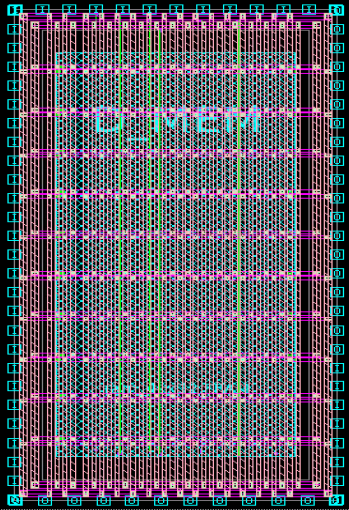
\includegraphics[scale=0.55]{DMEM_cell.png}
\centering
\caption{Foto captura del layout resultante de la impementación del \textit{IP Core} de una memoria SRAM de 4kx32.}
\label{fig:dram_cell}
\end{figure}

Para demostrar la funcionalidad del \textit{IP Core} generado se realiza una pequeña simulación post implementación física. El resultado se aprecia en las figuras \ref{fig:dram_sim_m} y \ref{fig:dram_sim_t}. Puede apreciarse como el dato se escribe (en la dirección ffe) en el primer de reloj, si se presta atención al marcador M1 (línea vertical de color gris) se aprecia entre paréntesis el lapso que existe entre el flanco de la señal de reloj y el cambio en la señal de salida del dato. Este tiempo es distinto para las dos simulaciones siendo mayor en la figura \ref{fig:dram_sim_t} pues considera los retardos máximos del diseño, mientras que la figura \ref{fig:dram_sim_m} muestra el efecto de los retardos mínimos.

\begin{figure}[h]
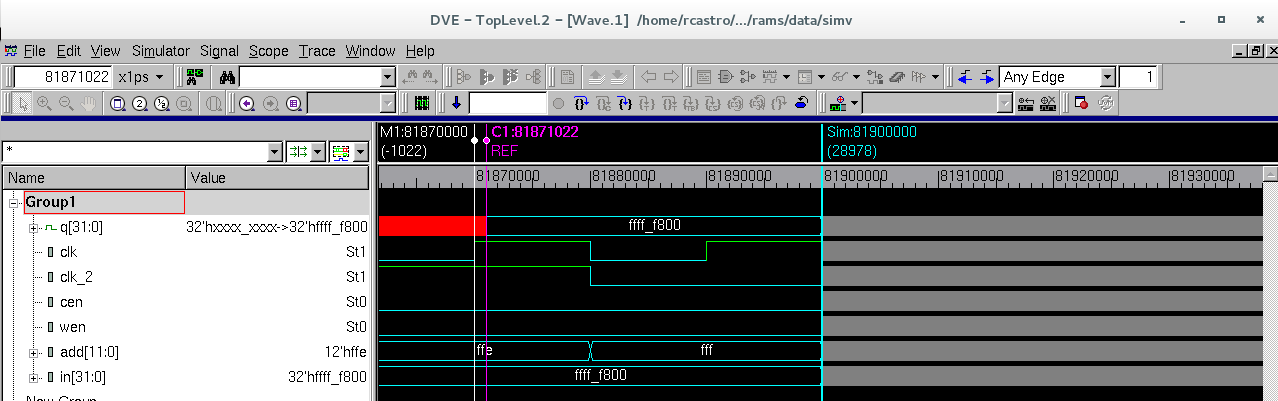
\includegraphics[width=\textwidth]{sim_DMEM_phy_min.png}
\centering
\caption{Simulación post implementación física del \textit{IP Core} para la memoria de datos (4kx32) con el modelo de retardos mínimos}
\label{fig:dram_sim_m}
\end{figure}

\begin{figure}[h]
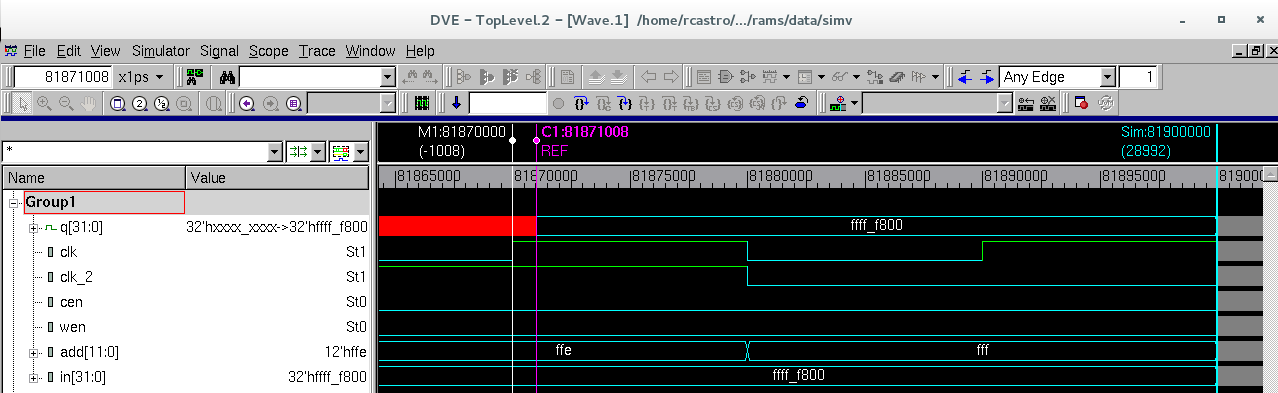
\includegraphics[width=\textwidth]{sim_DMEM_phy_typ.png}
\centering
\caption{Simulación post implementación física del \textit{IP Core} para la memoria de datos (4kx32) con el modelo de retardos típicos}
\label{fig:dram_sim_t}
\end{figure}
  \chapter{Conclusiones y Recomendaciones}

\section{Conclusiones}
Partiendo de una estructura básica para la integración de diseños codificados en RTL se ha logrado diseñar una jerarquía de archivos y directorios que permite implementar exitosamente un flujo de diseño de circuitos integrados digitales.

Mediante el uso de esta jerárquía fue posible implementar una unidad aritmética de punto flotante y demostrar que es correcta y funcional. Así mismo se demostró que es posible incorporar \textit{IP Cores} dentro del diseño y que los mismos son correctos y funcionales.

Debido a particularidades que se escapan de la visión de este trabajo no fue posible demostrar la funcionalidad del microprocesador RISC-V. Debido a deficiencias en la estructura de su RTL, sin embargo, quedó demostrado que el flujo es eficaz y eficiente.

Realizar una evaluación cuantitativa sobre la estructura de \textit{scripting} diseñada no es posible ya que responde a la visión de una única persona, y su paradigma particular de trabajo. Sin embargo, desde una perspectiva cualitativa y subjetiva, se considera la estructura de \textit{scripting} eficiente, pues manifiesta atributos como: regularidad, localidad y continuidad.

\section{Recomendaciones}

Se recomienda realizar una iteración en el diseño del microprocesador ASP, enfocado a incorporar una unidad para la programación de las memorias y permitir el \textit{booteo} del microprocesador.

Finalmente recomienda incorporar en una iteración futura optimizaciones asociadas con el área y la potencia de los módulos, incorporando técnicas como \textit{clock gating}, las cuales no fueron utilizadas en este proyecto.

  %----------------------------------------------------------------------------
  % literature
  \bibliographystyle{sty/plainurl} % for english documents
  \bibliography{literatura}
  %----------------------------------------------------------------------------

  %----------------------------------------------------------------------------
  \appendix
  %----------------------------------------------------------------------------

  \chapter{Hoja de Información del Proyecto}

% El título anterior es solo un ejemplo ilustrativo.  Éste teorema no ameritaría
% un apéndice pues es parte normal del currículum de Electrónica, pero apéndices
% usualmente involucran aspectos de esta índole, que se salen de la línea de la
% tesis, pero que es conveniente incluir por completitud.

% Los anexos contienen toda información adicional que se considere pertinente
% agregar, como manuales de usuario, demostraciones matemáticas que se salen de
% la línea principal de la tesis, pero que pueden considerarse parte de los
% resultados del trabajo.


  %----------------------------------------------------------------------------
  \backmatter
  %----------------------------------------------------------------------------

  \printindex                % insert index into document. Don't forget to call
                             % "makeindex filename" first.
\end{document}
